\def\true{true}
\let\fpacm\true
\documentclass[onecolumn,11pt,nocopyrightspace,preprint]{sigplanconf}
\usepackage{amstext}
\usepackage[T1]{fontenc}
\usepackage[utf8]{inputenc}
\usepackage{moreverb}
\usepackage{tikz}
\usepackage{xspace}
\usepackage{mymacros}
\def\fppdf{true}
\usepackage{fppdf}
% EBNF syntax.

\let\nt\textit % Nonterminal.
\newcommand{\is}{& ${} ::= {}$ &}
\newcommand{\newprod}{\\\hspace{1cm}\barre\hspace{2mm}}
\newcommand{\phaprod}{\\\hspace{1cm}\phantom\barre\hspace{2mm}}
% Options and choices.
\newcommand{\optional}[1]{%
  \ifmmode [\,#1\,]%
  \else    $[\,\text{#1}\,]$%
  \fi
}
\newcommand{\metachoice}{$\,\mid\,$}
% Lists.
\newcommand{\seplist}[2]{#2#1${}\ldots{}$#1#2}
\newcommand{\sepspacelist}[1]{\seplist{\ }{#1}}
\newcommand{\sepcommalist}[1]{\seplist{,\ }{#1}}
\newcommand{\precseplist}[2]{%
  \optional{#1} \seplist{\ #1}{#2}%
}
% Optional parameters.
\newcommand{\tuple}[1]{\dlpar\sepcommalist{#1}\drpar}
\newcommand{\oparams}[1]{\optional{\tuple{#1}}}
% Some nonterminal symbols used in the grammar.
\newcommand{\expression}{\nt{expression}\xspace}
\newcommand{\expressionsub}[1]{\nt{expression}${}_{#1}$}
\newcommand{\pattern}{\nt{pattern}\xspace}

% Concrete syntax.

\newcommand{\percentpercent}{\kw{\%\%}\xspace}
\newcommand{\deuxpoints}{\kw{:}\xspace}
\newcommand{\barre}{\kw{\textbar}\xspace}
\newcommand{\kangle}[1]{\kw{\textless} #1 \kw{\textgreater}}
\newcommand{\ocamltype}{\kangle{\textit{\ocaml type}}\xspace}
\newcommand{\ocamlparam}{\kangle{\nt{uid} \deuxpoints \textit{\ocaml module type}}\xspace}
\newcommand{\dheader}[1]{\kw{\%\{} #1 \kw{\%\}}}
\newcommand{\dtoken}{\kw{\%token}\xspace}
\newcommand{\dstart}{\kw{\%start}\xspace}
\newcommand{\dtype}{\kw{\%type}\xspace}
\newcommand{\dnonassoc}{\kw{\%nonassoc}\xspace}
\newcommand{\dleft}{\kw{\%left}\xspace}
\newcommand{\dright}{\kw{\%right}\xspace}
\newcommand{\dparameter}{\kw{\%parameter}\xspace}
\newcommand{\dpublic}{\kw{\%public}\xspace}
\newcommand{\dinline}{\kw{\%inline}\xspace}
\newcommand{\donerrorreduce}{\kw{\%on\_error\_reduce}\xspace}
\newcommand{\dattribute}{\kw{\%attribute}\xspace}
\newcommand{\dpaction}[1]{\kw{\{} #1 \kw{\}}\xspace}
\newcommand{\daction}{\dpaction{\textit{\ocaml code}}\xspace}
\newcommand{\dpfaction}[1]{\kw{<} #1 \kw{>}\xspace}
\newcommand{\dpfidentityaction}{\kw{<>}\xspace}
\newcommand{\dprec}{\kw{\%prec}\xspace}
\newcommand{\dequal}{\kw{\small =}\xspace}
\newcommand{\dquestion}{\kw{?}\xspace}
\newcommand{\dplus}{\raisebox{2pt}{\kw{\small +}}\xspace}
\newcommand{\dcolonequal}{\kw{\small :=}\xspace}
\newcommand{\dequalequal}{\kw{\small ==}\xspace}
\newcommand{\dstar}{\kw{*}\xspace}
\newcommand{\dlpar}{\kw{(}\,\xspace}
\newcommand{\drpar}{\,\kw{)}\xspace}
\newcommand{\eos}{\kw{\#}\xspace}
\newcommand{\dnewline}{\kw{\textbackslash n}\xspace}
\newcommand{\dlet}{\kw{let}\xspace}
\newcommand{\dsemi}{\kw{;}\xspace}
\newcommand{\dunderscore}{\kw{\_}\xspace}
\newcommand{\dtilde}{\raisebox{-4pt}{\kw{\textasciitilde}}\xspace}

% Stylistic conventions.

\newcommand{\kw}[1]{\text{\upshape\sf\bfseries #1}}
\newcommand{\inlinesidecomment}[1]{\textit{\textbf{\footnotesize // #1}}}
\newcommand{\sidecomment}[1]{\hspace{2cm}\inlinesidecomment{#1}}
\newcommand{\docskip}{\vspace{1mm plus 1mm}}
\newcommand{\docswitch}[1]{\docskip#1.\hspace{3mm}}
\newcommand{\error}{\kw{error}\xspace}

% Links to Menhir's repository.

\newcommand{\repo}[2]{\href{https://gitlab.inria.fr/fpottier/menhir/blob/master/#1}{#2}}
\newcommand{\menhirlibconvert}{\repo{lib/Convert.mli}{\texttt{MenhirLib.Convert}}\xspace}
\newcommand{\menhirliberrorreports}{\repo{lib/ErrorReports.mli}{\texttt{MenhirLib.ErrorReports}}\xspace}
\newcommand{\menhirlibincrementalengine}{\repo{lib/IncrementalEngine.ml}{\texttt{MenhirLib.IncrementalEngine}}\xspace}
\newcommand{\standardmly}{\repo{src/standard.mly}{\texttt{standard.mly}}\xspace}
\newcommand{\distrib}[1]{\repo{#1}{\texttt{#1}}}

% Links to CompCert's repository.

\newcommand{\compcertgithub}{https://github.com/AbsInt/CompCert/tree/master}
\newcommand{\compcertgithubfile}[1]{\href{\compcertgithub/#1}{\texttt{#1}}}

% Abbreviations.

\newcommand{\menhir}{Menhir\xspace}
\newcommand{\menhirlib}{\texttt{MenhirLib}\xspace}
\newcommand{\menhirsdk}{\texttt{MenhirSdk}\xspace}
\newcommand{\coqmenhirlib}{\texttt{MenhirLib}\xspace} % for now
\newcommand{\menhirinterpreter}{\texttt{MenhirInterpreter}\xspace}
\newcommand{\cmenhir}{\texttt{menhir}\xspace}
\newcommand{\ml}{\texttt{.ml}\xspace}
\newcommand{\mli}{\texttt{.mli}\xspace}
\newcommand{\mly}{\texttt{.mly}\xspace}
\newcommand{\cmly}{\texttt{.cmly}\xspace}
\newcommand{\vy}{\texttt{.vy}\xspace}
\newcommand{\ocaml}{OCaml\xspace}
\newcommand{\ocamlc}{\texttt{ocamlc}\xspace}
\newcommand{\ocamlopt}{\texttt{ocamlopt}\xspace}
\newcommand{\ocamldep}{\texttt{ocamldep}\xspace}
\newcommand{\make}{\texttt{make}\xspace}
\newcommand{\omake}{\texttt{omake}\xspace}
\newcommand{\ocamlbuild}{\texttt{ocamlbuild}\xspace}
\newcommand{\dune}{\texttt{dune}\xspace}
\newcommand{\Makefile}{\texttt{Makefile}\xspace}
\newcommand{\yacc}{\texttt{yacc}\xspace}
\newcommand{\bison}{\texttt{bison}\xspace}
\newcommand{\ocamlyacc}{\texttt{ocamlyacc}\xspace}
\newcommand{\ocamllex}{\texttt{ocamllex}\xspace}
\newcommand{\token}{\texttt{token}\xspace}
\newcommand{\automaton}{\texttt{.automaton}\xspace}
\newcommand{\automatonresolved}{\texttt{.automaton.resolved}\xspace}
\newcommand{\conflicts}{\texttt{.conflicts}\xspace}
\newcommand{\dott}{\texttt{.dot}\xspace}
\newcommand{\legacy}{\texttt{legacy}\xspace}
\newcommand{\simplified}{\texttt{simplified}\xspace}

% Environments.

\newcommand{\question}[1]{\vspace{3mm}$\diamond$ \textbf{#1}}

% Ocamlweb settings.

\newcommand{\basic}[1]{\textit{#1}}
\let\ocwkw\kw
\let\ocwbt\basic
\let\ocwupperid\basic
\let\ocwlowerid\basic
\let\ocwtv\basic
\newcommand{\ocwbar}{\vskip 2mm plus 2mm \hrule \vskip 2mm plus 2mm}
\newcommand{\tcup}{${}\cup{}$}
\newcommand{\tcap}{${}\cap{}$}
\newcommand{\tminus}{${}\setminus{}$}

% Command line options.

\newcommand{\oo}[1]{\texttt{-{}-#1}\xspace}

\newcommand{\obase}{\oo{base}}
\newcommand{\ocanonical}{\oo{canonical}} % undocumented!
\newcommand{\ocomment}{\oo{comment}}
\newcommand{\ocmly}{\oo{cmly}}
\newcommand{\odepend}{\oo{depend}}
\newcommand{\orawdepend}{\oo{raw-depend}}
\newcommand{\odump}{\oo{dump}}
\newcommand{\odumpresolved}{\oo{dump-resolved}}
\newcommand{\oerrorrecovery}{\oo{error-recovery}}
\newcommand{\oexplain}{\oo{explain}}
\newcommand{\oexternaltokens}{\oo{external-tokens}}
\newcommand{\ofixedexc}{\oo{fixed-exception}}
\newcommand{\ograph}{\oo{graph}}
\newcommand{\oignoreone}{\oo{unused-token}}
\newcommand{\oignoreall}{\oo{unused-tokens}}
\newcommand{\oignoreprec}{\oo{unused-precedence-levels}}
\newcommand{\oinfer}{\oo{infer}}
\newcommand{\oinferwrite}{\oo{infer-write-query}}
\newcommand{\oinferread}{\oo{infer-read-reply}}
\newcommand{\oinferprotocolsupported}{\oo{infer-protocol-supported}}
\newcommand{\oinspection}{\oo{inspection}}
\newcommand{\ointerpret}{\oo{interpret}}
\newcommand{\ointerpretshowcst}{\oo{interpret-show-cst}}
\newcommand{\ologautomaton}{\oo{log-automaton}}
\newcommand{\ologcode}{\oo{log-code}}
\newcommand{\ologgrammar}{\oo{log-grammar}}
\newcommand{\onodollars}{\oo{no-dollars}}
\newcommand{\onoinline}{\oo{no-inline}}
\newcommand{\onostdlib}{\oo{no-stdlib}}
\newcommand{\oocamlc}{\oo{ocamlc}}
\newcommand{\oocamldep}{\oo{ocamldep}}
\newcommand{\oonlypreprocess}{\oo{only-preprocess}}
\newcommand{\oonlytokens}{\oo{only-tokens}}
\newcommand{\orequirealiases}{\oo{require-aliases}}
\newcommand{\ostrict}{\oo{strict}}
\newcommand{\osuggestcomp}{\oo{suggest-comp-flags}}
\newcommand{\osuggestlinkb}{\oo{suggest-link-flags-byte}}
\newcommand{\osuggestlinko}{\oo{suggest-link-flags-opt}}
\newcommand{\osuggestmenhirlib}{\oo{suggest-menhirLib}}
\newcommand{\osuggestocamlfind}{\oo{suggest-ocamlfind}}
\newcommand{\otable}{\oo{table}}
\newcommand{\otimings}{\oo{timings}}
\newcommand{\otimingsto}{\oo{timings-to}}
\newcommand{\otrace}{\oo{trace}}
\newcommand{\ostdlib}{\oo{stdlib}}
\newcommand{\oversion}{\oo{version}}
\newcommand{\ocoq}{\oo{coq}}
\newcommand{\ocoqlibpath}{\oo{coq-lib-path}}
\newcommand{\ocoqlibnopath}{\oo{coq-lib-no-path}}
\newcommand{\ocoqnocomplete}{\oo{coq-no-complete}}
\newcommand{\ocoqnoactions}{\oo{coq-no-actions}}
\newcommand{\ocoqnoversioncheck}{\oo{coq-no-version-check}}
\newcommand{\olisterrors}{\oo{list-errors}}
\newcommand{\ointerpreterror}{\oo{interpret-error}}
\newcommand{\ocompileerrors}{\oo{compile-errors}}
\newcommand{\ocompareerrors}{\oo{compare-errors}}
\newcommand{\oupdateerrors}{\oo{update-errors}}
\newcommand{\oechoerrors}{\oo{echo-errors}}
\newcommand{\oechoerrorsconcrete}{\oo{echo-errors-concrete}}
\newcommand{\omergeerrors}{\oo{merge-errors}}
\newcommand{\ostrategy}{\oo{strategy}}

% The .messages file format.
\newcommand{\messages}{\text{\tt .messages}\xspace}

% Adding mathstruts to ensure a common baseline.
\newcommand{\mycommonbaseline}{
\let\oldnt\nt
\renewcommand{\nt}[1]{$\mathstrut$\oldnt{##1}}
\let\oldbasic\basic
\renewcommand{\basic}[1]{$\mathstrut$\oldbasic{##1}}
}

% Position keywords.
\newcommand{\ksymbolstartpos}{\texttt{\$symbolstartpos}\xspace}

\gdef\menhirversion{20201216}

% Let Menhir's version number appear at the bottom right of every page.
\makeatletter
\def\@formatyear{\menhirversion}
\makeatother

% Hevea-specific logic; see
%   http://hevea.inria.fr/doc/manual007.html
%   http://hevea.inria.fr/doc/manual008.html
\usepackage{hevea}
\newenvironment{heveapicture}{
\begin{toimage}
}{
\end{toimage}
\imageflush{}
}

% ------------------------------------------------------------------------------

% Headings.

\title{\menhir Reference Manual\\\normalsize (version \menhirversion)}

\begin{document}

\authorinfo{François Pottier\and Yann Régis-Gianas}
	   {INRIA}
	   {\{Francois.Pottier, Yann.Regis-Gianas\}@inria.fr}

\maketitle

% ------------------------------------------------------------------------------

\clearpage
\tableofcontents
\clearpage

% ------------------------------------------------------------------------------

\section{Foreword}

\menhir is a parser generator. It turns high-level grammar specifications,
decorated with semantic actions expressed in the \ocaml programming
language~\cite{ocaml}, into parsers, again expressed in \ocaml. It is
based on Knuth's LR(1) parser construction technique~\cite{knuth-lr-65}. It is
strongly inspired by its precursors: \yacc~\cite{johnson-yacc-79},
\texttt{ML-Yacc}~\cite{tarditi-appel-00}, and \ocamlyacc~\cite{ocaml},
but offers a large number of minor and major improvements that make it a more
modern tool.

This brief reference manual explains how to use \menhir. It does not attempt to
explain context-free grammars, parsing, or the LR technique. Readers who have
never used a parser generator are encouraged to read about these ideas
first~\cite{aho-86,appel-tiger-98,hopcroft-motwani-ullman-00}. They are also
invited to have a look at the \distrib{demos} directory in \menhir's
distribution.

Potential users of \menhir should be warned that \menhir's feature set is not
completely stable. There is a tension between preserving a measure of
compatibility with \ocamlyacc, on the one hand, and introducing new ideas, on
the other hand. Some aspects of the tool, such as the error handling
mechanism, are still potentially subject to incompatible changes: for
instance, in the future, the current error handling mechanism (which is based
on the \error token, see \sref{sec:errors}) could be removed and replaced with
an entirely different mechanism.

There is room for improvement in the tool and in this reference manual. Bug
reports and suggestions are welcome!

% ------------------------------------------------------------------------------

\section{Usage}

\menhir is invoked as follows:
\begin{quote}
\cmenhir \nt{option} \ldots \nt{option} \nt{filename} \ldots \nt{filename}
\end{quote}
Each of the file names must end with \mly (unless \ocoq is used,
in which case it must end with \vy) and denotes a partial
grammar specification. These partial grammar specifications are joined
(\sref{sec:split}) to form a single, self-contained grammar specification,
which is then processed. The following optional command line switches allow
controlling many aspects of the process.

\docswitch{\obase \nt{basename}} This switch controls the base name
of the \ml and \mli files that are produced. That is, the tool will produce
files named \nt{basename}\texttt{.ml} and \nt{basename}\texttt{.mli}. Note
that \nt{basename} can contain occurrences of the \texttt{/} character, so it
really specifies a path and a base name. When only one \nt{filename} is
provided on the command line, the default \nt{basename} is obtained by
depriving \nt{filename} of its final \mly suffix. When multiple file
names are provided on the command line, no default base name exists, so that
the \obase switch \emph{must} be used.

\docswitch{\ocmly} This switch causes \menhir to produce a \cmly file in
addition to its normal operation. This file contains a (binary-form)
representation of the grammar and automaton (see \sref{sec:sdk}).

\docswitch{\ocomment} This switch causes a few comments to be inserted into the
\ocaml code that is written to the \ml file.

\docswitch{\ocompareerrors \nt{filename1} \ocompareerrors \nt{filename2}} Two
such switches must always be used in conjunction so as to specify the names of
two \messages files, \nt{filename1} and \nt{filename2}. Each file is read and
internally translated to a mapping of states to messages. \menhir then checks
that the left-hand mapping is a subset of the right-hand mapping. This feature
is typically used in conjunction with \olisterrors to check that \nt{filename2}
is complete (that is, covers all states where an error can occur).
For more information, see \sref{sec:errors:new}.

\docswitch{\ocompileerrors \nt{filename}} This switch causes \menhir to read the
file \nt{filename}, which must obey the \messages file format, and to compile
it to an \ocaml function that maps a state number to a message. The \ocaml code
is sent to the standard output channel. At the same time, \menhir checks that
the collection of input sentences in the file \nt{filename} is correct and
irredundant. For more information, see \sref{sec:errors:new}.

\docswitch{\ocoq} This switch causes \menhir to produce Coq code. See \sref{sec:coq}.

\docswitch{\ocoqlibpath \nt{path}} This switch allows specifying under what
name (or path) the Coq support library is known to Coq. When \menhir runs in
\ocoq mode, the generated parser contains references to several modules in
this library. This path is used to qualify these references. Its default value
is \coqmenhirlib.

\docswitch{\ocoqlibnopath} This switch indicates that references to the Coq
library \coqmenhirlib should \emph{not} be qualified. This was the default
behavior of \menhir prior to 2018/05/30. This switch is provided for
compatibility, but normally should not be used.

\docswitch{\ocoqnoactions} (Used in conjunction with \ocoq.) This switch
causes the semantic actions present in the \vy file to be ignored and
replaced with \verb+tt+, the unique inhabitant of Coq's \verb+unit+ type. This
feature can be used to test the Coq back-end with a standard grammar, that is, a
grammar that contains \ocaml semantic actions. Just rename the file from
\mly to \vy and set this switch.

\docswitch{\ocoqnocomplete} (Used in conjunction with \ocoq.) This switch
disables the generation of the proof of completeness of the parser
(\sref{sec:coq}). This can be necessary because the proof of completeness is
possible only if the grammar has no conflict (not even a benign one, in the
sense of \sref{sec:conflicts:benign}). This can be desirable also because, for
a complex grammar, completeness may require a heavy certificate and its
validation by Coq may take time.

\docswitch{\ocoqnoversioncheck} (Used in conjunction with \ocoq.) This switch
prevents the generation of the check that verifies that the versions of
\menhir and \coqmenhirlib match.

\docswitch{\odepend} See \sref{sec:build}.

\docswitch{\odump} This switch causes a description of the automaton to be
written to the file \nt{basename}\automaton. This description is written after
benign conflicts have been resolved, before severe conflicts are resolved
(\sref{sec:conflicts}), and before extra reductions are introduced
(\sref{sec:onerrorreduce}).

\docswitch{\odumpresolved} This command line switch causes a description of
the automaton to be written to the file \nt{basename}\automatonresolved. This
description is written after all conflicts have been resolved
(\sref{sec:conflicts}) and after extra reductions have been introduced
(\sref{sec:onerrorreduce}).

\docswitch{\oechoerrors \nt{filename}} This switch causes \menhir to
read the \messages file \nt{filename} and to produce on the standard output
channel just the input sentences. (That is, all messages, blank lines, and
comments are filtered out.) For more information, see \sref{sec:errors:new}.

\docswitch{\oechoerrorsconcrete \nt{filename}} This switch causes \menhir to
read the \messages file \nt{filename} and to produce on the standard output
channel just the input sentences. Each sentence is followed with a comment of
the form \verb+## Concrete syntax: ...+ that shows this sentence in concrete
syntax. This comment is printed only if the user has defined an alias for
every token (\sref{sec:tokens}).

\docswitch{\oexplain} This switch causes conflict explanations to be
written  to the file \nt{basename}\conflicts. See also \sref{sec:conflicts}.

\docswitch{\oexternaltokens \nt{T}} This switch causes the definition of
the \token type to be omitted in \nt{basename}\texttt{.ml} and
\nt{basename}\texttt{.mli}. Instead, the generated parser relies on
the type $T$\texttt{.}\token, where $T$ is an \ocaml module name. It is up to
the user to define module $T$ and to make sure that it exports a suitable
\token type. Module $T$ can be hand-written. It can also be automatically generated
out of a grammar specification using the \oonlytokens switch.

\docswitch{\ofixedexc} This switch causes the exception \texttt{Error} to be
internally defined as a synonym for \texttt{Parsing.Parse\_error}. This means
that an exception handler that catches \texttt{Parsing.Parse\_error} will also
catch the generated parser's \texttt{Error}. This helps increase \menhir's
compatibility with \ocamlyacc. There is otherwise no reason to use this switch.

\docswitch{\ograph} This switch causes a description of the grammar's
dependency graph to be written to the file \nt{basename}\dott. The graph's
vertices are the grammar's nonterminal symbols. There is a directed edge from
vertex $A$ to vertex $B$ if the definition of $A$ refers to $B$. The file is
in a format that is suitable for processing by the \emph{graphviz} toolkit.

\docswitch{\oinfer, \oinferwrite, \oinferread} See \sref{sec:build}.

\docswitch{\oinspection} This switch requires \otable. It causes \menhir to generate
not only the monolithic and incremental APIs (\sref{sec:monolithic},
\sref{sec:incremental}), but also the inspection API (\sref{sec:inspection}).
Activating this switch causes a few more tables to be produced, resulting in
somewhat larger code size.

\docswitch{\ointerpret} This switch causes \menhir to act as an interpreter,
rather than as a compiler. No \ocaml code is generated. Instead, \menhir
reads sentences off the standard input channel, parses them, and displays
outcomes. This switch can be usefully combined with \otrace.
For more information, see \sref{sec:interpret}.

\docswitch{\ointerpreterror} This switch is analogous to \ointerpret, except
\menhir expects every sentence to cause an error on its last token, and
displays information about the state in which the error is detected, in
the \messages file format. For more information, see \sref{sec:errors:new}.

\docswitch{\ointerpretshowcst} This switch, used in conjunction with \ointerpret,
causes \menhir to display a concrete syntax tree when a sentence is successfully
parsed. For more information, see \sref{sec:interpret}.

\docswitch{\olisterrors} This switch causes \menhir to produce (on the standard
output channel) a complete list of input sentences that cause an error, in the
\messages file format. For more information, see \sref{sec:errors:new}.

\docswitch{\ologautomaton \nt{level}} When \nt{level} is nonzero, this switch
causes some information about the automaton to be logged to the standard error
channel.

\docswitch{\ologcode \nt{level}} When \nt{level} is nonzero, this switch
causes some information about the generated \ocaml code to be logged to the
standard error channel.

\docswitch{\ologgrammar \nt{level}} When \nt{level} is nonzero, this switch
causes some information about the grammar to be logged to the standard error
channel. When \nt{level} is 2, the \emph{nullable}, \emph{FIRST}, and
\emph{FOLLOW} tables are displayed.

\docswitch{\omergeerrors \nt{filename1} \omergeerrors \nt{filename2}} Two such
switches must always be used in conjunction so as to specify the names of two
\messages files, \nt{filename1} and \nt{filename2}. This command causes
\menhir to merge these two \messages files and print the result on the
standard output channel. For more information, see \sref{sec:errors:new}.

\docswitch{\onodollars} This switch disallows the use of positional keywords
of the form \kw{\$i}.

\docswitch{\onoinline} This switch causes all \dinline keywords in the
grammar specification to be ignored. This is especially useful in order
to understand whether these keywords help solve any conflicts.

\docswitch{\onostdlib} This switch instructs \menhir to \emph{not} use
its standard library (\sref{sec:library}).

\docswitch{\oocamlc \nt{command}} See \sref{sec:build}.

\docswitch{\oocamldep \nt{command}} See \sref{sec:build}.

\docswitch{\oonlypreprocess} This switch causes the grammar specifications
to be transformed up to the point where the automaton's construction can
begin. The grammar specifications whose names are provided on the command line
are joined (\sref{sec:split}); all parameterized nonterminal symbols are
expanded away (\sref{sec:templates}); type inference is performed, if \oinfer
is enabled; all nonterminal symbols marked \dinline are expanded away
(\sref{sec:inline}). This yields a single, monolithic grammar specification,
which is printed on the standard output channel.

\docswitch{\oonlytokens} This switch causes the \dtoken declarations in
the grammar specification to be translated into a definition of the \token
type, which is written to the files \nt{basename}\texttt{.ml} and
\nt{basename}\texttt{.mli}. No code is generated. This is useful when
a single set of tokens is to be shared between several parsers. The directory
\distrib{demos/calc-two} contains a demo that illustrates the use of this switch.

\docswitch{\orawdepend} See \sref{sec:build}.

\docswitch{\orequirealiases} This switch causes \menhir to check that a token
alias (\sref{sec:tokens}) has been defined for every token. There is no
requirement for this alias to be actually used; it must simply exist. A
missing alias gives rise to a warning (and, in \ostrict mode, to an error).

\docswitch{\ostdlib \nt{directory}} This switch exists only for
backwards compatibility and is ignored. It may be removed in the future.

\docswitch{\ostrategy \nt{strategy}} This switch selects an error handling
strategy, to be used by the code back-end, the table back-end, and the
reference interpreter. The available strategies are \legacy and
simplified. (However, at the time of writing, the code back-end does
not yet support the simplified strategy.) When this switch is
omitted, the \legacy strategy is used. The choice of a strategy
matters only if the grammar uses the \error token. For more details, see
\sref{sec:errors}.

\docswitch{\ostrict} This switch causes several warnings about the grammar
and about the automaton to be considered errors. This includes warnings about
useless precedence declarations, non-terminal symbols that produce the empty
language, unreachable non-terminal symbols, productions that are never
reduced, conflicts that are not resolved by precedence declarations,
end-of-stream conflicts, and missing token aliases.

\docswitch{\oo{suggest-*}} See \sref{sec:build}.

\docswitch{\otable} This switch causes \menhir to use its table-based
back-end, as opposed to its (default) code-based back-end. When \otable is
used, \menhir produces significantly more compact and somewhat slower parsers.
See \sref{sec:qa} for a speed comparison.

The table-based back-end produces rather compact tables, which are analogous
to those produced by \yacc, \bison, or \ocamlyacc. These tables are not quite
stand-alone: they are exploited by an interpreter, which is shipped as part of
the support library \menhirlib. For this reason, when \otable is used,
\menhirlib must be made visible to the \ocaml compilers, and must be linked
into your executable program. The \texttt{--suggest-*} switches, described
above, help do this.

The code-based back-end compiles the LR automaton directly into a nest of
mutually recursive \ocaml functions. In that case, \menhirlib is not required.

The incremental API (\sref{sec:incremental}) and the inspection API
(\sref{sec:inspection}) are made available only by the table-based back-end.

\docswitch{\otimings} This switch causes internal timing information to
be sent to the standard error channel.

\docswitch{\otimingsto \nt{filename}} This switch causes internal timing
information to be written to the file \nt{filename}.

\docswitch{\otrace} This switch causes tracing code to be inserted into
the generated parser, so that, when the parser is run, its actions are
logged to the standard error channel. This is analogous to \texttt{ocamlrun}'s
\texttt{p=1} parameter, except this switch must be enabled at compile time:
one cannot selectively enable or disable tracing at runtime.

\docswitch{\oignoreprec} This switch suppresses all warnings about
useless \dleft, \dright, \dnonassoc and \dprec declarations.

\docswitch{\oignoreone \nt{symbol}} This switch suppresses the warning that
is normally emitted when \menhir finds that the terminal symbol \nt{symbol} is
unused.

\docswitch{\oignoreall} This switch suppresses all of the warnings that are
normally emitted when \menhir finds that some terminal symbols are unused.

\docswitch{\oupdateerrors \nt{filename}} This switch causes \menhir to
read the \messages file \nt{filename} and to produce on the standard output
channel a new \messages file that is identical, except the auto-generated
comments have been re-generated. For more information,
see \sref{sec:errors:new}.

\docswitch{\oversion} This switch causes \menhir to print its own version
number and exit.

% ------------------------------------------------------------------------------

\section{Lexical conventions}

A semicolon character (\kw{;}) \emph{may} appear after a declaration
(\sref{sec:decls}).

An old-style rule (\sref{sec:old:rules}) \emph{may} be terminated with a
semicolon. Also, within an old-style rule, each producer
(\sref{sec:producers}) \emph{may} be terminated with a semicolon.

A new-style rule (\sref{sec:new:rules}) \emph{must not} be terminated with a
semicolon. Within such a rule, the elements of a sequence \emph{must} be
separated with semicolons.

Semicolons are not allowed to appear anywhere except in the places mentioned
above. This is in contrast with \ocamlyacc, which views semicolons as
insignificant, just like whitespace.

Identifiers (\nt{id}) coincide with \ocaml identifiers, except they are not
allowed to contain the quote (\kw{'}) character. Following
\ocaml, identifiers that begin with a lowercase letter
(\nt{lid}) or with an uppercase letter (\nt{uid}) are distinguished.

A quoted identifier \nt{qid} is a string enclosed in double quotes.
Such a string cannot contain a double quote or a backslash.
Quoted identifiers are used as token aliases (\sref{sec:tokens}).

Comments are C-style (surrounded with \kw{/*} and \kw{*/}, cannot be nested),
C++-style (announced by \kw{/$\!$/} and extending until the end of the line), or
\ocaml-style (surrounded with \kw{(*} and \kw{*)}, can be nested). Of course,
inside \ocaml code, only \ocaml-style comments are allowed.

\ocaml type expressions are surrounded with \kangle{and}. Within such expressions,
all references to type constructors (other than the built-in \textit{list}, \textit{option}, etc.)
must be fully qualified.

% ------------------------------------------------------------------------------

\section{Syntax of grammar specifications}

\newcommand{\modifier}{(\,\dquestion \metachoice \dplus \metachoice \dstar\hspace{-.3mm})}

\begin{figure}
\begin{center}
\begin{tabular}{r@{}c@{}l}

\nt{specification} \is
   \sepspacelist{\nt{declaration}}
   \percentpercent
   \sepspacelist{\nt{rule}}
   \optional{\percentpercent \textit{\ocaml code}} \\

\nt{declaration} \is
   \dheader{\textit{\ocaml code}} \\
&& \dparameter \ocamlparam \\
&& \dtoken \optional{\ocamltype} \sepspacelist{\nt{uid} \optional{\nt{qid}}} \\
&& \dnonassoc \sepspacelist{\nt{uid}} \\
&& \dleft \sepspacelist{\nt{uid}} \\
&& \dright \sepspacelist{\nt{uid}} \\
&& \dtype \ocamltype \sepspacelist{\nt{lid}} \\
&& \dstart \optional{\ocamltype} \sepspacelist{\nt{lid}} \\
&& \dattribute \sepspacelist{\nt{actual}} \sepspacelist{\nt{attribute}} \\
&& \kw{\%} \nt{attribute} \\ % a grammar-wide attribute
&& \donerrorreduce \sepspacelist{\nt{lid}} \\
\nt{attribute} \is
    \kw{[@} \nt{name} \nt{payload} \kw{]}
\\[4mm]

\emph{old syntax} ---
\nt{rule} \is
   \optional{\dpublic} \optional{\dinline}
   \nt{lid}
   \oparams{\nt{id}}
   \deuxpoints
   \precseplist\barre{\nt{group}} \\

\nt{group} \is
   \seplist{\ \barre}{\nt{production}}
   \daction
   \optional {\dprec \nt{id}} \\

\nt{production} \is
   \sepspacelist{\nt{producer}} \optional {\dprec \nt{id}} \\

\nt{producer} \is
   \optional{\nt{lid} \dequal} \nt{actual} \\

\nt{actual} \is
   \nt{id} \oparams{\nt{actual}} \\
&& \nt{actual} \modifier \\
&& \seplist{\ \barre}{\nt{group}} % not really allowed everywhere
\\[4mm]

\emph{new syntax} ---
\nt{rule} \is
  \optional{\dpublic}
  \dlet
  \nt{lid}
  \oparams{\nt{id}}
  (\,\dcolonequal \metachoice \dequalequal\hspace{-.2mm})
  \expression
\\
\expression \is
  % a choice between sequence expressions:
  \precseplist\barre\expression
\\&&
  % a sequence expression:
  \optional{\pattern \dequal{}} \expression \dsemi \expression
\\&&
  % a symbol expression:
  \nt{id} \oparams{\expression}
\\&&
  % a symbol expression:
  \expression \modifier
\\&&
  % an action expression:
  \daction
  \optional {\dprec \nt{id}}
    % %prec is in fact allowed to appear before the semantic action,
    % but this is not documented.
\\&&
  % an action expression:
  \dpfaction{\nt{\ocaml id}}
  \optional {\dprec \nt{id}}
\\
\pattern \is
  \nt{lid}
\,\metachoice\,
  \dunderscore
\,\metachoice\,
  \dtilde
\,\metachoice\,
  \tuple\pattern

% The places where attributes can be attached are not shown in this
% figure. This is intentional; let's avoid pollution. Attributes are
% described separately.
\end{tabular}
\end{center}
\caption{Syntax of grammar specifications}
\label{fig:syntax}
\end{figure}

The syntax of grammar specifications appears in \fref{fig:syntax}.
The places where attributes can be attached are not shown; they
are documented separately (\sref{sec:attributes}).
%
% (For compatibility with \ocamlyacc, some specifications that do not fully
% adhere to this syntax are also accepted.)
%
A grammar specification begins with a sequence of declarations
(\sref{sec:decls}), ended by a mandatory \percentpercent keyword.
%
Following this keyword, a sequence of rules is expected.
Each rule defines a nonterminal symbol~\nt{lid},
whose name must begin with a lowercase letter.
%
% In reality, in the old syntax, this is enforced only for start symbols.
% In the new syntax, this is enforced for all symbols.
%
% A rule can also *extend* a symbol, but let's not mention that here.
%
A rule is expressed either in the ``old syntax'' (\sref{sec:old:rules}) or in the
``new syntax'' (\sref{sec:new:rules}), which is slightly more elegant and
powerful.

\subsection{Declarations}
\label{sec:decls}

\subsubsection{Headers}
\label{sec:decls:headers}

A header is a piece of \ocaml code, surrounded with \dheader{and}. It is
copied verbatim at the beginning of the \ml file. It typically contains \ocaml
\kw{open} directives and function definitions for use by the semantic
actions. If a single grammar specification file contains multiple headers,
their order is preserved. However, when two headers originate in distinct
grammar specification files, the order in which they are copied to the \ml
file is unspecified.

It is important to note that the header is copied by \menhir only to the \ml
file, \emph{not} to the \mli file. Therefore, it should not contain
declarations that affect the meaning of the types that appear in the \mli
file. Here are two problems that people commonly run into:
\begin{itemize}
\item Placing an \kw{open} directive that is required for a \dtype declaration
  to make sense. For instance, writing \verb+open Foo+ in the header and
  declaring \verb+%type<t> bar+, where the type \verb+t+ is defined in the
  module \verb+Foo+, will not work. You must write \verb+%type<Foo.t> bar+.
\item Declaring a module alias that affects a (declared or inferred) type. For
  instance, writing \verb+module F = Foo+ in the header and declaring
  \verb+%type<Foo.t> bar+ may not work (from
  2020/05/25 on). The reason is, OCaml may infer that the symbol \verb+bar+ has
  type \verb+F.t+, and Menhir will rely on this information without realizing
  that \verb+F+ is a local name, so in the end, the \mli file contains a
  reference to \verb+F.t+ that does not make sense.
\end{itemize}

\subsubsection{Parameters}
\label{sec:parameter}

A declaration of the form:
\begin{quote}
\dparameter \ocamlparam
\end{quote}
causes the entire parser to become parameterized over the \ocaml module
\nt{uid}, that is, to become an \ocaml functor. The directory
\distrib{demos/calc-param} contains a demo that illustrates the use of this switch.

If a single specification file
contains multiple \dparameter declarations, their order is preserved, so that
the module name \nt{uid} introduced by one declaration is effectively in scope
in the declarations that follow. When two \dparameter declarations originate
in distinct grammar specification files, the order in which they are processed
is unspecified. Last, \dparameter declarations take effect before \dheader{$\ldots$},
\dtoken, \dtype, or \dstart declarations are considered, so that the module name
\nt{uid} introduced by a \dparameter declaration is effectively in scope in
\emph{all} \dheader{$\ldots$}, \dtoken, \dtype, or \dstart declarations,
regardless of whether they precede or follow the \dparameter declaration.
This means, in particular, that the side effects of an \ocaml header are
observed only when the functor is applied, not when it is defined.

\subsubsection{Tokens}
\label{sec:tokens}

A declaration of the form:
\begin{quote}
\dtoken
\optional{\ocamltype}
$\nt{uid}_1$ \optional{$\nt{qid}_1$} $\;\ldots\;$
$\nt{uid}_n$ \optional{$\nt{qid}_n$}
\end{quote}
defines the identifiers $\nt{uid}_1, \ldots, \nt{uid}_n$ as tokens, that is,
as terminal symbols in the grammar specification and as data constructors in
the \textit{token} type.

If an \ocaml type $t$ is present, then these tokens are considered to carry a
semantic value of type $t$, otherwise they are considered to carry no semantic
value.

If a quoted identifier $\nt{qid}_i$ is present, then it is considered an alias
for the terminal symbol $\nt{uid}_i$. (This feature, known as ``token
aliases'', is borrowed from Bison.)
% https://www.gnu.org/software/bison/manual/html_node/Token-Decl.html#Token-Decl
Throughout the grammar, the quoted identifier $\nt{qid}_i$ is then
synonymous with the identifier $\nt{uid}_i$.
%
For example, if one declares:
\begin{verbatim}
%token PLUS "+"
\end{verbatim}
then the quoted identifier \texttt{"+"} stands for the terminal symbol
\texttt{PLUS} throughout the grammar. An example of the use of token aliases
appears in the directory \distrib{demos/calc-alias}.
%
Token aliases can be used to improve the readability of a grammar. One must
keep in mind, however, that they are just syntactic sugar: they are not
interpreted in any way by Menhir or conveyed to tools like \ocamllex.
%
They could be considered confusing by a reader who mistakenly believes that
they are interpreted as string literals.

\subsubsection{Priority and associativity}
\label{sec:assoc}

A declaration of one of the following forms:
\begin{quote}
\dnonassoc $\nt{uid}_1 \ldots \nt{uid}_n$ \\
\dleft $\nt{uid}_1 \ldots \nt{uid}_n$ \\
\dright $\nt{uid}_1 \ldots \nt{uid}_n$
\end{quote}
assigns both a \emph{priority level} and an \emph{associativity status} to
the symbols $\nt{uid}_1, \ldots, \nt{uid}_n$. The priority level assigned to
$\nt{uid}_1, \ldots, \nt{uid}_n$ is not defined explicitly: instead, it is
defined to be higher than the priority level assigned by the previous
\dnonassoc, \dleft, or \dright declaration, and lower than that assigned by the next
\dnonassoc, \dleft, or \dright declaration. The symbols $\nt{uid}_1, \ldots, \nt{uid}_n$
can be tokens (defined elsewhere by a \dtoken declaration) or dummies (not
defined anywhere). Both can be referred to as part of \dprec annotations.
Associativity status and priority levels allow shift/reduce conflicts to be
silently resolved (\sref{sec:conflicts}).

\subsubsection{Types}
\label{sec:type}

A declaration of the form:
\begin{quote}
\dtype \ocamltype $\nt{lid}_1 \ldots \nt{lid}_n$
\end{quote}
assigns an \ocaml type to each of the nonterminal symbols $\nt{lid}_1, \ldots, \nt{lid}_n$.
For start symbols, providing an \ocaml type is mandatory, but is usually done as part of the
\dstart declaration. For other symbols, it is optional. Providing type information can improve
the quality of \ocaml's type error messages.

A \dtype declaration may concern not only a nonterminal symbol, such as, say,
\texttt{expression}, but also a fully applied parameterized nonterminal
symbol, such as \texttt{list(expression)} or \texttt{separated\_list(COMMA,
  option(expression))}.

The types provided as part of \dtype declarations are copied verbatim to the
\ml and \mli files. In contrast, headers (\sref{sec:decls:headers}) are copied
to the \ml file only. For this reason, the types provided as part of \dtype
declarations must make sense both in the presence and in the absence of these
headers. They should typically be fully qualified types.

% TEMPORARY type information can be mandatory in --coq mode; document?

\subsubsection{Start symbols}
\label{sec:start}

A declaration of the form:
\begin{quote}
\dstart \optional{\ocamltype} $\nt{lid}_1 \ldots \nt{lid}_n$
\end{quote}
declares the nonterminal symbols $\nt{lid}_1, \ldots, \nt{lid}_n$ to be
start symbols. Each such symbol must be assigned an \ocaml type either as
part of the \dstart declaration or via separate \dtype declarations. Each
of $\nt{lid}_1, \ldots, \nt{lid}_n$ becomes the name of a function whose
signature is published in the \mli file and that can be used to invoke
the parser.

\subsubsection{Attribute declarations}

Attribute declarations
of the form
\dattribute \sepspacelist{\nt{actual}} \sepspacelist{\nt{attribute}}
and
\kw{\%} \nt{attribute}
are explained
in \sref{sec:attributes}.

\subsubsection{Extra reductions on error}
\label{sec:onerrorreduce}

A declaration of the form:
\begin{quote}
\donerrorreduce $\nt{lid}_1 \ldots \nt{lid}_n$
\end{quote}
marks the nonterminal symbols $\nt{lid}_1, \ldots, \nt{lid}_n$ as
potentially eligible for reduction when an invalid token is found.
This may cause one or more extra reduction steps to be performed
before the error is detected.

More precisely, this declaration affects the automaton as follows. Let us say
that a production $\nt{lid} \rightarrow \ldots$ is ``reducible on error'' if
its left-hand symbol~\nt{lid} appears in a \donerrorreduce declaration. After
the automaton has been constructed and after any conflicts have been resolved,
in every state~$s$, the following algorithm is applied:
\begin{enumerate}
\item Construct the set of all productions that are ready to be reduced in
  state~$s$ and are reducible on error;
\item Test if one of them, say $p$, has higher ``on-error-reduce-priority''
  than every other production in this set;
\item If so, in state~$s$, replace every error action with a reduction of the
  production~$p$.
(In other words, for every terminal symbol~$t$, if the action table
says: ``in state~$s$, when the next input symbol is~$t$, fail'', then this
entry is replaced with: ``in state~$s$, when the next input symbol
is~$t$, reduce production~$p$''.)
\end{enumerate}

If step 3 above is executed in state~$s$, then an error can never be detected
in state~$s$, since all error actions in state~$s$ are replaced with reduce
actions. Error detection is deferred: at least one reduction takes place
before the error is detected. It is a ``spurious'' reduction: in a canonical
LR(1) automaton, it would not take place.

An \donerrorreduce declaration does not affect the language that is accepted
by the automaton. It does not affect the location where an error is detected.
It is used to control in which state an error is detected. If used wisely, it
can make errors easier to report, because they are detected in a state for
which it is easier to write an accurate diagnostic message
(\sref{sec:errors:diagnostics}).

% This may make the tables bigger (but I have no statistics).
% This makes LRijkstra significantly slower.

Like a \dtype declaration, an \donerrorreduce declaration may concern not only
a nonterminal symbol, such as, say, \texttt{expression}, but also a fully
applied parameterized nonterminal symbol, such as \texttt{list(expression)} or
\texttt{separated\_list(COMMA, option(expression))}.

The ``on-error-reduce-priority'' of a production is that of its left-hand
symbol. The ``on-error-reduce-priority'' of a nonterminal symbol is determined
implicitly by the order of \donerrorreduce declarations. In the declaration
$\donerrorreduce\;\nt{lid}_1 \ldots \nt{lid}_n$, the symbols $\nt{lid}_1, \ldots,
\nt{lid}_n$ have the same ``on-error-reduce-priority''. They have higher
``on-error-reduce-priority'' than the symbols listed in previous
\donerrorreduce declarations, and lower ``on-error-reduce-priority''
than those listed in later \donerrorreduce declarations.

\subsection{Rules---old syntax}
\label{sec:old:rules}

In its simplest
form, a rule begins with the nonterminal symbol \nt{lid},
followed by a colon character (\deuxpoints),
and continues with a sequence of production groups
(\sref{sec:productiongroups}). Each production group is preceded with a
vertical bar character (\barre); the very first bar is optional. The meaning
of the bar is choice: the nonterminal symbol \nt{id} develops to either of the
production groups. We defer explanations of the keyword \dpublic
(\sref{sec:split}), of the keyword \dinline (\sref{sec:inline}), and of the
optional formal parameters $\tuple{\nt{id}}$
(\sref{sec:templates}).

\subsubsection{Production groups}
\label{sec:productiongroups}

In its simplest form, a production group consists of a single production (\sref{sec:productions}),
followed by an \ocaml semantic action (\sref{sec:actions}) and an optional
\dprec annotation (\sref{sec:prec}). A production specifies a sequence of terminal and
nonterminal symbols that should be recognized, and optionally binds
identifiers to their semantic values.

\paragraph{Semantic actions}
\label{sec:actions}

A semantic action is a piece of \ocaml code that is executed in order to
assign a semantic value to the nonterminal symbol with which this production
group is associated. A semantic action can refer to the (already computed)
semantic values of the terminal or nonterminal symbols that appear in the
production via the semantic value identifiers bound by the production.

For compatibility with \ocamlyacc, semantic actions can also refer to
unnamed semantic values via positional keywords of the form
\kw{\$1}, \kw{\$2}, etc.\ This style is discouraged.
(It is in fact forbidden if \onodollars is turned on.)
Furthermore, as
a positional keyword of the form \kw{\$i} is internally rewritten as
\nt{\_i}, the user should not use identifiers of the form \nt{\_i}.

\paragraph{\dprec annotations}
\label{sec:prec}

An annotation of the form \dprec \nt{id} indicates that the precedence level
of the production group is the level assigned to the symbol \nt{id} via a
previous \dnonassoc, \dleft, or \dright declaration (\sref{sec:assoc}). In the
absence of a
\dprec annotation, the precedence level assigned to each production is the
level assigned to the rightmost terminal symbol that appears in it. It is
undefined if the rightmost terminal symbol has an undefined precedence level
or if the production mentions no terminal symbols at all. The precedence level
assigned to a production is used when resolving shift/reduce conflicts
(\sref{sec:conflicts}).

\paragraph{Multiple productions in a group}

If multiple productions are present in a single group, then the semantic
action and precedence annotation are shared between them. This short-hand
effectively allows several productions to share a semantic action and
precedence annotation without requiring textual duplication. It is legal only
when every production binds exactly the same set of semantic value identifiers
and when no positional semantic value keywords (\kw{\$1}, etc.) are used.

\subsubsection{Productions}
\label{sec:productions}

A production is a sequence of producers (\sref{sec:producers}), optionally
followed by a \dprec annotation (\sref{sec:prec}). If a precedence annotation
is present, it applies to this production alone, not to other productions in
the production group. It is illegal for a production and its production group
to both carry \dprec annotations.

\subsubsection{Producers}
\label{sec:producers}

A producer is an actual (\sref{sec:actual}), optionally preceded with a
binding of a semantic value identifier, of the form \nt{lid} \dequal. The
actual specifies which construction should be recognized and how a semantic
value should be computed for that construction. The identifier \nt{lid}, if
present, becomes bound to that semantic value in the semantic action that
follows. Otherwise, the semantic value can be referred to via a positional
keyword (\kw{\$1}, etc.).

\subsubsection{Actuals}
\label{sec:actual}

In its simplest form, an actual is just a terminal or nonterminal symbol
$\nt{id}$. If it is a parameterized non-terminal symbol (see
\sref{sec:templates}), then it should be applied:
$\nt{id}\tuple{\nt{actual}}$.

An actual may be followed with a modifier (\dquestion, \dplus, or
\dstar). This is explained further on (see \sref{sec:templates} and
\fref{fig:sugar}).

An actual may also be an ``anonymous rule''. In that case, one writes
just the rule's right-hand side, which takes the form $\seplist{\ \barre\
}{\nt{group}}$.
(This form is allowed only as an argument in an application.)
This form is expanded on the fly to a definition of a fresh non-terminal
symbol, which is declared \dinline.
For instance, providing an anonymous rule as an argument to \nt{list}:
\begin{quote}
\begin{tabular}{l}
\nt{list} \dlpar \basic{e} = \nt{expression}; \basic{SEMICOLON} \dpaction{\basic{e}} \drpar
\end{tabular}
\end{quote}
is equivalent to writing this:
\begin{quote}
\begin{tabular}{l}
\nt{list} \dlpar \nt{expression\_SEMICOLON} \drpar
\end{tabular}
\end{quote}
where the non-terminal symbol \nt{expression\_SEMICOLON} is chosen fresh and is defined as follows:
\begin{quote}
\begin{tabular}{l}
\dinline \nt{expression\_SEMICOLON}:
\newprod \basic{e} = \nt{expression}; \basic{SEMICOLON} \dpaction{\basic{e}}
\end{tabular}
\end{quote}

\subsection{Rules---new syntax}
\label{sec:new:rules}

Please be warned that \textbf{the new syntax is considered experimental}
and is subject to change in the future.
% TEMPORARY à supprimer un jour...

In its simplest form,
a rule takes the form
\dlet \nt{lid} \dcolonequal \expression.
%
Its left-hand side \nt{lid} is a nonterminal symbol;
its right-hand side is an expression.
%
Such a rule defines an ordinary nonterminal symbol,
while the alternate form
\dlet \nt{lid} \dequalequal \expression
defines an \dinline nonterminal symbol (\sref{sec:inline}),
that is, a macro.
%
A rule can be preceded with the keyword \dpublic (\sref{sec:split})
and can be parameterized with a tuple of formal parameters
$\tuple{\nt{id}}$ (\sref{sec:templates}).
%
The various forms of expressions, listed in \fref{fig:syntax}, are:
%
\begin{itemize}
\item
  A \textbf{choice} between several expressions,
  % \precseplist\barre\expression.
  \optional{\barre}
  \expressionsub{1} \barre ${}\ldots{}$ \barre\expressionsub{n}.
  The leading bar is optional.

\item
  A \textbf{sequence} of two expressions,
  \pattern \dequal \expressionsub{1} \dsemi \expressionsub{2}.
  The semantic value produced by \expressionsub{1}
  is decomposed according to the pattern \pattern.
  The \ocaml variables introduced by \pattern
  may appear in a semantic action
  that ends the sequence \expressionsub{2}.

\item
  A sequence \dtilde \dequal \nt{id}${}_1$ \dsemi \expressionsub{2},
  which is sugar for \nt{id}${}_1$ \dequal \nt{id}${}_1$ \dsemi
  \expressionsub{2}.
  This is a \textbf{pun}.
  % This is a special case of the previous form,
  % yet it receives special treatment; this is the
  % only case where ~ represents a deterministically-chosen name.

\item
  A sequence \expressionsub{1} \dsemi \expressionsub{2},
  which is sugar for
  \dunderscore \dequal \expressionsub{1} \dsemi \expressionsub{2}.

\item
  A \textbf{symbol} \nt{id}, possibly applied to
  a tuple of expressions
  \dlpar \expressionsub{1},\ ${}\ldots{}$,\ \expressionsub{n} \drpar.
  It is worth noting that such an expression \emph{can} form the
  end of a sequence: \nt{id} at the end of a sequence stands for
  \nt{x} \dequal \nt{id} \dsemi \dpaction{\nt{x}}
  for some fresh variable \nt{x}.
  Thus, a sequence need not end with a semantic action.

\item
  An expression followed with \dquestion, \dplus, or \dstar. This is sugar
  for the previous form: see \sref{sec:templates} and \fref{fig:sugar}.

\item
  A \textbf{semantic action} \daction,
  possibly followed with a precedence annotation \dprec \nt{id}.
  This \ocaml code can refer to the variables that have been bound
  earlier in the sequence that this semantic action ends.
  These include all variables named by the user as well as all
  variables introduced by a $\dtilde$ pattern as part of a pun.
  % (but not variables introduced by deep ~ patterns)
  The notation $\kw{\$}i$, where $i$ is an integer, is forbidden.

\item
  A \textbf{point-free semantic action} \dpfaction{\nt{\ocaml id}},
  possibly followed with a precedence annotation \dprec~\nt{id}.
  The \ocaml identifier \nt{id} must denote a function or a data
  constructor. It is applied to a tuple of the variables that have
  been bound earlier in the sequence that this semantic action ends.
  Thus, $\dpfaction{\,\nt{id}\,}$ is sugar for
  $\dpaction{\,\nt{id}\;\,(x_1, \ldots, x_n)\,}$,
  where $x_1, \ldots, x_n$ are the variables bound earlier.
  These include all variables named by the user as well as all
  variables introduced by a $\dtilde$ pattern.

\item
  An identity semantic action \dpfidentityaction. This is sugar for
  \dpfaction{\nt{identity}}, where \nt{identity} is \ocaml's
  identity function.
  Therefore, it is sugar for
  $\dpaction{\,(x_1, \ldots, x_n)\,}$,
  where $x_1, \ldots, x_n$ are the variables bound earlier.
\end{itemize}

\begin{comment}
% fp: not sure if this paragraph is helpful.
To some degree, an expression is analogous to an \ocaml expression: it returns
an \ocaml value, and as a side effect, recognizes and consumes a fragment of
the input. In particular, a sequence
%
\pattern \dequal \expressionsub{1} \dsemi \expressionsub{2}
%
is roughly analogous to an \ocaml sequence \verb+let p = e1 in e2+.
% terminal symbol = recognize and consume one input symbol
% nonterminal symbol = procedure call or macro invocation (if %inline)
% semantic action = OCaml code insertion
\end{comment}

The syntax of expressions, as presented in \fref{fig:syntax}, seems more
permissive than it really is. In reality, a choice cannot be nested inside a
sequence;
% (either on the left or on the right)
a sequence cannot be nested in the left-hand side of a sequence; a semantic
action cannot appear in the left-hand side of a sequence. (Thus, there is a
stratification in three levels: choice expressions, sequence expressions, and
atomic expressions, which corresponds roughly to the stratification of rules,
productions, and producers in the old syntax.)
%
Furthermore, an expression between parentheses
$\dlpar \expression \drpar$ is \emph{not} a valid expression.
To surround an expression with parentheses, one must write either
$\nt{midrule}\, \dlpar \expression \drpar$ or
$\nt{endrule}\, \dlpar \expression \drpar$;
see \sref{sec:library} and \fref{fig:standard}.

When a complex expression (e.g., a choice or a sequence) is placed
in parentheses, as in \nt{id}\,\dlpar\expression\drpar, this is
equivalent to using $\nt{id}\,\dlpar\nt{s}\drpar$, where the fresh
symbol~\nt{s} is declared as a synonym for this expression, via the
declaration
\dlet \nt{s} \dequalequal \expression.
This idiom is also known as an anonymous rule (\sref{sec:actual}).

\paragraph{Examples}

As an example of a rule in the new syntax,
the parameterized nonterminal symbol \nt{option},
which is part of Menhir's standard library (\sref{sec:library}),
can be defined as follows:
%
\begin{quote}
  \begin{tabular}{l}
    \dlet \nt{option}(\nt{x}) \dcolonequal \\
    \quad \barre \phantom{\nt{x} \dequal \nt{x} \dsemi{}} \dpaction{\nt{None}} \\
    \quad \barre          \nt{x} \dequal \nt{x} \dsemi{}  \dpaction{\nt{Some x}}
  \end{tabular}
\end{quote}
%
Using a pun, it can also be written as follows:
%
\begin{quote}
  \begin{tabular}{l}
    \dlet \nt{option}(\nt{x}) \dcolonequal \\
    \quad \barre \phantom{\dtilde \dequal \nt{x} \dsemi{}} \dpaction{\nt{None}} \\
    \quad \barre          \dtilde \dequal \nt{x} \dsemi{}  \dpaction{\nt{Some x}}
  \end{tabular}
\end{quote}
%
Using a pun and a point-free semantic action,
it can also be expressed as follows:
%
\begin{quote}
  \begin{tabular}{l}
    \dlet \nt{option}(\nt{x}) \dcolonequal \\
    \quad \barre \phantom{\dtilde \dequal \nt{x} \dsemi{}} \dpaction{\nt{None}} \\
    \quad \barre          \dtilde \dequal \nt{x} \dsemi{}  \dpfaction{\nt{Some}}
  \end{tabular}
\end{quote}
%
As another example, the parameterized symbol $\nt{delimited}$,
also part of Menhir's standard library (\sref{sec:library}),
can be defined in the new syntax as follows:
%
\begin{quote}
  \begin{tabular}{l}
    \dlet \nt{delimited}(\nt{opening}, \nt{x}, \nt{closing}) \dequalequal \\
    \quad \nt{opening} \dsemi
          \dtilde \dequal \nt{x} \dsemi
          \nt{closing} \dsemi
          \dpfidentityaction
  \end{tabular}
\end{quote}
%
The use of $\dequalequal$ indicates that this is a macro,
i.e., an \dinline nonterminal symbol (see \sref{sec:inline}).
The identity semantic action \dpfidentityaction is here synonymous with
\dpaction{\nt{x}}.

Other illustrations of the new syntax can be found in
the directories \distrib{demos/calc-new-syntax}
and \distrib{demos/calc-ast}.

\section{Advanced features}

\subsection{Splitting specifications over multiple files}
\label{sec:split}

\paragraph{Modules}

Grammar specifications can be split over multiple files. When \menhir is
invoked with multiple argument file names, it considers each of these files as
a \emph{partial} grammar specification, and \emph{joins} these partial
specifications in order to obtain a single, complete specification.

This feature is intended to promote a form a modularity. It is hoped that, by
splitting large grammar specifications into several ``modules'', they can be
made more manageable. It is also hoped that this mechanism, in conjunction
with parameterization (\sref{sec:templates}), will promote sharing and reuse.
It should be noted, however, that this is only a weak form of
modularity. Indeed, partial specifications cannot be independently processed
(say, checked for conflicts).  It is necessary to first join them, so as to
form a complete grammar specification, before any kind of grammar analysis can
be done.

This mechanism is, in fact, how \menhir's standard library (\sref{sec:library})
is made available: even though its name does not appear on the command line,
it is automatically joined with the user's explicitly-provided grammar
specifications, making the standard library's definitions globally visible.

A partial grammar specification, or module, contains declarations and rules,
just like a complete one: there is no visible difference. Of course, it can
consist of only declarations, or only rules, if the user so chooses. (Don't
forget the mandatory \percentpercent keyword that separates declarations and
rules. It must be present, even if one of the two sections is empty.)

\paragraph{Private and public nonterminal symbols}

It should be noted that joining is \emph{not} a purely textual process. If two
modules happen to define a nonterminal symbol by the same name, then it is
considered, by default, that this is an accidental name clash. In that case,
each of the two nonterminal symbols is silently renamed so as to avoid the
clash. In other words, by default, a nonterminal symbol defined in module $A$
is considered \emph{private}, and cannot be defined again, or referred to, in
module $B$.

Naturally, it is sometimes desirable to define a nonterminal symbol $N$ in
module $A$ and to refer to it in module~$B$. This is permitted if $N$ is
public, that is, if either its definition carries the keyword \dpublic or
$N$ is declared to be a start symbol. A public nonterminal symbol is never
renamed, so it can be referred to by modules other than its defining module.

In fact, it is permitted to split the definition of a \emph{public} nonterminal
symbol, over multiple modules and/or within a single module.
That is, a public nonterminal symbol $N$ can
have multiple definitions, within one module and/or in distinct modules.
All of these definitions are joined using the choice (\barre) operator.
For instance, in the grammar of a
programming language, the definition of the nonterminal symbol \nt{expression}
could be split into multiple modules, where one module groups the expression
forms that have to do with arithmetic, one module groups those that concern
function definitions and function calls, one module groups those that concern
object definitions and method calls, and so on.

\paragraph{Tokens aside}

Another use of modularity consists in placing all \dtoken declarations in one
module, and the actual grammar specification in another module. The module
that contains the token definitions can then be shared, making it easier to
define multiple parsers that accept the same type of tokens. (On this topic,
see \distrib{demos/calc-two}.)

\subsection{Parameterizing rules}
\label{sec:templates}

A rule (that is, the definition of a nonterminal symbol) can be parameterized
over an arbitrary number of symbols, which are referred to as formal
parameters.

\paragraph{Example}

For instance, here is the definition of the parameterized
nonterminal symbol \nt{option}, taken from the standard library (\sref{sec:library}):
%
\begin{quote}
\begin{tabular}{l}
\dpublic \basic{option}(\basic{X}):
\newprod \dpaction{\basic{None}}
\newprod \basic{x} = \basic{X} \dpaction{\basic{Some} \basic{x}}
\end{tabular}
\end{quote}
%
This definition states that \nt{option}(\basic{X}) expands to either the empty
string, producing the semantic value \basic{None}, or to the string \basic{X},
producing the semantic value {\basic{Some}~\basic{x}}, where \basic{x} is the
semantic value of \basic{X}. In this definition, the symbol \basic{X} is
abstract: it stands for an arbitrary terminal or nonterminal symbol. The
definition is made public, so \nt{option} can be referred to within client
modules.

A client who wishes to use \nt{option} simply refers to it, together with
an actual parameter -- a symbol that is intended to replace \basic{X}. For
instance, here is how one might define a sequence of declarations, preceded
with optional commas:
%
\begin{quote}
\begin{tabular}{l}
\nt{declarations}:
\newprod \dpaction{[]}
\newprod \basic{ds} = \nt{declarations}; \nt{option}(\basic{COMMA}); \basic{d} = \nt{declaration}
         \dpaction{ \basic{d} :: \basic{ds} }
\end{tabular}
\end{quote}
%
This definition states that \nt{declarations} expands either to the empty
string or to \nt{declarations} followed by an optional comma followed by
\nt{declaration}. (Here, \basic{COMMA} is presumably a terminal symbol.)
When this rule is encountered, the definition of \nt{option} is instantiated:
that is, a copy of the definition, where \basic{COMMA} replaces \basic{X},
is produced. Things behave exactly as if one had written:

\begin{quote}
\begin{tabular}{l}
\basic{optional\_comma}:
\newprod \dpaction{\basic{None}}
\newprod \basic{x} = \basic{COMMA} \dpaction{\basic{Some} \basic{x}} \\

\nt{declarations}:
\newprod \dpaction{[]}
\newprod \basic{ds} = \nt{declarations}; \nt{optional\_comma}; \basic{d} = \nt{declaration}
         \dpaction{ \basic{d} :: \basic{ds} }
\end{tabular}
\end{quote}
%
Note that, even though \basic{COMMA} presumably has been declared as a token
with no semantic value, writing \basic{x}~=~\basic{COMMA} is legal, and binds
\basic{x} to the unit value. This design choice ensures that the definition
of \nt{option} makes sense regardless of the nature of \basic{X}: that is, \basic{X}
can be instantiated with a terminal symbol, with or without a semantic value,
or with a nonterminal symbol.

\paragraph{Parameterization in general}

In general, the definition of a nonterminal symbol $N$ can be
parameterized with an arbitrary number of formal parameters. When
$N$ is referred to within a production, it must be applied
to the same number of actuals. In general, an actual is:
%
\begin{itemize}
\item either a single symbol, which can be a terminal symbol, a nonterminal symbol, or a formal parameter;
\item or an application of such a symbol to a number of actuals.
\end{itemize}

For instance, here is a rule whose single production consists of a single
producer, which contains several, nested actuals. (This example is discussed
again in \sref{sec:library}.)
%
\begin{quote}
\begin{tabular}{l}
\nt{plist}(\nt{X}):
\newprod
  \basic{xs} = \nt{loption}(%
                     \nt{delimited}(%
                       \basic{LPAREN},
                       \nt{separated\_nonempty\_list}(\basic{COMMA}, \basic{X}),
                       \basic{RPAREN}%
                     )%
                   )
    \dpaction{\basic{xs}}
\end{tabular}
\end{quote}

\begin{figure}
\begin{center}
\begin{tabular}{r@{\hspace{2mm}}c@{\hspace{2mm}}l}
\nt{actual}\dquestion & is syntactic sugar for & \nt{option}(\nt{actual}) \\
\nt{actual}\dplus & is syntactic sugar for & \nt{nonempty\_list}(\nt{actual}) \\
\nt{actual}\dstar & is syntactic sugar for & \nt{list}(\nt{actual})
\end{tabular}
\end{center}
\caption{Syntactic sugar for simulating regular expressions, also known as EBNF}
\label{fig:sugar}
\end{figure}
%
Applications of the parameterized nonterminal symbols \nt{option},
\nt{nonempty\_list}, and \nt{list}, which are defined in
the standard library (\sref{sec:library}), can be written using
a familiar, regular-expression like syntax (\fref{fig:sugar}).

\paragraph{Higher-order parameters}

A formal parameter can itself expect parameters. For instance, here is a rule
that defines the syntax of procedures in an imaginary programming language:
%
\begin{quote}
\begin{tabular}{l}
\nt{procedure}(\nt{list}):
\newprod
\basic{PROCEDURE} \basic{ID} \nt{list}(\nt{formal}) \nt{SEMICOLON} \nt{block} \nt{SEMICOLON} \dpaction{$\ldots$}
\end{tabular}
\end{quote}
%
This rule states that the token \basic{ID}, which represents the name of the
procedure, should be followed with a list of formal parameters. (The
definitions of the nonterminal symbols \nt{formal} and \nt{block} are not
shown.) However, because \nt{list} is a formal parameter, as opposed to a
concrete nonterminal symbol defined elsewhere, this definition does not
specify how the list is laid out: which token, if any, is used to separate, or
terminate, list elements? is the list allowed to be empty? and so on. A more
concrete notion of procedure is obtained by instantiating the formal parameter
\nt{list}: for instance, \nt{procedure}(\nt{plist}), where \nt{plist} is the
parameterized nonterminal symbol defined earlier, is a valid application.

\paragraph{Consistency} Definitions and uses of parameterized nonterminal
symbols are checked for consistency before they are expanded away. In short,
it is checked that, wherever a nonterminal symbol is used, it is supplied with
actual arguments in appropriate number and of appropriate nature. This
guarantees that expansion of parameterized definitions terminates and produces
a well-formed grammar as its outcome.

\subsection{Inlining}
\label{sec:inline}

It is well-known that the following grammar of arithmetic expressions does not
work as expected: that is, in spite of the priority declarations, it has
shift/reduce conflicts.
%
\begin{quote}
\begin{tabular}{l}
\dtoken \kangle{\basic{int}} \basic{INT} \\
\dtoken \basic{PLUS} \basic{TIMES} \\
\dleft \basic{PLUS} \\
\dleft \basic{TIMES} \\ \\
\percentpercent \\ \\
\nt{expression}:
\newprod \basic{i} = \basic{INT}
         \dpaction{\basic{i}}
\newprod \basic{e} = \nt{expression}; \basic{o} = \nt{op}; \basic{f} = \nt{expression}
         \dpaction{\basic{o} \basic{e} \basic{f}} \\
\nt{op}:
\newprod \basic{PLUS} \dpaction{( + )}
\newprod \basic{TIMES} \dpaction{( * )}
\end{tabular}
\end{quote}
%
The trouble is, the precedence level of the production \nt{expression}
$\rightarrow$ \nt{expression} \nt{op} \nt{expression} is undefined, and
there is no sensible way of defining it via a \dprec declaration, since
the desired level really depends upon the symbol that was recognized by
\nt{op}: was it \basic{PLUS} or \basic{TIMES}?

The standard workaround is to abandon the definition of \nt{op} as a
separate nonterminal symbol, and to inline its definition into the
definition of \nt{expression}, like this:
%
\begin{quote}
\begin{tabular}{l}
\nt{expression}:
\newprod \basic{i} = \basic{INT}
         \dpaction{\basic{i}}
\newprod \basic{e} = \nt{expression}; \basic{PLUS}; \basic{f} = \nt{expression}
         \dpaction{\basic{e} + \basic{f}}
\newprod \basic{e} = \nt{expression}; \basic{TIMES}; \basic{f} = \nt{expression}
         \dpaction{\basic{e} * \basic{f}}
\end{tabular}
\end{quote}
%

This avoids the shift/reduce conflict, but gives up some of the original
specification's structure, which, in realistic situations, can be damageable.
Fortunately, \menhir offers a way of avoiding the conflict without manually
transforming the grammar, by declaring that the nonterminal symbol \nt{op}
should be inlined:
%
\begin{quote}
\begin{tabular}{l}
\nt{expression}:
\newprod \basic{i} = \basic{INT}
         \dpaction{\basic{i}}
\newprod \basic{e} = \nt{expression}; \basic{o} = \nt{op}; \basic{f} = \nt{expression}
         \dpaction{\basic{o} \basic{e} \basic{f}} \\
\dinline \nt{op}:
\newprod \basic{PLUS} \dpaction{( + )}
\newprod \basic{TIMES} \dpaction{( * )}
\end{tabular}
\end{quote}
%
The \dinline keyword causes all references to \nt{op} to be replaced with its
definition. In this example, the definition of \nt{op} involves two
productions, one that develops to \basic{PLUS} and one that expands to
\basic{TIMES}, so every production that refers to \nt{op} is effectively
turned into two productions, one that refers to \basic{PLUS} and one that refers to
\basic{TIMES}. After inlining, \nt{op} disappears and \nt{expression} has three
productions: that is, the result of inlining is exactly the manual workaround
shown above.

In some situations, inlining can also help recover a slight efficiency margin.
For instance, the definition:
%
\begin{quote}
\begin{tabular}{l}
\dinline \nt{plist}(\nt{X}):
\newprod
  \basic{xs} = \nt{loption}(%
                     \nt{delimited}(%
                       \basic{LPAREN},
                       \nt{separated\_nonempty\_list}(\basic{COMMA}, \basic{X}),
                       \basic{RPAREN}%
                     )%
                   )
    \dpaction{\basic{xs}}
\end{tabular}
\end{quote}
%
effectively makes \nt{plist}(\nt{X}) an alias for the right-hand side
\nt{loption}($\ldots$). Without the \dinline keyword, the language
recognized by the grammar would be the same, but the LR automaton
would probably have one more state and would perform one more
reduction at run time.

The \dinline keyword does not affect the computation of positions
(\sref{sec:positions}). The same positions are computed, regardless of
where \dinline keywords are placed.

If the semantic actions have side effects, the \dinline keyword \emph{can}
affect the order in which these side effects take place. In the example of
\nt{op} and \nt{expression} above, if for some reason the semantic action
associated with \nt{op} has a side effect (such as updating a global variable,
or printing a message), then, by inlining \nt{op}, we delay this side effect,
which takes place \emph{after} the second operand has been recognized, whereas
in the absence of inlining it takes place as soon as the operator has been
recognized.

% Du coup, ça change l'ordre des effets, dans cet exemple, de infixe
% à postfixe.

\subsection{The standard library}
\label{sec:library}

\begin{figure}
\begin{center}
\begin{tabular}{lp{51mm}l@{}l}
Name & Recognizes & Produces & Comment \\
\hline\\
% \nt{epsilon}         & $\epsilon$               & \basic{unit} & (inlined) \\
% \\
\nt{endrule}(\nt{X}) & \nt{X} & $\alpha$, if \nt{X} : $\alpha$ & (inlined) \\
\nt{midrule}(\nt{X}) & \nt{X} & $\alpha$, if \nt{X} : $\alpha$ \\
\\
\nt{option}(\nt{X})  & $\epsilon$ \barre \nt{X} & $\alpha$ \basic{option}, if \nt{X} : $\alpha$ & (also \nt{X}\dquestion) \\
\nt{ioption}(\nt{X}) & $\epsilon$ \barre \nt{X} & $\alpha$ \basic{option}, if \nt{X} : $\alpha$ & (inlined) \\
\nt{boption}(\nt{X}) & $\epsilon$ \barre \nt{X} & \basic{bool} \\
\nt{loption}(\nt{X}) & $\epsilon$ \barre \nt{X} & $\alpha$ \basic{list}, if \nt{X} : $\alpha$ \nt{list} \\
\\
\nt{pair}(\nt{X}, \nt{Y}) & \nt{X} \nt{Y} & $\alpha\times\beta$, if \nt{X} : $\alpha$ and \nt{Y} : $\beta$ \\
\nt{separated\_pair}(\nt{X}, \nt{sep}, \nt{Y}) & \nt{X} \nt{sep} \nt{Y} & $\alpha\times\beta$,
                                                                 if \nt{X} : $\alpha$ and \nt{Y} : $\beta$ \\
\nt{preceded}(\nt{opening}, \nt{X}) & \nt{opening} \nt{X} & $\alpha$, if \nt{X} : $\alpha$ \\
\nt{terminated}(\nt{X}, \nt{closing}) & \nt{X} \nt{closing} & $\alpha$, if \nt{X} : $\alpha$ \\
\nt{delimited}(\nt{opening}, \nt{X}, \nt{closing}) & \nt{opening} \nt{X} \nt{closing}
                                                   & $\alpha$, if \nt{X} : $\alpha$ \\
\\
\nt{list}(\nt{X})
  & a possibly empty sequence of \nt{X}'s
  & $\alpha$ \basic{list}, if \nt{X} : $\alpha$
  & (also \nt{X}\dstar) \\
\nt{nonempty\_list}(\nt{X})
  & a nonempty sequence of \nt{X}'s
  & $\alpha$ \basic{list}, if \nt{X} : $\alpha$
  & (also \nt{X}\dplus) \\
\nt{separated\_list}(\nt{sep}, \nt{X})
  & a possibly empty sequence of \nt{X}'s separated with \nt{sep}'s
  & $\alpha$ \basic{list}, if \nt{X} : $\alpha$ \\
\nt{separated\_nonempty\_list}(\nt{sep}, \nt{X})
  & a nonempty sequence of \nt{X}'s \hspace{2mm} separated with \nt{sep}'s
  & $\alpha$ \basic{list}, if \nt{X} : $\alpha$ \\

\\
\nt{rev}(\nt{X})
  & \nt{X}
  & $\alpha$ \basic{list}, if \nt{X} : $\alpha$ \basic{list}
  & (inlined)
\\
\nt{flatten}(\nt{X})
  & \nt{X}
  & $\alpha$ \basic{list}, if \nt{X} : $\alpha$ \basic{list} \basic{list}
  & (inlined)
\\
\nt{append}(\nt{X}, \nt{Y})
  & \nt{X} \nt{Y}
  & $\alpha$ \basic{list}, if \nt{X}, \nt{Y} : $\alpha$ \basic{list}
  & (inlined)
\\

\end{tabular}
\end{center}
\caption{Summary of the standard library; see \standardmly for details}
\label{fig:standard}
\end{figure}

Once equipped with a rudimentary module system (\sref{sec:split}),
parameterization (\sref{sec:templates}), and inlining (\sref{sec:inline}), it
is straightforward to propose a collection of commonly used definitions, such
as options, sequences, lists, and so on. This \emph{standard library} is
joined, by default, with every grammar specification. A summary of the
nonterminal symbols offered by the standard library appears in
\fref{fig:standard}. See also the short-hands documented in
\fref{fig:sugar}.

By relying on the standard library, a client module can concisely define
more elaborate notions. For instance, the following rule:
%
\begin{quote}
\begin{tabular}{l}
\dinline \nt{plist}(\nt{X}):
\newprod
  \basic{xs} = \nt{loption}(%
                     \nt{delimited}(%
                       \basic{LPAREN},
                       \nt{separated\_nonempty\_list}(\basic{COMMA}, \basic{X}),
                       \basic{RPAREN}%
                     )%
                   )
    \dpaction{\basic{xs}}
\end{tabular}
\end{quote}
%
causes \nt{plist}(\nt{X}) to recognize a list of \nt{X}'s, where the empty
list is represented by the empty string, and a non-empty list is delimited
with parentheses and comma-separated.

The standard library is stored in a file named \standardmly, which is
embedded inside \menhir when it is built.
%
The command line switch \onostdlib instructs \menhir to \emph{not} load the
standard library.

The meaning of the symbols defined in the standard library
(\fref{fig:standard}) should be clear in most cases. Yet, the
symbols \nt{endrule}(\nt{X}) and \nt{midrule}(\nt{X}) deserve an explanation.
Both take an argument \nt{X}, which typically will be instantiated with an
anonymous rule (\sref{sec:actual}). Both are defined as a synonym
for \nt{X}. In both cases, this allows placing an anonymous subrule in the
middle of a rule.

\newcommand{\AAA}{\nt{cat}}
\newcommand{\BBB}{\nt{dog}}
\newcommand{\CCC}{\nt{cow}}
\newcommand{\XXX}{\nt{xxx}}

For instance, the following is a well-formed production:
%
\[\begin{array}{l}
  \AAA \quad
  \nt{endrule}(\BBB \quad \dpaction{\nt{\ocaml code$_1$}}) \quad
  \CCC \quad
  \dpaction{\nt{\ocaml code$_2$}}
\end{array}\]
%
This production consists of three producers, namely
\AAA{} and
\nt{endrule}(\BBB$\;$\dpaction{\nt{\ocaml code$_1$}}) and
\CCC,
and a semantic action \dpaction{\nt{\ocaml code$_2$}}.
%
Because \nt{endrule}(\nt{X}) is declared as an \dinline synonym for \nt{X},
the expansion of anonymous rules (\sref{sec:actual}), followed with the
expansion of \dinline symbols (\sref{sec:inline}), transforms the above
production into the following:
%
\[\begin{array}{l}
  \AAA \quad
  \BBB \quad
  \CCC \quad
  \dpaction{\nt{\ocaml code$_1$; \ocaml code$_2$}}
\end{array}\]
%
Note that \nt{\ocaml code$_1$} moves to the end of the rule, which means that
this code is executed only after \AAA, \BBB{} and \CCC{} have
been recognized. In this example, the use of \nt{endrule} is rather pointless,
as the expanded code is more concise and clearer than the original code. Still,
\nt{endrule} can be useful when its actual argument is an anonymous rule with
multiple branches.

% Let me *not* show an example. See the comments in standard.mly.

\nt{midrule} is used in exactly the same way as \nt{endrule}, but its expansion
is different. For instance, the following is a well-formed production:
%
\[\begin{array}{l}
  \AAA \quad
  \nt{midrule}(\dpaction{\nt{\ocaml code$_1$}}) \quad
  \CCC \quad
  \dpaction{\nt{\ocaml code$_2$}}
\end{array}\]
%
(There is no \BBB{} in this example; this is intentional.)
Because \nt{midrule}(\nt{X}) is a synonym for \nt{X}, but is not declared
\dinline, the expansion of anonymous rules (\sref{sec:actual}), followed
with the expansion of \dinline symbols (\sref{sec:inline}), transforms the
above production into the following:
%
\[\begin{array}{l}
  \AAA \quad
  \XXX \quad
  \CCC \quad
  \dpaction{\nt{\ocaml code$_2$}}
\end{array}\]
%
where the fresh nonterminal symbol $\XXX$ is separately defined by the
rule $\XXX: \dpaction{\nt{\ocaml code$_1$}}$. Thus, $\XXX$ recognizes
the empty string, and as soon as it is recognized, \nt{\ocaml code$_1$}
is executed. This is known as a ``mid-rule action''.

% https://www.gnu.org/software/bison/manual/html_node/Mid_002dRule-Actions.html

% ------------------------------------------------------------------------------

\section{Conflicts}
\label{sec:conflicts}

When a shift/reduce or reduce/reduce conflict is detected, it is classified as
either benign, if it can be resolved by consulting user-supplied precedence
declarations, or severe, if it cannot. Benign conflicts are not reported.
Severe conflicts are reported and, if the \oexplain switch is on, explained.

\subsection{When is a conflict benign?}
\label{sec:conflicts:benign}

A shift/reduce conflict involves a single token (the one that one might wish
to shift) and one or more productions (those that one might wish to
reduce). When such a conflict is detected, the precedence level
(\sref{sec:assoc}, \sref{sec:prec}) of these entities are looked up and
compared as follows:
\begin{enumerate}
\item if only one production is involved, and if it has higher priority
      than the token, then the conflict is resolved in favor of reduction.
\item if only one production is involved, and if it has the same priority
      as the token, then the associativity status of the token is looked up:
      \begin{enumerate}
      \item if the token was declared nonassociative, then the conflict is
            resolved in favor of neither action, that is, a syntax error
	    will be signaled if this token shows up when this production
	    is about to be reduced;
      \item if the token was declared left-associative, then the conflict
            is resolved in favor of reduction;
      \item if the token was declared right-associative, then the conflict
            is resolved in favor of shifting.
      \end{enumerate}
\item \label{multiway}
      if multiple productions are involved, and if, considered one by one,
      they all cause the conflict to be resolved in the same way (that is,
      either in favor in shifting, or in favor of neither), then the conflict
      is resolved in that way.
\end{enumerate}
In either of these cases, the conflict is considered benign. Otherwise, it is
considered severe. Note that a reduce/reduce conflict is always considered
severe, unless it happens to be subsumed by a benign multi-way shift/reduce
conflict (item~\ref{multiway} above).

\subsection{How are severe conflicts explained?}

When the \odump switch is on, a description of the automaton is written to the
\automaton file. Severe conflicts are shown as part of this description.
Fortunately, there is also a way of understanding conflicts in terms of the
grammar, rather than in terms of the automaton. When the \oexplain switch is
on, a textual explanation is written to the \conflicts file.

\emph{Not all conflicts are explained} in this file: instead, \emph{only one conflict per
automaton state is explained}. This is done partly in the interest of brevity,
but also because Pager's algorithm can create artificial conflicts in a state
that already contains a true LR(1) conflict; thus, one cannot hope in general
to explain all of the conflicts that appear in the automaton. As a result of
this policy, once all conflicts explained in the \conflicts file have been
fixed, one might need to run \menhir again to produce yet more conflict
explanations.

\begin{figure}
\begin{quote}
\begin{tabular}{l}
\dtoken \basic{IF THEN ELSE} \\
\dstart \kangle{\basic{expression}} \nt{expression} \\
\\
\percentpercent \\
\\
\nt{expression}:
\newprod $\ldots$
\newprod \basic{IF b} = \nt{expression} \basic{THEN e} = \nt{expression} \dpaction{$\ldots$}
\newprod \basic{IF b} = \nt{expression} \basic{THEN e} = \nt{expression} \basic{ELSE f} = \nt{expression} \dpaction{$\ldots$}
\newprod $\ldots$
\end{tabular}
\end{quote}
\caption{Basic example of a shift/reduce conflict}
\label{fig:basicshiftreduce}
\end{figure}

\paragraph{How the conflict state is reached}

\fref{fig:basicshiftreduce} shows a grammar specification
with a typical shift/reduce conflict.
%
When this specification is analyzed, the conflict is detected, and an
explanation is written to the \conflicts file. The explanation first indicates
in which state the conflict lies by showing how that state is reached. Here,
it is reached after recognizing the following string of terminal and
nonterminal symbols---the \emph{conflict string}:
%
\begin{quote}
\basic{IF expression THEN IF expression THEN expression}
\end{quote}

Allowing the conflict string to contain both nonterminal and terminal symbols
usually makes it shorter and more readable. If desired, a conflict string
composed purely of terminal symbols could be obtained by replacing each
occurrence of a nonterminal symbol $N$ with an arbitrary $N$-sentence.

The conflict string can be thought of as a path that leads from one of the
automaton's start states to the conflict state.  When multiple such paths
exist, the one that is displayed is chosen shortest.  Nevertheless, it may
sometimes be quite long. In that case, artificially (and temporarily)
declaring some existing nonterminal symbols to be start symbols has the effect
of adding new start states to the automaton and can help produce shorter
conflict strings. Here, \nt{expression} was declared to be a start symbol,
which is why the conflict string is quite short.

In addition to the conflict string, the \conflicts file also states that the
\emph{conflict token} is \basic{ELSE}. That is, when the automaton has recognized
the conflict string and when the lookahead token (the next token on the input
stream) is \basic{ELSE}, a conflict arises. A conflict corresponds to a
choice: the automaton is faced with several possible actions, and does not
know which one should be taken. This indicates that the grammar is not LR(1).
The grammar may or may not be inherently ambiguous.

In our example, the conflict string and the conflict token are enough to
understand why there is a conflict: when two \basic{IF} constructs are nested,
it is ambiguous which of the two constructs the
\basic{ELSE} branch should be associated with. Nevertheless, the \conflicts file
provides further information: it explicitly shows that there exists a
conflict, by proving that two distinct actions are possible. Here, one of
these actions consists in \emph{shifting}, while the other consists in
\emph{reducing}: this is a \emph{shift/reduce} conflict.

A \emph{proof} takes the form of a \emph{partial derivation tree} whose
\emph{fringe} begins with the conflict string, followed by the conflict
token. A derivation tree is a tree whose nodes are labeled with symbols. The
root node carries a start symbol. A node that carries a terminal symbol is
considered a leaf, and has no children. A node that carries a nonterminal
symbol $N$ either is considered a leaf, and has no children; or is not
considered a leaf, and has $n$ children, where $n\geq 0$, labeled
$\nt{x}_1,\ldots,\nt{x}_n$, where $N \rightarrow
\nt{x}_1,\ldots,\nt{x}_n$ is a production. The fringe of a partial
derivation tree is the string of terminal and nonterminal symbols carried by
the tree's leaves. A string of terminal and nonterminal symbols that is the
fringe of some partial derivation tree is a \emph{sentential form}.

\paragraph{Why shifting is legal}

\begin{figure}
\mycommonbaseline
\begin{center}
\begin{heveapicture}
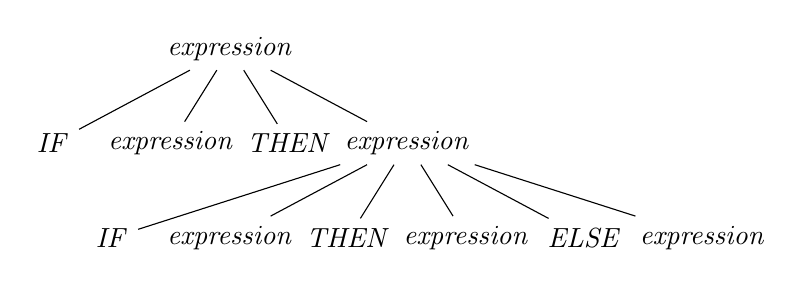
\begin{tikzpicture}[level distance=12mm]
\node { \nt{expression} }
  child { node {\basic{IF}} }
  child { node {\nt{expression}} }
  child { node {\basic{THEN}} }
  child { node {\nt{expression}}
    child { node {\basic{IF}} }
    child { node {\nt{expression}} }
    child { node {\basic{THEN}} }
    child { node {\nt{expression}} }
    child { node {\basic{ELSE}} }
    child { node {\nt{expression}} }
  }
;
\end{tikzpicture}
\end{heveapicture}
\end{center}
\caption{A partial derivation tree that justifies shifting}
\label{fig:shifting:tree}
\end{figure}

\begin{figure}
\begin{center}
\begin{tabbing}
\= \nt{expression} \\
\> \basic{IF} \nt{expression} \basic{THEN} \= \nt{expression} \\
\>                                         \> \basic{IF} \nt{expression} \basic{THEN} \basic{expression}
                                              . \basic{ELSE} \nt{expression}
\end{tabbing}
\end{center}
\caption{A textual version of the tree in \fref{fig:shifting:tree}}
\label{fig:shifting:text}
\end{figure}

In our example, the proof that shifting is possible is the derivation tree
shown in Figures~\ref{fig:shifting:tree} and~\ref{fig:shifting:text}. At the
root of the tree is the grammar's start symbol, \nt{expression}. This symbol
develops into the string \nt{IF expression THEN expression}, which forms the
tree's second level. The second occurrence of \nt{expression} in that string
develops into \nt{IF expression THEN expression ELSE expression}, which forms
the tree's last level. The tree's fringe, a sentential form, is the string
\nt{IF expression THEN IF expression THEN expression ELSE expression}. As
announced earlier, it begins with the conflict string \nt{IF expression THEN
IF expression THEN expression}, followed with the conflict token
\nt{ELSE}.

In \fref{fig:shifting:text}, the end of the conflict string is materialized
with a dot. Note that this dot does not occupy the rightmost position in the
tree's last level. In other words, the conflict token (\basic{ELSE}) itself
occurs on the tree's last level. In practical terms, this means that, after
the automaton has recognized the conflict string and peeked at the conflict
token, it makes sense for it to \emph{shift} that token.

\paragraph{Why reducing is legal}

\begin{figure}
\mycommonbaseline
\begin{center}
\begin{heveapicture}
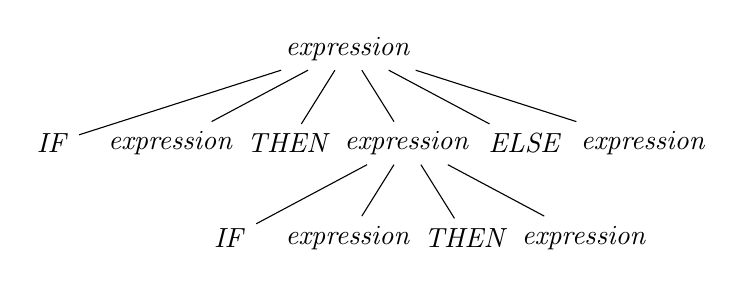
\begin{tikzpicture}[level distance=12mm]
\node { \nt{expression} }
  child { node {\basic{IF}} }
  child { node {\nt{expression}} }
  child { node {\basic{THEN}} }
  child { node {\nt{expression}}
    child { node {\basic{IF}} }
    child { node {\nt{expression}} }
    child { node {\basic{THEN}} }
    child { node {\nt{expression}} }
  }
  child { node {\basic{ELSE}} }
  child { node {\nt{expression}} }
;
\end{tikzpicture}
\end{heveapicture}
\end{center}
\caption{A partial derivation tree that justifies reducing}
\label{fig:reducing:tree}
\end{figure}

\begin{figure}
\begin{center}
\begin{tabbing}
\= \nt{expression} \\
\> \basic{IF} \nt{expression} \basic{THEN} \= \nt{expression} \basic{ELSE} \nt{expression}
                                                              \sidecomment{lookahead token appears} \\
\>                                         \> \basic{IF} \nt{expression} \basic{THEN} \basic{expression} .
\end{tabbing}
\end{center}
\caption{A textual version of the tree in \fref{fig:reducing:tree}}
\label{fig:reducing:text}
\end{figure}

In our example, the proof that reducing is possible is the derivation tree
shown in Figures~\ref{fig:reducing:tree} and~\ref{fig:reducing:text}. Again,
the sentential form found at the fringe of the tree begins with the conflict
string, followed with the conflict token.

Again, in \fref{fig:reducing:text}, the end of the conflict string is
materialized with a dot. Note that, this time, the dot occupies the rightmost
position in the tree's last level. In other words, the conflict token
(\basic{ELSE}) appeared on an earlier level (here, on the second level).  This
fact is emphasized by the comment \inlinesidecomment{lookahead token appears}
found at the second level. In practical terms, this means that, after the
automaton has recognized the conflict string and peeked at the conflict token,
it makes sense for it to \emph{reduce} the production that corresponds to the
tree's last level---here, the production is \nt{expression} $\rightarrow$
\basic{IF} \nt{expression} \basic{THEN} \basic{expression}.

\paragraph{An example of a more complex derivation tree}

Figures~\ref{fig:xreducing:tree} and~\ref{fig:xreducing:text} show a partial
derivation tree that justifies reduction in a more complex situation. (This
derivation tree is relative to a grammar that is not shown.) Here, the
conflict string is \basic{DATA UIDENT EQUALS UIDENT}; the conflict token is
\basic{LIDENT}.  It is quite clear that the fringe of the tree begins with the
conflict string.  However, in this case, the fringe does not explicitly
exhibit the conflict token. Let us examine the tree more closely and answer
the question: following \basic{UIDENT}, what's the next terminal symbol on the
fringe?

\begin{figure}
\mycommonbaseline
\begin{center}
\begin{heveapicture}
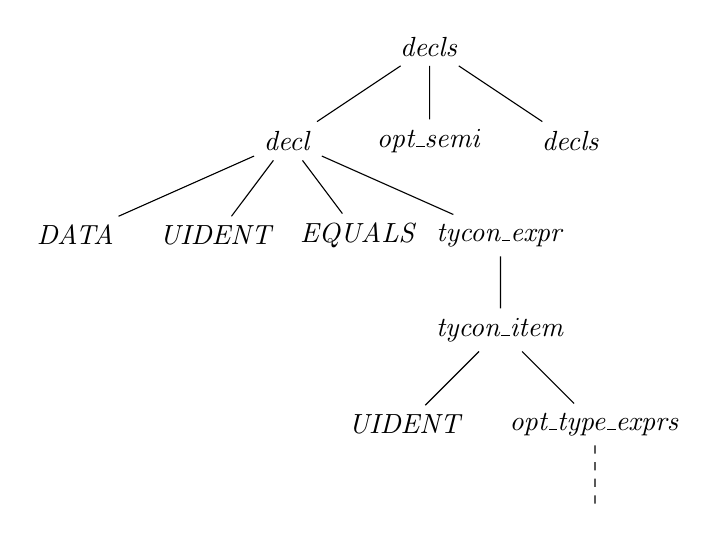
\begin{tikzpicture}[level distance=12mm,level 1/.style={sibling distance=18mm},
                                        level 2/.style={sibling distance=18mm},
                                        level 4/.style={sibling distance=24mm}]]
\node { \nt{decls} }
  child { node {\nt{decl}}
    child { node {\basic{DATA}} }
    child { node {\basic{UIDENT}} }
    child { node {\basic{EQUALS}} }
    child { node {\nt{tycon\_expr}}
      child { node {\nt{tycon\_item}}
        child { node {\basic{UIDENT}} }
        child { node {\nt{opt\_type\_exprs}}
          child { node {} edge from parent [dashed] }
        }
      }
    }
  }
  child { node {\nt{opt\_semi}} }
  child { node {\nt{decls}} }
;
\end{tikzpicture}
\end{heveapicture}
\end{center}
\caption{A partial derivation tree that justifies reducing}
\label{fig:xreducing:tree}
\end{figure}

\begin{figure}
\begin{center}
\begin{tabbing}
\= \nt{decls} \\
\> \nt{decl} \nt{opt\_semi} \nt{decls}
\sidecomment{lookahead token appears because \nt{opt\_semi} can vanish
   and \nt{decls} can begin with \basic{LIDENT}} \\
\> \basic{DATA UIDENT} \basic{EQUALS} \= \nt{tycon\_expr}
\sidecomment{lookahead token is inherited} \\
\> \> \nt{tycon\_item} \sidecomment{lookahead token is inherited} \\
\> \> \basic{UIDENT} \= \nt{opt\_type\_exprs} \sidecomment{lookahead token is inherited} \\
\> \> \> .
\end{tabbing}
\end{center}
\caption{A textual version of the tree in \fref{fig:xreducing:tree}}
\label{fig:xreducing:text}
\end{figure}
% TEMPORARY the HTML rendering of this figure isn't good

First, note that \nt{opt\_type\_exprs} is \emph{not} a leaf node, even though
it has no children. The grammar contains the production $\nt{opt\_type\_exprs}
\rightarrow \epsilon$: the nonterminal symbol \nt{opt\_type\_exprs} develops
to the empty string. (This is made clear in \fref{fig:xreducing:text}, where a
single dot appears immediately below \nt{opt\_type\_exprs}.) Thus,
\nt{opt\_type\_exprs} is not part of the fringe.

Next, note that \nt{opt\_type\_exprs} is the rightmost symbol within its
level. Thus, in order to find the next symbol on the fringe, we have to look
up one level. This is the meaning of the comment \inlinesidecomment{lookahead
token is inherited}. Similarly, \nt{tycon\_item} and \nt{tycon\_expr} appear
rightmost within their level, so we again have to look further up.

This brings us back to the tree's second level. There, \nt{decl} is \emph{not}
the rightmost symbol: next to it, we find \nt{opt\_semi} and \nt{decls}. Does
this mean that \nt{opt\_semi} is the next symbol on the fringe? Yes and no.
\nt{opt\_semi} is a \emph{nonterminal} symbol, but we are really interested in finding
out what the next \emph{terminal} symbol on the fringe could be. The partial
derivation tree shown in Figures~\ref{fig:xreducing:tree}
and~\ref{fig:xreducing:text} does not explicitly answer this question. In
order to answer it, we need to know more about \nt{opt\_semi} and \nt{decls}.

Here, \nt{opt\_semi} stands (as one might have guessed) for an optional
semicolon, so the grammar contains a production $\nt{opt\_semi} \rightarrow
\epsilon$. This is indicated by the comment
\inlinesidecomment{\nt{opt\_semi} can vanish}. (Nonterminal symbols
that generate $\epsilon$ are also said to be \emph{nullable}.) Thus, one could
choose to turn this partial derivation tree into a larger one by developing
\nt{opt\_semi} into $\epsilon$, making it a non-leaf node. That would yield
a new partial derivation tree where the next symbol on the fringe, following
\basic{UIDENT}, is \nt{decls}.

Now, what about \nt{decls}? Again, it is a \emph{nonterminal} symbol, and we
are really interested in finding out what the next \emph{terminal} symbol on
the fringe could be. Again, we need to imagine how this partial derivation
tree could be turned into a larger one by developing \nt{decls}. Here, the
grammar happens to contain a production of the form $\nt{decls} \rightarrow
\basic{LIDENT} \ldots$ This is indicated by the comment
\inlinesidecomment{\nt{decls} can begin with \basic{LIDENT}}.
Thus, by developing \nt{decls}, it is possible to construct a partial
derivation tree where the next symbol on the fringe, following
\basic{UIDENT}, is \basic{LIDENT}. This is precisely the conflict
token.

To sum up, there exists a partial derivation tree whose
fringe begins with the conflict string, followed with the conflict token.
Furthermore, in that derivation tree, the dot occupies the rightmost position
in the last level. As in our previous example, this means that, after the
automaton has recognized the conflict string and peeked at the conflict token,
it makes sense for it to \emph{reduce} the production that corresponds to the
tree's last level---here, the production is $\nt{opt\_type\_exprs}
\rightarrow \epsilon$.

\paragraph{Greatest common factor among derivation trees}

Understanding conflicts requires comparing two (or more) derivation trees. It
is frequent for these trees to exhibit a common factor, that is, to exhibit
identical structure near the top of the tree, and to differ only below a
specific node. Manual identification of that node can be tedious, so \menhir
performs this work automatically. When explaining a $n$-way conflict, it first
displays the greatest common factor of the $n$ derivation trees. A question
mark symbol $\basic{(?)}$ is used to identify the node where the trees begin
to differ. Then, \menhir displays each of the $n$ derivation trees,
\emph{without their common factor} -- that is, it displays $n$ sub-trees that
actually begin to differ at the root. This should make visual comparisons
significantly easier.

\subsection{How are severe conflicts resolved in the end?}

It is unspecified how severe conflicts are resolved. \menhir attempts to mimic
\ocamlyacc's specification, that is, to resolve shift/reduce conflicts in favor
of shifting, and to resolve reduce/reduce conflicts in favor of the production
that textually appears earliest in the grammar specification. However, this
specification is inconsistent in case of three-way conflicts, that is,
conflicts that simultaneously involve a shift action and several reduction
actions. Furthermore, textual precedence can be undefined when the grammar
specification is split over multiple modules. In short, \menhir's philosophy is
that
\begin{center}
severe conflicts should not be tolerated,
\end{center}
so you should not care how they are resolved.

% If a shift/reduce conflict is resolved in favor of reduction, then there can
% exist words of terminal symbols that are accepted by the canonical LR(1)
% automaton without traversing any conflict state and which are rejected by our
% automaton (constructed by Pager's method followed by conflict
% resolution). Same problem when a shift/reduce conflict is resolved in favor of
% neither action (via \dnonassoc) or when a reduce/reduce conflict is resolved
% arbitrarily.

\subsection{End-of-stream conflicts}
\label{sec:eos}

\menhir's treatment of the end of the token stream is (believed to be) fully compatible
with \ocamlyacc's. Yet, \menhir attempts to be more user-friendly by warning
about a class of so-called ``end-of-stream conflicts''.

% TEMPORARY il faut noter que \menhir n'est pas conforme à ocamlyacc en
% présence de conflits end-of-stream; apparemment il part dans le mur
% en exigeant toujours le token suivant, alors que ocamlyacc est capable
% de s'arrêter (comment?); cf. problème de S. Hinderer (avril 2015).

\paragraph{How the end of stream is handled}

In many textbooks on parsing, it is assumed that the lexical analyzer, which
produces the token stream, produces a special token, written \eos, to signal
that the end of the token stream has been reached. A parser generator can take
advantage of this by transforming the grammar: for each start symbol $\nt{S}$
in the original grammar, a new start symbol $\nt{S'}$ is defined, together
with the production $S'\rightarrow S\eos$. The symbol $S$ is no longer a start
symbol in the new grammar. This means that the parser will accept a sentence
derived from $S$ only if it is immediately followed by the end of the token
stream.

This approach has the advantage of simplicity. However, \ocamlyacc and \menhir
do not follow it, for several reasons. Perhaps the most convincing one is that
it is not flexible enough: sometimes, it is desirable to recognize a sentence
derived from $S$, \emph{without} requiring that it be followed by the end of
the token stream: this is the case, for instance, when reading commands, one
by one, on the standard input channel. In that case, there is no end of stream:
the token stream is conceptually infinite. Furthermore, after a command has
been recognized, we do \emph{not} wish to examine the next token, because
doing so might cause the program to block, waiting for more input.

In short, \ocamlyacc and \menhir's approach is to recognize a sentence derived
from $S$ and to \emph{not look}, if possible, at what follows. However, this
is possible only if the definition of $S$ is such that the end of an
$S$-sentence is identifiable without knowledge of the lookahead token. When
the definition of $S$ does not satisfy this criterion, and \emph{end-of-stream
conflict} arises: after a potential $S$-sentence has been read, there can be a
tension between consulting the next token, in order to determine whether the
sentence is continued, and \emph{not} consulting the next token, because the
sentence might be over and whatever follows should not be read. \menhir warns
about end-of-stream conflicts, whereas \ocamlyacc does not.

\paragraph{A definition of end-of-stream conflicts}

Technically, \menhir proceeds as follows. A \eos symbol is introduced. It is,
however, only a \emph{pseudo-}token: it is never produced by the lexical
analyzer. For each start symbol $\nt{S}$ in the original grammar, a new start
symbol $\nt{S'}$ is defined, together with the production $S'\rightarrow S$.
The corresponding start state of the LR(1) automaton is composed of the LR(1)
item $S' \rightarrow . \;S\; [\eos]$. That is, the pseudo-token \eos initially
appears in the lookahead set, indicating that we expect to be done after
recognizing an $S$-sentence. During the construction of the LR(1) automaton,
this lookahead set is inherited by other items, with the effect that, in the
end, the automaton has:
\begin{itemize}
\item \emph{shift} actions only on physical tokens; and
\item \emph{reduce} actions either on physical tokens or on the pseudo-token \eos.
\end{itemize}
A state of the automaton has a reduce action on \eos if, in that state, an
$S$-sentence has been read, so that the job is potentially finished. A state
has a shift or reduce action on a physical token if, in that state, more
tokens potentially need to be read before an $S$-sentence is recognized. If a
state has a reduce action on \eos, then that action should be taken
\emph{without} requesting the next token from the lexical analyzer. On the
other hand, if a state has a shift or reduce action on a physical token, then
the lookahead token \emph{must} be consulted in order to determine if that
action should be taken.

\begin{figure}[p]
\begin{quote}
\begin{tabular}{l}
\dtoken \kangle{\basic{int}} \basic{INT} \\
\dtoken \basic{PLUS TIMES} \\
\dleft PLUS \\
\dleft TIMES \\
\dstart \kangle{\basic{int}} \nt{expr} \\
\percentpercent \\
\nt{expr}:
\newprod \basic{i} = \basic{INT} \dpaction{\basic{i}}
\newprod \basic{e1} = \nt{expr} \basic{PLUS} \basic{e2} = \nt{expr} \dpaction{\basic{e1 + e2}}
\newprod \basic{e1} = \nt{expr} \basic{TIMES} \basic{e2} = \nt{expr} \dpaction{\basic{e1 * e2}}
\end{tabular}
\end{quote}
\caption{Basic example of an end-of-stream conflict}
\label{fig:basiceos}
\end{figure}

\begin{figure}[p]
\begin{verbatim}
State 6:
expr -> expr . PLUS expr [ # TIMES PLUS ]
expr -> expr PLUS expr . [ # TIMES PLUS ]
expr -> expr . TIMES expr [ # TIMES PLUS ]
-- On TIMES shift to state 3
-- On # PLUS reduce production expr -> expr PLUS expr

State 4:
expr -> expr . PLUS expr [ # TIMES PLUS ]
expr -> expr . TIMES expr [ # TIMES PLUS ]
expr -> expr TIMES expr . [ # TIMES PLUS ]
-- On # TIMES PLUS reduce production expr -> expr TIMES expr

State 2:
expr' -> expr . [ # ]
expr -> expr . PLUS expr [ # TIMES PLUS ]
expr -> expr . TIMES expr [ # TIMES PLUS ]
-- On TIMES shift to state 3
-- On PLUS shift to state 5
-- On # accept expr
\end{verbatim}
\caption{Part of an LR automaton for the grammar in \fref{fig:basiceos}}
\label{fig:basiceosdump}
\end{figure}

\begin{figure}[p]
\begin{quote}
\begin{tabular}{l}
\ldots \\
\dtoken \basic{END} \\
\dstart \kangle{\basic{int}} \nt{main} \hspace{1cm} \textit{// instead of \nt{expr}} \\
\percentpercent \\
\nt{main}:
\newprod \basic{e} = \nt{expr} \basic{END} \dpaction{\basic{e}} \\
\nt{expr}:
\newprod \ldots
\end{tabular}
\end{quote}
\caption{Fixing the grammar specification in \fref{fig:basiceos}}
\label{fig:basiceos:sol}
\end{figure}

An end-of-stream conflict arises when a state has distinct actions on \eos and
on at least one physical token. In short, this means that the end of an
$S$-sentence cannot be unambiguously identified without examining one extra
token. \menhir's default behavior, in that case, is to suppress the action on
\eos, so that more input is \emph{always} requested.

\paragraph{Example}

\fref{fig:basiceos} shows a grammar that has end-of-stream conflicts.
When this grammar is processed, \menhir warns about these conflicts,
and further warns that \nt{expr} is never accepted. Let us explain.

Part of the corresponding automaton, as described in the \automaton file, is
shown in \fref{fig:basiceosdump}. Explanations at the end of the \automaton
file (not shown) point out that states 6 and 2 have an end-of-stream
conflict. Indeed, both states have distinct actions on \eos and on the
physical token \basic{TIMES}.
%
It is interesting to note that, even though state 4 has actions on \eos and on
physical tokens, it does not have an end-of-stream conflict. This is because
the action taken in state 4 is always to reduce the production $\nt{expr}
\rightarrow \nt{expr}$ \basic{TIMES} \nt{expr}, regardless of the lookahead
token.

By default, \menhir produces a parser where end-of-stream conflicts are
resolved in favor of looking ahead: that is, the problematic reduce actions on
\eos are suppressed. This means, in particular, that the \emph{accept} action
in state 2, which corresponds to reducing the production $\nt{expr}
\rightarrow \nt{expr'}$, is suppressed. This explains why the symbol \nt{expr}
is never accepted: because expressions do not have an unambiguous end marker,
the parser will always request one more token and will never stop.

In order to avoid this end-of-stream conflict, the standard solution is to
introduce a new token, say \basic{END}, and to use it as an end marker for
expressions. The \basic{END} token could be generated by the lexical analyzer
when it encounters the actual end of stream, or it could correspond to a piece
of concrete syntax, say, a line feed character, a semicolon, or an
\texttt{end} keyword. The solution is shown in \fref{fig:basiceos:sol}.

% ------------------------------------------------------------------------------

\section{Positions}
\label{sec:positions}

When an \ocamllex-generated lexical analyzer produces a token, it updates
two fields, named \verb+lex_start_p+ and \verb+lex_curr_p+, in its environment
record, whose type is \verb+Lexing.lexbuf+. Each of these fields holds a value
of type \verb+Lexing.position+. Together, they represent the token's start and
end positions within the text that is being scanned. These fields are read by
\menhir after calling the lexical analyzer, so \textbf{it is the lexical
  analyzer's responsibility} to correctly set these fields.

A position consists
mainly of an offset (the position's \verb+pos_cnum+ field), but also holds
information about the current file name, the current line number, and the
current offset within the current line. (Not all \ocamllex-generated analyzers
keep this extra information up to date. This must be explicitly programmed by
the author of the lexical analyzer.)

\begin{figure}
\begin{center}
\begin{tabular}{@{}l@{\hspace{7.0mm}}l@{}}
\verb+$startpos+ & start position of the first symbol in the production's right-hand side, if there is one; \\&
                   end position of the most recently parsed symbol, otherwise \\
\verb+$endpos+   & end position of the last symbol in the production's right-hand side, if there is one; \\&
                   end position of the most recently parsed symbol, otherwise \\
\verb+$startpos(+ \verb+$+\nt{i} \barre \nt{id} \verb+)+
                 & start position of the symbol named \verb+$+\nt{i} or \nt{id} \\
\verb+$endpos(+ \verb+$+\nt{i} \barre \nt{id} \verb+)+
                 &   end position of the symbol named \verb+$+\nt{i} or \nt{id} \\
\ksymbolstartpos & start position of the leftmost symbol \nt{id} such that
                         \verb+$startpos(+\nt{id}\verb+)+ \verb+!=+\, \verb+$endpos(+\nt{id}\verb+)+; \\&
                         if there is no such symbol, \verb+$endpos+ \\[2mm]
%
\verb+$startofs+ \\
\verb+$endofs+   \\
\verb+$startofs(+ \verb+$+\nt{i} \barre \nt{id} \verb+)+ & same as above, but produce an integer offset instead of a position \\
\verb+$endofs(+ \verb+$+\nt{i} \barre \nt{id} \verb+)+ \\
\verb+$symbolstartofs+ \\[2mm]
%
\verb+$loc+ & stands for the pair \verb+($startpos, $endpos)+ \\
\verb+$loc(+ \nt{id} \verb+)+ & stands for the pair \verb+($startpos(+ \nt{id} \verb+), $endpos(+ \nt{id} \verb+))+ \\
  % $loc($i)$ works too,
  % but is not documented,
  % as that would be visually heavy
  % and its use is not encouraged anyway.
\verb+$sloc+ & stands for the pair \verb+($symbolstartpos, $endpos)+ \\
\end{tabular}
\end{center}
\caption{Position-related keywords}
\label{fig:pos}
\end{figure}

% We could document $endpos($0). Not sure whether that would be a good thing.

\begin{figure}
\begin{tabular}{@{}ll@{\hspace{2cm}}l}
% Positions.
\verb+symbol_start_pos()+ &
\ksymbolstartpos          \\
\verb+symbol_end_pos()+   &
\verb+$endpos+            \\
\verb+rhs_start_pos i+    &
\verb+$startpos($i)+      & ($1 \leq i \leq n$) \\
\verb+rhs_end_pos i+      &
\verb+$endpos($i)+        & ($1 \leq i \leq n$) \\ % i = 0 permitted, really
% Offsets.
\verb+symbol_start()+     &
\verb+$symbolstartofs+    \\
\verb+symbol_end()+       &
\verb+$endofs+            \\
\verb+rhs_start i+        &
\verb+$startofs($i)+      & ($1 \leq i \leq n$) \\
\verb+rhs_end i+          &
\verb+$endofs($i)+        & ($1 \leq i \leq n$) \\ % i = 0 permitted, really
\end{tabular}
\caption{Translating position-related incantations from \ocamlyacc to \menhir}
\label{fig:pos:mapping}
\end{figure}

This mechanism allows associating pairs of positions with terminal symbols. If
desired, \menhir automatically extends it to nonterminal symbols as well. That
is, it offers a mechanism for associating pairs of positions with terminal or
nonterminal symbols. This is done by making a set of keywords available to
semantic actions (\fref{fig:pos}). These keywords are
\emph{not} available outside of a semantic action:
in particular, they cannot be used within an \ocaml header.

\ocaml's standard library module \texttt{Parsing} is deprecated. The functions
that it offers \emph{can} be called, but will return dummy positions.

We remark that, if the current production has an empty right-hand side, then
\verb+$startpos+ and \verb+$endpos+ are equal, and (by convention) are the end
position of the most recently parsed symbol (that is, the symbol that happens
to be on top of the automaton's stack when this production is reduced). If
the current production has a nonempty right-hand side, then
\verb+$startpos+ is the same as \verb+$startpos($1)+ and
\verb+$endpos+ is the same as \verb+$endpos($+\nt{n}\verb+)+,
where \nt{n} is the length of the right-hand side.

More generally, if the current production has matched a sentence of length
zero, then \verb+$startpos+ and \verb+$endpos+ will be equal, and conversely.
% (provided the lexer is reasonable and never produces a token whose start and
% end positions are equal).

The position \verb+$startpos+ is sometimes ``further towards the left'' than
one would like. For example, in the following production:
\begin{verbatim}
  declaration: modifier? variable { $startpos }
\end{verbatim}
the keyword \verb+$startpos+ represents the start position of the optional
modifier \verb+modifier?+. If this modifier turns out to be absent, then its
start position is (by definition) the end position of the most recently parsed
symbol. This may not be what is desired: perhaps the user would prefer in this
case to use the start position of the symbol \verb+variable+. This is achieved by
using \ksymbolstartpos instead of \verb+$startpos+. By definition,
\ksymbolstartpos is the start position of the leftmost symbol whose
start and end positions differ. In this example, the computation of
\ksymbolstartpos skips the absent \verb+modifier+, whose start and end
positions coincide, and returns the start position of the symbol \verb+variable+
(assuming this symbol has distinct start and end positions).

% On pourrait souligner que $symbolstartpos renvoie la $startpos du premier
% symbole non vide, et non pas la $symbolstartpos du premier symbole non vide.
% Donc ça peut rester un peu contre-intuitif, et ne pas correspondre
% exactement à ce que l'on attend. D'ailleurs, le calcul de $symbolstartpos
% est préservé par %inline (on obtient cela très facilement en éliminant
% $symbolstartpos avant l'inlining) mais ne correspond pas à ce que donnerait
% $symbolstartpos après un inlining manuel. Fondamentalement, cette notion de
% $symbolstartpos ne tourne pas très rond.

There is no keyword \verb+$symbolendpos+. Indeed, the problem
with \verb+$startpos+ is due to the asymmetry in the definition
of \verb+$startpos+ and \verb+$endpos+ in the case of an empty right-hand
side, and does not affect \verb+$endpos+.

\newcommand{\fineprint}{\footnote{%
    The computation of \ksymbolstartpos
    is optimized by \menhir under two assumptions about the lexer. First,
    \menhir assumes that the lexer never produces a token whose start and end
    positions are equal. Second, \menhir assumes that two positions produced
    by the lexer are equal if and only if they are physically equal. If the
    lexer violates either of these assumptions, the computation of
    \ksymbolstartpos could produce a result that differs from
    \texttt{Parsing.symbol\_start\_pos()}.
}}

The positions computed by \menhir are exactly the same as those computed by
\verb+ocamlyacc+\fineprint. More precisely, \fref{fig:pos:mapping} sums up how
to translate a call to the \texttt{Parsing} module, as used in an \ocamlyacc
grammar, to a \menhir keyword.

We note that \menhir's \verb+$startpos+ does not appear in the right-hand
column in \fref{fig:pos:mapping}. In other words, \menhir's \verb+$startpos+
does not correspond exactly to any of the \ocamlyacc function calls.
An exact \ocamlyacc equivalent of \verb+$startpos+ is \verb+rhs_start_pos 1+
if the current production has a nonempty right-hand side and
\verb+symbol_start_pos()+ if it has an empty right-hand side.

Finally, we remark that \menhir's \dinline keyword (\sref{sec:inline})
does not affect the computation of positions. The same positions are computed,
regardless of where \dinline keywords are placed.

% ------------------------------------------------------------------------------

\section{Using \menhir as an interpreter}
\label{sec:interpret}

When \ointerpret is set, \menhir no longer behaves as a compiler. Instead,
it acts as an interpreter. That is, it repeatedly:
\begin{itemize}
\item reads a sentence off the standard input channel;
\item parses this sentence, according to the grammar;
\item displays an outcome.
\end{itemize}
This process stops when the end of the input channel is reached.

\subsection{Sentences}
\label{sec:sentences}

The syntax of sentences is as follows:
\begin{center}
\begin{tabular}{r@{}c@{}l}
\nt{sentence} \is
  \optional{\nt{lid}\,\deuxpoints} \sepspacelist{\nt{uid}} \,\dnewline
\end{tabular}
\end{center}

Less formally, a sentence is a sequence of zero or more terminal symbols
(\nt{uid}'s), separated with whitespace, terminated with a newline character,
and optionally preceded with a non-terminal start symbol (\nt{lid}). This
non-terminal symbol can be omitted if, and only if, the grammar only has one
start symbol.

For instance, here are four valid sentences for the grammar of arithmetic
expressions found in the directory \distrib{demos/calc}:
%
\begin{verbatim}
main: INT PLUS INT EOL
INT PLUS INT
INT PLUS PLUS INT EOL
INT PLUS PLUS
\end{verbatim}
%
In the first sentence, the start symbol \texttt{main} was explicitly
specified. In the other sentences, it was omitted, which is permitted, because
this grammar has no start symbol other than \texttt{main}.  The first sentence
is a stream of four terminal symbols, namely \texttt{INT}, \texttt{PLUS},
\texttt{INT}, and \texttt{EOL}. These terminal symbols must be provided under
their symbolic names. Writing, say, ``\texttt{12+32\textbackslash n}'' instead
of \texttt{INT PLUS INT EOL} is not permitted. \menhir would not be able to
make sense of such a concrete notation, since it does not have a lexer for it.

% On pourrait documenter le fait qu'une phrase finie est transformée par \menhir
% en un flot de tokens potentiellement infinie, avec un suffixe infini EOF ...
% Mais c'est un hack, qui pourrait changer à l'avenir.

\subsection{Outcomes}
\label{sec:outcomes}

As soon as \menhir is able to read a complete sentence off the standard input
channel (that is, as soon as it finds the newline character that ends the
sentence), it parses the sentence according to whichever grammar was specified
on the command line, and displays an outcome.

An outcome is one of the following:
\begin{itemize}
\item \texttt{ACCEPT}: a prefix of the sentence was successfully parsed;
      a parser generated by \menhir would successfully stop and produce
      a semantic value;
\item \texttt{OVERSHOOT}: the end of the sentence was reached before it
      could be accepted; a parser generated by \menhir would request a
      non-existent ``next token'' from the lexer, causing it to fail or
      block;
\item \texttt{REJECT}: the sentence was not accepted; a parser generated
      by \menhir would raise the exception \texttt{Error}.
\end{itemize}

When \ointerpretshowcst is set, each \texttt{ACCEPT} outcome is followed with
a concrete syntax tree. A concrete syntax tree is either a leaf or a node.  A
leaf is either a terminal symbol or \error. A node is annotated with a
non-terminal symbol, and carries a sequence of immediate descendants that
correspond to a valid expansion of this non-terminal symbol. \menhir's
notation for concrete syntax trees is as follows:
\begin{center}
\begin{tabular}{r@{}c@{}l}
\nt{cst} \is
   \nt{uid} \\
&& \error \\
&& \texttt{[} \nt{lid}\,\deuxpoints \sepspacelist{\nt{cst}} \texttt{]}
\end{tabular}
\end{center}

% This notation is not quite unambiguous (it is ambiguous if several
% productions are identical).

For instance, if one wished to parse the example sentences of
\sref{sec:sentences} using the grammar of arithmetic expressions in
\distrib{demos/calc}, one could invoke \menhir as follows:
\begin{verbatim}
$ menhir --interpret --interpret-show-cst demos/calc/parser.mly
main: INT PLUS INT EOL
ACCEPT
[main: [expr: [expr: INT] PLUS [expr: INT]] EOL]
INT PLUS INT
OVERSHOOT
INT PLUS PLUS INT EOL
REJECT
INT PLUS PLUS
REJECT
\end{verbatim}
(Here, \menhir's input---the sentences provided by the user on the standard
input channel--- is shown intermixed with \menhir's output---the outcomes
printed by \menhir on the standard output channel.) The first sentence is
valid, and accepted; a concrete syntax tree is displayed. The second sentence
is incomplete, because the grammar specifies that a valid expansion of
\texttt{main} ends with the terminal symbol \texttt{EOL}; hence, the outcome
is \texttt{OVERSHOOT}. The third sentence is invalid, because of the repeated
occurrence of the terminal symbol \texttt{PLUS}; the outcome is
\texttt{REJECT}. The fourth sentence, a prefix of the third one, is rejected
for the same reason.

\subsection{Remarks}

Using \menhir as an interpreter offers an easy way of debugging your grammar.
For instance, if one wished to check that addition is considered
left-associative, as requested by the \dleft directive found in the file
\distrib{demos/calc/parser.mly}, one could submit the following sentence:
\begin{verbatim}
$ ./menhir --interpret --interpret-show-cst ../demos/calc/parser.mly
INT PLUS INT PLUS INT EOL
ACCEPT
[main:
  [expr: [expr: [expr: INT] PLUS [expr: INT]] PLUS [expr: INT]]
  EOL
]
\end{verbatim}
%$
The concrete syntax tree displayed by \menhir is skewed towards the left,
as desired.

The switches \ointerpret and \otrace can be used in conjunction. When
\otrace is set, the interpreter logs its actions to the standard error
channel.

% ------------------------------------------------------------------------------

\section{Generated API}

When \menhir processes a grammar specification, say \texttt{parser.mly}, it
produces one \ocaml module, \texttt{Parser}, whose code resides in the file
\texttt{parser.ml} and whose signature resides in the file
\texttt{parser.mli}. We now review this signature. For simplicity,
we assume that the grammar specification has just one start symbol
\verb+main+, whose \ocaml type is \verb+thing+.

% ------------------------------------------------------------------------------

\subsection{Monolithic API}
\label{sec:monolithic}

The monolithic API defines the type \verb+token+, the exception \verb+Error+,
and the parsing function \verb+main+, named after the start symbol of the
grammar.

%% type token

The type \verb+token+ is an algebraic data type. A value of type \verb+token+
represents a terminal symbol and its semantic value. For instance, if the
grammar contains the declarations \verb+%token A+ and \verb+%token<int> B+,
then the generated file \texttt{parser.mli} contains the following definition:
\begin{verbatim}
  type token =
  | A
  | B of int
\end{verbatim}
%
If \oonlytokens is specified on the command line, the type \verb+token+ is
generated, and the rest is omitted. On the contrary, if \oexternaltokens is
used, the type \verb+token+ is omitted, but the rest (described below) is
generated.

%% exception Error

The exception \verb+Error+ carries no argument. It is raised by the parsing
function \verb+main+ (described below) when a syntax error is detected.
%
\begin{verbatim}
  exception Error
\end{verbatim}

%% val main

Next comes one parsing function for each start symbol of the grammar. Here, we
have assumed that there is one start symbol, named \verb+main+, so the
generated file \texttt{parser.mli} contains the following declaration:
\begin{verbatim}
  val main: (Lexing.lexbuf -> token) -> Lexing.lexbuf -> thing
\end{verbatim}
% On ne montre pas la définition de l'exception Error.
This function expects two arguments, namely: a lexer, which typically is produced by
\ocamllex and has type \verb+Lexing.lexbuf -> token+; and a lexing buffer,
which has type \verb+Lexing.lexbuf+. This API is compatible with
\ocamlyacc. (For information on using \menhir without \ocamllex, please
consult \sref{sec:qa}.)
%
This API is ``monolithic'' in the sense that there is just one function, which
does everything: it pulls tokens from the lexer, parses, and eventually
returns a semantic value (or fails by throwing the exception \texttt{Error}).

% We may wish to note that the behavior of the function \verb+main+
% is influenced by the strategy that is chosen at compile time via
% \ostrategy.

% ------------------------------------------------------------------------------

\subsection{Incremental API}
\label{sec:incremental}

If \otable is set, \menhir offers an incremental API in addition to the
monolithic API. In this API, control is inverted. The parser does not have
access to the lexer. Instead, when the parser needs the next token, it stops
and returns its current state to the user. The user is then responsible for
obtaining this token (typically by invoking the lexer) and resuming the parser
from that state.
%
The directory \distrib{demos/calc-incremental} contains a demo that
illustrates the use of the incremental API.

This API is ``incremental'' in the sense that the user has access to a
sequence of the intermediate states of the parser. Assuming that semantic
values are immutable, a parser state is a persistent data structure: it can be
stored and used multiple times, if desired. This enables applications such as
``live parsing'', where a buffer is continuously parsed while it is being
edited. The parser can be re-started in the middle of the buffer whenever the
user edits a character. Because two successive parser states share most of
their data in memory, a list of $n$ successive parser states occupies only
$O(n)$ space in memory.

% One could point out that semantic actions should be side-effect free.
% But that is an absolute requirement. Semantic actions can have side
% effects, if the user knows what they are doing.

% TEMPORARY actually, live parsing also requires a way of performing
% error recovery, up to a complete parse... as in Merlin.

% ------------------------------------------------------------------------------

\subsubsection{Starting the parser}

In this API, the parser is started by invoking
\verb+Incremental.main+. (Recall that we assume that \verb+main+ is
the name of the start symbol.) The generated file \texttt{parser.mli} contains
the following declaration:
\begin{verbatim}
  module Incremental : sig
    val main: position -> thing MenhirInterpreter.checkpoint
  end
\end{verbatim}
The argument is the initial position. If the lexer is based on an \ocaml
lexing buffer, this argument should be \verb+lexbuf.lex_curr_p+.
In \sref{sec:incremental} and \sref{sec:inspection},
the type \verb+position+ is a synonym for \verb+Lexing.position+.

We emphasize that the function \verb+Incremental.main+ does not parse
anything. It constructs a checkpoint which serves as a \emph{starting}
point. The functions \verb+offer+ and \verb+resume+, described below, are used
to drive the parser.

% ------------------------------------------------------------------------------

\subsubsection{Driving the parser}
\label{sec:incremental:driving}

The sub-module \menhirinterpreter is also part of the incremental API.
Its declaration, which appears in the generated file \texttt{parser.mli}, is as
follows:
\begin{verbatim}
  module MenhirInterpreter : MenhirLib.IncrementalEngine.INCREMENTAL_ENGINE
    with type token = token
\end{verbatim}
The signature \verb+INCREMENTAL_ENGINE+, defined in the module
\menhirlibincrementalengine, contains many types and functions,
which are described in the rest of this section
(\sref{sec:incremental:driving}) and in the following sections
(\sref{sec:incremental:inspecting}, \sref{sec:incremental:updating}).

Please keep in mind that, from the outside, these types and functions should be referred
to with an appropriate prefix. For instance, the type \verb+checkpoint+ should be referred
to as \verb+MenhirInterpreter.checkpoint+, or
\verb+Parser.MenhirInterpreter.checkpoint+, depending on which modules the user
chooses to open.

%% type token

% Passons-le sous silence.

%% type 'a env

\begin{verbatim}
  type 'a env
\end{verbatim}

The abstract type \verb+'a env+ represents the current state of the
parser. (That is, it contains the current state and stack of the LR
automaton.) Assuming that semantic values are immutable, it is a persistent
data structure: it can be stored and used multiple times, if desired.
The parameter \verb+'a+ is the type of the semantic value that will
eventually be produced if the parser succeeds.

%% type production

\begin{verbatim}
  type production
\end{verbatim}

The abstract type \verb+production+ represents a production of the grammar.
%
The ``start productions'' (which do not exist in an \mly file, but are
constructed by \menhir internally) are \emph{not} part of this type.

%% type 'a checkpoint

\begin{verbatim}
  type 'a checkpoint = private
    | InputNeeded of 'a env
    | Shifting of 'a env * 'a env * bool
    | AboutToReduce of 'a env * production
    | HandlingError of 'a env
    | Accepted of 'a
    | Rejected
\end{verbatim}

The type \verb+'a checkpoint+ represents an intermediate or
final state of the parser. An intermediate checkpoint is a suspension: it records
the parser's current state, and allows parsing to be resumed. The parameter
\verb+'a+ is the type of the semantic value that will eventually be produced
if the parser succeeds.

\verb+Accepted+ and \verb+Rejected+ are final checkpoints. \verb+Accepted+ carries
a semantic value.

\verb+InputNeeded+ is an intermediate checkpoint. It means that the parser wishes
to read one token before continuing.

\verb+Shifting+ is an intermediate checkpoint. It means that the parser is taking
a shift transition. It exposes the state of the parser before and after the
transition. The Boolean parameter tells whether the parser intends to request
a new token after this transition. (It always does, except when it is about to
accept.)

\verb+AboutToReduce+ is an intermediate checkpoint: it means that the parser is
about to perform a reduction step. \verb+HandlingError+ is also an
intermediate checkpoint: it means that the parser has detected an error and is
about to handle it. (Error handling is typically performed in several steps,
so the next checkpoint is likely to be \verb+HandlingError+ again.) In these two
cases, the parser does not need more input. The parser suspends itself at this
point only in order to give the user an opportunity to observe the parser's
transitions and possibly handle errors in a different manner, if desired.

%% val offer

\begin{verbatim}
  val offer:
    'a checkpoint ->
    token * position * position ->
    'a checkpoint
\end{verbatim}

The function \verb+offer+ allows the user to resume the parser after the
parser has suspended itself with a checkpoint of the form \verb+InputNeeded env+.
This function expects the previous checkpoint \verb+checkpoint+ as well as a new token
(together with the start and end positions of this token). It produces a new
checkpoint, which again can be an intermediate checkpoint or a final checkpoint. It does
not raise any exception. (The exception \texttt{Error} is used only in the
monolithic API.)

%% val resume

\begin{verbatim}
  val resume:
    ?strategy:[ `Legacy | `Simplified ] ->
    'a checkpoint ->
    'a checkpoint
\end{verbatim}

The function \verb+resume+ allows the user to resume the parser after the
parser has suspended itself with a checkpoint of the form
\verb+AboutToReduce (env, prod)+ or \verb+HandlingError env+.
This function expects just the previous checkpoint \verb+checkpoint+. It produces a new
checkpoint. It does not raise any exception.
%
The optional argument \verb+strategy+ influences the manner in which
\verb+resume+ deals with checkpoints of the form \verb+ErrorHandling _+. Its
default value is \verb+`Legacy+. For more details, see \sref{sec:errors}.

The incremental API subsumes the monolithic API. Indeed, \verb+main+ can be
(and is in fact) implemented by first using
\verb+Incremental.main+, then calling \verb+offer+ and
\verb+resume+ in a loop, until a final checkpoint is obtained.

%% type supplier

\begin{verbatim}
  type supplier =
    unit -> token * position * position
\end{verbatim}

A token supplier is a function of no arguments which delivers a new token
(together with its start and end positions) every time it is called. The
function \verb+loop+ and its variants, described below, expect a supplier
as an argument.

%% val lexer_lexbuf_to_supplier

\begin{verbatim}
  val lexer_lexbuf_to_supplier:
    (Lexing.lexbuf -> token) -> Lexing.lexbuf -> supplier
\end{verbatim}

The function \verb+lexer_lexbuf_to_supplier+, applied to a lexer and to a
lexing buffer, produces a fresh supplier.

%% (remark about the loop* functions)

The functions \verb+offer+ and \verb+resume+, documented above, are sufficient
to write a parser loop. One can imagine many variations of such a loop, which
is why we expose \verb+offer+ and \verb+resume+ in the first place.
Nevertheless, some variations are so common that it is worth providing them,
ready for use. The following functions are implemented on top of \verb+offer+
and \verb+resume+.

%% val loop

\begin{verbatim}
  val loop:
    ?strategy:[ `Legacy | `Simplified ] ->
    supplier -> 'a checkpoint -> 'a
\end{verbatim}

\verb+loop supplier checkpoint+ begins parsing from \verb+checkpoint+, reading
tokens from \verb+supplier+. It continues parsing until it reaches a
checkpoint of the form \verb+Accepted v+ or \verb+Rejected+. In the former
case, it returns \verb+v+. In the latter case, it raises the
exception \verb+Error+. (By the way, this is how we implement the monolithic
API on top of the incremental API.)
%
The optional argument \verb+strategy+ influences the manner in which
\verb+loop+ deals with checkpoints of the form \verb+ErrorHandling _+. Its
default value is \verb+`Legacy+. For more details, see \sref{sec:errors}.

\begin{verbatim}
  val loop_handle:
    ('a -> 'answer) ->
    ('a checkpoint -> 'answer) ->
    supplier -> 'a checkpoint -> 'answer
\end{verbatim}

\verb+loop_handle succeed fail supplier checkpoint+ begins parsing from
\verb+checkpoint+, reading tokens from \verb+supplier+. It continues until
it reaches a checkpoint of the form \verb+Accepted v+ or \verb+HandlingError _+
(or~\verb+Rejected+, but that should not happen, as \verb+HandlingError _+
will be observed first). In the former case, it calls \verb+succeed v+. In
the latter case, it calls \verb+fail+ with this checkpoint. It cannot
raise \verb+Error+.

This means that \menhir's traditional error-handling procedure (which pops the
stack until a state that can act on the \error token is found) does not get a
chance to run. Instead, the user can implement her own error handling code, in
the \verb+fail+ continuation.

%% val loop_handle_undo

\begin{verbatim}
  val loop_handle_undo:
    ('a -> 'answer) ->
    ('a checkpoint -> 'a checkpoint -> 'answer) ->
    supplier -> 'a checkpoint -> 'answer
\end{verbatim}

\verb+loop_handle_undo+ is analogous to \verb+loop_handle+, but passes a pair
of checkpoints (instead of a single checkpoint) to the failure continuation.
%
The first (and oldest) checkpoint that is passed to the failure continuation
is the last \verb+InputNeeded+ checkpoint that was encountered before the
error was detected. The second (and newest) checkpoint is where the error was
detected. (This is the same checkpoint that \verb+loop_handle+ would pass to
its failure continuation.) Going back to the first checkpoint can be thought
of as undoing any reductions that were performed after seeing the problematic
token. (These reductions must be default reductions or spurious reductions.)
This can be useful to someone who wishes to implement an error explanation or
error recovery mechanism.

\verb+loop_handle_undo+ must be applied to an \verb+InputNeeded+ checkpoint.
The initial checkpoint produced by \verb+Incremental.main+ is of this form.

%% val shifts

\begin{verbatim}
  val shifts: 'a checkpoint -> 'a env option
\end{verbatim}

\verb+shifts checkpoint+ assumes that \verb+checkpoint+ has been obtained by
submitting a token to the parser. It runs the parser from \verb+checkpoint+,
through an arbitrary number of reductions, until the parser either accepts
this token (i.e., shifts) or rejects it (i.e., signals an error). If the
parser decides to shift, then \verb+Some env+ is returned, where \verb+env+ is
the parser's state just before shifting. Otherwise, \verb+None+ is returned.
This can be used to test whether the parser is willing to accept a certain
token. This function should be used with caution, though, as it causes
semantic actions to be executed. It is desirable that all semantic actions be
side-effect-free, or that their side-effects be harmless.

%% val acceptable

\begin{verbatim}
  val acceptable: 'a checkpoint -> token -> position -> bool
\end{verbatim}

\verb+acceptable checkpoint token pos+ requires \verb+checkpoint+ to be an
\verb+InputNeeded+ checkpoint. It returns \verb+true+ iff the parser is
willing to shift this token.
%
This can be used to test, after an error has been detected, which tokens would
have been accepted at this point. To do this, one would typically use
\verb+loop_handle_undo+ to get access to the last \verb+InputNeeded+
checkpoint that was encountered before the error was detected, and apply
\verb+acceptable+ to that checkpoint.

\verb+acceptable+ is implemented using \verb+shifts+, so, like \verb+shifts+,
it causes certain semantic actions to be executed. It is desirable that all
semantic actions be side-effect-free, or that their side-effects be harmless.

% ------------------------------------------------------------------------------

\subsubsection{Inspecting the parser's state}
\label{sec:incremental:inspecting}

Although the type \verb+env+ is opaque, a parser state can be inspected via a
few accessor functions, which are described in this section. The following
types and functions are contained in the \verb+MenhirInterpreter+ sub-module.

%% type 'a lr1state

\begin{verbatim}
  type 'a lr1state
\end{verbatim}

The abstract type \verb+'a lr1state+ describes a (non-initial) state of the
LR(1) automaton.
%
If \verb+s+ is such a state, then \verb+s+ should have at least one incoming
transition, and all of its incoming transitions carry the same (terminal or
non-terminal) symbol, say $A$. We say that $A$ is the \emph{incoming symbol}
of the state~\verb+s+.
%
The index \verb+'a+ is the type of the semantic values associated with $A$.
The role played by \verb+'a+ is clarified in the definition of the
type \verb+element+, which appears further on.

%% val number

\begin{verbatim}
  val number: _ lr1state -> int
\end{verbatim}

The states of the LR(1) automaton are numbered (from 0 and up).
The function \verb+number+ maps a state to its number.

%% val production_index
%% val find_production

\begin{verbatim}
  val production_index: production -> int
  val find_production: int -> production
\end{verbatim}

Productions are numbered. (The set of indices of all productions forms an
interval, which does \emph{not} necessarily begin at 0.)
%
The function \verb+production_index+ converts a production to an integer
number, whereas the function \verb+find_production+ carries out the reverse
conversion. It is an error to apply \verb+find_production+ to an invalid
index.

%% type element

\begin{verbatim}
  type element =
    | Element: 'a lr1state * 'a * position * position -> element
\end{verbatim}

The type \verb+element+ describes one entry in the stack of the LR(1)
automaton. In a stack element of the form \verb+Element (s, v, startp, endp)+,
\verb+s+ is a (non-initial) state and \verb+v+ is a semantic value. The
value~\verb+v+ is associated with the incoming symbol~$A$ of the
state~\verb+s+. In other words, the value \verb+v+ was pushed onto the stack
just before the state \verb+s+ was entered. Thus, for some type \verb+'a+, the
state~\verb+s+ has type \verb+'a lr1state+ and the value~\verb+v+ has
type~\verb+'a+. The positions \verb+startp+ and \verb+endp+ delimit the
fragment of the input text that was reduced to the symbol $A$.

In order to do anything useful with the value \verb+v+, one must gain
information about the type \verb+'a+, by inspection of the state~\verb+s+. So
far, the type \verb+'a lr1state+ is abstract, so there is no way of
inspecting~\verb+s+. The inspection API (\sref{sec:inspection}) offers further
tools for this purpose.

%% val top

\begin{verbatim}
  val top: 'a env -> element option
\end{verbatim}

\verb+top env+ returns the parser's top stack element. The state contained in
this stack element is the current state of the automaton. If the stack is
empty, \verb+None+ is returned. In that case, the current state of the
automaton must be an initial state.

%% val pop_many

\begin{verbatim}
  val pop_many: int -> 'a env -> 'a env option
\end{verbatim}

\verb+pop_many i env+ pops \verb+i+ elements off the automaton's stack. This
is done via \verb+i+ successive invocations of \verb+pop+. Thus,
\verb+pop_many 1+ is \verb+pop+. The index \verb+i+ must be nonnegative. The
time complexity is $O(i)$.

%% val get

\begin{verbatim}
  val get: int -> 'a env -> element option
\end{verbatim}

\verb+get i env+ returns the parser's \verb+i+-th stack element. The index
\verb+i+ is 0-based: thus, \verb+get 0+ is \verb+top+. If \verb+i+ is greater
than or equal to the number of elements in the stack, \verb+None+ is returned.
\verb+get+ is implemented using \verb+pop_many+ and \verb+top+: its time
complexity is $O(i)$.

%% val current_state_number

\begin{verbatim}
  val current_state_number: 'a env -> int
\end{verbatim}

\verb+current_state_number env+ is the integer number of the automaton's
current state. Although this number might conceivably be obtained via the
functions~\verb+top+ and \verb+number+, using \verb+current_state_number+ is
preferable, because this method works even when the automaton's stack is empty
(in which case the current state is an initial state, and \verb+top+ returns
\verb+None+). This number can be passed as an argument to a \verb+message+
function generated by \verb+menhir --compile-errors+.

%% val equal

\begin{verbatim}
  val equal: 'a env -> 'a env -> bool
\end{verbatim}

\verb+equal env1 env2+ tells whether the parser configurations \verb+env1+ and
\verb+env2+ are equal in the sense that the automaton's current state is the
same in \verb+env1+ and \verb+env2+ and the stack is \emph{physically} the
same in \verb+env1+ and \verb+env2+. If \verb+equal env1 env2+ is \verb+true+,
then the sequence of the stack elements, as observed via \verb+pop+ and
\verb+top+, must be the same in \verb+env1+ and \verb+env2+. Also, if
\verb+equal env1 env2+ holds, then the checkpoints \verb+input_needed env1+
and \verb+input_needed env2+ must be equivalent. (The function
\verb+input_needed+ is documented in \sref{sec:incremental:updating}.)
The function \verb+equal+ has time complexity $O(1)$.

%% val positions

\begin{verbatim}
  val positions: 'a env -> position * position
\end{verbatim}

The function \verb+positions+ returns the start and end positions of the
current lookahead token. If invoked in an initial state, this function returns
a pair of twice the initial position that was passed as an argument
to \verb+main+.

%% val has_default_reduction
%% val state_has_default_reduction

\begin{verbatim}
  val env_has_default_reduction: 'a env -> bool
  val state_has_default_reduction: _ lr1state -> bool
\end{verbatim}

When applied to an environment \verb+env+ taken from a checkpoint of the form
\verb+AboutToReduce (env, prod)+, the function
\verb+env_has_default_reduction+ tells whether the reduction that is about to
take place is a default reduction.

\verb+state_has_default_reduction s+ tells whether the state \verb+s+ has a default
reduction. This includes the case where \verb+s+ is an accepting state.

% ------------------------------------------------------------------------------

\subsubsection{Updating the parser's state}
\label{sec:incremental:updating}

The functions presented in the previous section
(\sref{sec:incremental:inspecting}) allow inspecting parser states of type
\verb+'a checkpoint+ and \verb+'a env+. However, so far, there are no
functions for manufacturing new parser states, except \verb+offer+ and
\verb+resume+, which create new checkpoints by feeding tokens, one by one, to
the parser.

In this section, a small number of functions are provided for manufacturing
new parser states of type \verb+'a env+ and \verb+'a checkpoint+. These
functions allow going far back into the past and jumping ahead into the
future, so to speak. In other words, they allow driving the parser in other
ways than by feeding tokens into it. The functions \verb+pop+,
\verb+force_reduction+ and \verb+feed+ (part of the inspection API; see
\sref{sec:inspection}) construct values of type \verb+'a env+. The function
\verb+input_needed+ constructs values of type \verb+'a checkpoint+ and thereby
allows resuming parsing in normal mode (via \verb+offer+). Together, these
functions can be used to implement error handling and error recovery
strategies.

%% val pop

\begin{verbatim}
  val pop: 'a env -> 'a env option
\end{verbatim}

\verb+pop env+ returns a new environment, where the parser's top stack cell
has been popped off. (If the stack is empty, \verb+None+ is returned.) This
amounts to pretending that the (terminal or nonterminal) symbol that
corresponds to this stack cell has not been read.

%% val force_reduction

\begin{verbatim}
  val force_reduction: production -> 'a env -> 'a env
\end{verbatim}

\verb+force_reduction prod env+ can be called only if in the state \verb+env+
the parser is capable of reducing the production \verb+prod+. If this
condition is satisfied, then this production is reduced, which means that its
semantic action is executed (this can have side effects!) and the automaton
makes a goto (nonterminal) transition. If this condition is not satisfied, an
\verb+Invalid_argument+ exception is raised.

%% val input_needed

\begin{verbatim}
  val input_needed: 'a env -> 'a checkpoint
\end{verbatim}

\verb+input_needed env+ returns \verb+InputNeeded env+. Thus, out of a parser
state that might have been obtained via a series of calls to the functions
\verb+pop+, \verb+force_reduction+, \verb+feed+, and so on, it produces a
checkpoint, which can be used to resume normal parsing, by supplying this
checkpoint as an argument to \verb+offer+.

This function should be used with some care. It could ``mess up the
lookahead'' in the sense that it allows parsing to resume in an arbitrary
state \verb+s+ with an arbitrary lookahead symbol \verb+t+, even though
\menhir's reachability analysis (which is carried out via the \olisterrors
switch) might well think that it is impossible to reach this particular
configuration. If one is using \menhir's new error reporting facility
(\sref{sec:errors:new}), this could cause the parser to reach an error state
for which no error message has been prepared.

% ------------------------------------------------------------------------------

\subsection{Inspection API}
\label{sec:inspection}

If \oinspection is set, \menhir offers an inspection API in addition to the
monolithic and incremental APIs. (The reason why this is not done by default
is that this requires more tables to be generated, thus making the generated
parser larger.) Like the incremental API, the inspection API is found in the
sub-module \menhirinterpreter. It offers the following types and functions.

%% type _ terminal

The type \verb+'a terminal+ is a generalized algebraic data type (GADT). A
value of type \verb+'a terminal+ represents a terminal symbol (without a
semantic value). The index \verb+'a+ is the type of the semantic values
associated with this symbol. For instance, if the grammar contains the
declarations \verb+%token A+ and \verb+%token<int> B+, then the generated
module \menhirinterpreter contains the following definition:
%
\begin{verbatim}
  type _ terminal =
  | T_A : unit terminal
  | T_B : int terminal
\end{verbatim}
%
The data constructors are named after the terminal symbols, prefixed with ``\verb+T_+''.

%% type _ nonterminal

The type \verb+'a nonterminal+ is also a GADT. A value of type
\verb+'a nonterminal+ represents a nonterminal symbol (without a semantic value). The
index \verb+'a+ is the type of the semantic values associated with this
symbol. For instance, if \verb+main+ is the only nonterminal symbol,
then the generated
module \menhirinterpreter contains the following definition:
%
\begin{verbatim}
  type _ nonterminal =
  | N_main : thing nonterminal
\end{verbatim}
%
The data constructors are named after the nonterminal symbols, prefixed with ``\verb+N_+''.

%% type 'a symbol

The type \verb+'a symbol+
% (an algebraic data type)
is the disjoint union of the types \verb+'a terminal+ and \verb+'a nonterminal+.
In other words, a value of type \verb+'a symbol+ represents a terminal or nonterminal symbol (without
a semantic value).
This type is (always) defined as follows:
%
\begin{verbatim}
  type 'a symbol =
    | T : 'a terminal -> 'a symbol
    | N : 'a nonterminal -> 'a symbol
\end{verbatim}

%% type xsymbol

The type \verb+xsymbol+ is an existentially quantified version of the
type \verb+'a symbol+. It is useful in situations where the index \verb+'a+ is
not statically known. It is (always) defined as follows:
%
\begin{verbatim}
  type xsymbol =
    | X : 'a symbol -> xsymbol
\end{verbatim}

%% type item

The type \verb+item+ describes an LR(0) item, that is, a pair of a production
\verb+prod+ and an index \verb+i+ into the right-hand side of this production.
If the length of the right-hand side is \verb+n+, then \verb+i+ is
comprised between 0 and \verb+n+, inclusive.

\begin{verbatim}
  type item =
      production * int
\end{verbatim}

%% Comparison functions.

The following functions implement total orderings on the types
\verb+_ terminal+, \verb+_ nonterminal+, \verb+xsymbol+,
\verb+production+, and \verb+item+.

\begin{verbatim}
  val compare_terminals: _ terminal -> _ terminal -> int
  val compare_nonterminals: _ nonterminal -> _ nonterminal -> int
  val compare_symbols: xsymbol -> xsymbol -> int
  val compare_productions: production -> production -> int
  val compare_items: item -> item -> int
\end{verbatim}

%% val incoming_symbol

The function \verb+incoming_symbol+ maps a (non-initial) LR(1)
state~\verb+s+ to its incoming symbol, that is, the symbol that the parser
must recognize before it enters the state \verb+s+.
%
\begin{verbatim}
  val incoming_symbol: 'a lr1state -> 'a symbol
\end{verbatim}
%
This function can be used to gain access to the semantic value \verb+v+
in a stack element \verb+Element (s, v, _, _)+. Indeed, by case analysis on the
symbol \verb+incoming_symbol s+, one gains information about the type \verb+'a+,
hence one obtains the ability to do something useful with the value~\verb+v+.

%% val items

The function \verb+items+ maps a (non-initial) LR(1) state~\verb+s+ to its
LR(0) \emph{core}, that is, to the underlying set of LR(0) items. This set
is represented as a list, whose elements appear in an arbitrary order. This
set is \emph{not} closed under $\epsilon$-transitions.
%
\begin{verbatim}
  val items: _ lr1state -> item list
\end{verbatim}

%% val lhs
%% val rhs

The functions \verb+lhs+ and \verb+rhs+ map a production \verb+prod+ to
its left-hand side and right-hand side, respectively. The left-hand side
is always a nonterminal symbol, hence always of the form \verb+N _+. The
right-hand side is a (possibly empty) sequence of (terminal or nonterminal)
symbols.
%
\begin{verbatim}
  val lhs: production -> xsymbol
  val rhs: production -> xsymbol list
\end{verbatim}
%

%% val nullable

The function \verb+nullable+, applied to a non-terminal symbol,
tells whether this symbol is nullable. A nonterminal symbol is nullable if and
only if it produces the empty word $\epsilon$.
%
\begin{verbatim}
  val nullable: _ nonterminal -> bool
\end{verbatim}

%% val first
%% val xfirst

The function call \verb+first nt t+ tells whether the \emph{FIRST} set of the
nonterminal symbol \verb+nt+ contains the terminal symbol \verb+t+. That is,
it returns \verb+true+ if and only if \verb+nt+ produces a word that begins
with \verb+t+. The function \verb+xfirst+ is identical to \verb+first+, except
it expects a first argument of type \verb+xsymbol+ instead of \verb+_ terminal+.
%
\begin{verbatim}
  val first: _ nonterminal -> _ terminal -> bool
  val xfirst: xsymbol -> _ terminal -> bool
\end{verbatim}

%% val foreach_terminal
%% val foreach_terminal_but_error

The function \verb+foreach_terminal+ enumerates the terminal symbols, including the special symbol \error.
The function \verb+foreach_terminal_but_error+ enumerates the terminal symbols, excluding \error.
\begin{verbatim}
  val foreach_terminal:           (xsymbol -> 'a -> 'a) -> 'a -> 'a
  val foreach_terminal_but_error: (xsymbol -> 'a -> 'a) -> 'a -> 'a
\end{verbatim}

%% val feed

\verb+feed symbol startp semv endp env+ causes the parser to consume the
(terminal or nonterminal) symbol \verb+symbol+, accompanied with the semantic
value \verb+semv+ and with the start and end positions \verb+startp+ and
\verb+endp+. Thus, the automaton makes a transition, and reaches a new state.
The stack grows by one cell. This operation is permitted only if the current
state (as determined by \verb+env+) has an outgoing transition labeled with
\verb+symbol+. Otherwise, an \verb+Invalid_argument+ exception is raised.
\begin{verbatim}
  val feed: 'a symbol -> position -> 'a -> position -> 'b env -> 'b env
\end{verbatim}

% TEMPORARY
% document the modules that use the inspection API: Printers
% document MenhirLib.General?
% The directory \distrib{demos/calc-inspection} contains a demo that illustrates the use of the inspection API.
% review it / clean it up!

% ------------------------------------------------------------------------------

\section{Error handling: the traditional way}
\label{sec:errors}

\menhir's traditional error handling mechanism is considered deprecated: although
it is still supported for the time being, it might be removed in the future.
%
We recommend setting up an error handling mechanism using the new tools
offered by \menhir (\sref{sec:errors:new}).

\paragraph{Error handling}

\menhir's error traditional handling mechanism is inspired by that of \yacc and
\ocamlyacc, but is not identical. A special \error token is made available
for use within productions. The LR automaton is constructed exactly as if
\error was a regular terminal symbol. However, \error is never produced
by the lexical analyzer. Instead, when an error is detected, the current
lookahead token is discarded and replaced with the \error token, which becomes
the current lookahead token. At this point, the parser enters \emph{error
handling} mode.
%
In error handling mode, the parser behaves as follows:
\begin{itemize}
\item If the current state has a shift action on the \error token, then this
  action takes place. Under the \legacy strategy, the parser then
  reads the next token and returns to normal mode. Under the
  simplified strategy, it does \emph{not} request the next token, so
  the current token remains \error, and the parser remains in error handling
  mode.
\item If the current state has a reduce action on the \error token, then this
  action takes place. (This behavior differs from that of \yacc and
  \ocamlyacc, which do not reduce on \error. It is somewhat unclear why not.)
  The current token remains \error and the parser remains in error handling
  mode.
\item If the current state has no action on the \error token, then, under the
  simplified strategy, the parser rejects the input. Under the
  \legacy strategy, the parser pops a cell off its stack and remains
  in error handling mode. If the stack is empty, then the parser rejects the
  input.
\end{itemize}

In the monolithic API, the parser rejects the input by raising the exception
\texttt{Error}. This exception carries no information. The position of the
error can be obtained by reading the lexical analyzer's environment record. In
the incremental API, the parser rejects the input by returning the checkpoint
\texttt{Rejected}.

Which strategy should one choose? First, let us note that the difference
between the strategies \legacy and \simplified matters only if the grammar
uses the \error token. The following rule of thumb can be used to select
between them:
\begin{itemize}
\item If the \error token is used only to catch an error and stop, then the
  \simplified strategy should be preferred. (In this this restricted style,
  the \error token always appears at the end of a production, whose semantic
  action raises an exception.)
\item If the \error token is used to survive an error and continue parsing,
  then the legacy strategy should be selected.
\end{itemize}

\paragraph{Error recovery}

\ocamlyacc offers an error recovery mode, which is entered immediately after
an \error token was successfully shifted. In this mode, tokens are repeatedly
taken off the input stream and discarded until an acceptable token is found.
This feature is no longer offered by \menhir.

\paragraph{Error-related keywords}

The following keyword is made available to semantic actions.

When the \verb+$syntaxerror+ keyword is evaluated, evaluation of the semantic
action is aborted, so that the current reduction is abandoned; the current
lookahead token is discarded and replaced with the \error token; and error
handling mode is entered.  Note that there is no mechanism for inserting an
\error token \emph{in front of} the current lookahead token, even though this
might also be desirable.  It is unclear whether this keyword is useful; it
might be suppressed in the future.

% ------------------------------------------------------------------------------

\section{Error handling: the new way}
\label{sec:errors:new}

\menhir's incremental API (\sref{sec:incremental}) allows taking control when
an error is detected. Indeed, as soon as an invalid token is detected, the
parser produces a checkpoint of the form \verb+HandlingError _+. At this
point, if one decides to let the parser proceed, by just
calling \verb+resume+, then \menhir enters its traditional error handling mode
(\sref{sec:errors}). Instead, however, one can decide to take control and
perform error handling or error recovery in any way one pleases. One can, for
instance, build and display a diagnostic message, based on the automaton's
current stack and/or state. Or, one could modify the input stream, by
inserting or deleting tokens, so as to suppress the error, and resume normal
parsing. In principle, the possibilities are endless.

An apparently simple-minded approach to error reporting,
proposed by Jeffery~\cite{jeffery-03} and further explored by
Pottier~\cite{pottier-reachability-cc-2016}, consists in selecting a diagnostic
message (or a template for a diagnostic message) based purely on the current
state of the automaton.

In this approach, one determines, ahead of time, which are the ``error
states'' (that is, the states in which an error can be detected), and one
prepares, for each error state, a diagnostic message. Because state numbers
are fragile (they change when the grammar evolves), an error state is
identified not by its number, but by an input sentence that leads to it: more
precisely, by an input sentence which causes an error to be detected in this
state. Thus, one maintains a set of pairs of an erroneous input sentence and a
diagnostic message.

\menhir defines a file format, the \messages file format,
for representing this information (\sref{sec:messages:format}), and offers a
set of tools for creating, maintaining, and exploiting \messages files
(\sref{sec:messages:tools}). Once one understands these tools, there remains
to write a collection of diagnostic messages, a more subtle task than one
might think (\sref{sec:errors:diagnostics}), and to glue everything together
(\sref{sec:errors:example}).

In this approach to error handling, as in any other approach, one must
understand exactly when (that is, in which states) errors are detected.
This in turn requires understanding how the automaton is constructed.
\menhir's construction technique is not Knuth's canonical LR(1)
technique~\cite{knuth-lr-65}, which is usually too expensive to be practical.
Instead, \menhir \emph{merges} states~\cite{pager-77} and introduces so-called \emph{default
reductions}. These techniques \emph{defer} error detection by allowing
extra reductions to take place before an error is detected.
% Furthermore, \menhir supports \donerrorreduce declarations,
% which also introduce extra reductions.
The impact of these alterations must be taken into account when writing
diagnostic messages (\sref{sec:errors:diagnostics}).

In this approach to error handling, the special \error token is not used. It
should not appear in the grammar. Similarly, the \verb+$syntaxerror+ keyword
should not be used.

% ------------------------------------------------------------------------------

\subsection{The \messages file format}
\label{sec:messages:format}

\paragraph{Definition}

A \messages file is a text file. It is composed of a list of entries. Each
entry consists of one or more input sentences, followed with one or more blank
lines, followed with a message. Two entries are separated by one or more blank
lines. The syntax of an input sentence is described in \sref{sec:sentences}.
A~message is an arbitrary piece of text, but cannot cannot a blank line.

Blank lines are significant: they are used as separators, both between
entries, and (within an entry) between the sentences and the message. Thus,
there cannot be a blank line between two sentences. (If there is one, \menhir
becomes confused and may complain about some word not being ``a known
non-terminal symbol''). There also cannot be a blank line inside a message.

\begin{figure}
\begin{verbatim}
grammar: TYPE UID
# This hand-written comment concerns just the sentence above.
grammar: TYPE OCAMLTYPE UID PREC
# This hand-written comment concerns just the sentence above.

# This hand-written comment concerns both sentences above.

Ill-formed declaration.
Examples of well-formed declarations:
  %type <Syntax.expression> expression
  %type <int> date time
\end{verbatim}
\caption{An entry in a \messages file}
\label{fig:messages:entry}
\end{figure}

\begin{figure}
\begin{verbatim}
grammar: TYPE UID
##
## Ends in an error in state: 1.
##
## declaration -> TYPE . OCAMLTYPE separated_nonempty_list(option(COMMA),
##   strict_actual) [ TYPE TOKEN START RIGHT PUBLIC PERCENTPERCENT PARAMETER
##   ON_ERROR_REDUCE NONASSOC LEFT INLINE HEADER EOF COLON ]
##
## The known suffix of the stack is as follows:
## TYPE
##
# This hand-written comment concerns just the sentence above.
#
grammar: TYPE OCAMLTYPE UID PREC
##
## Ends in an error in state: 5.
##
## strict_actual -> symbol . loption(delimited(LPAREN,separated_nonempty_list
##   (COMMA,strict_actual),RPAREN)) [ UID TYPE TOKEN START STAR RIGHT QUESTION
##   PUBLIC PLUS PERCENTPERCENT PARAMETER ON_ERROR_REDUCE NONASSOC LID LEFT
##   INLINE HEADER EOF COMMA COLON ]
##
## The known suffix of the stack is as follows:
## symbol
##
# This hand-written comment concerns just the sentence above.

# This hand-written comment concerns both sentences above.

Ill-formed declaration.
Examples of well-formed declarations:
  %type <Syntax.expression> expression
  %type <int> date time
\end{verbatim}
\caption{An entry in a \messages file, decorated with auto-generated comments}
\label{fig:messages:entry:decorated}
\end{figure}

As an example, \fref{fig:messages:entry} shows a valid entry, taken
from \menhir's own \messages file. This entry contains two input sentences,
which lead to errors in two distinct states. A single message is associated
with these two error states.

\paragraph{Comments}

Comment lines, which begin with a \verb+#+ character, are ignored everywhere.
However, users who wish to take advantage of \menhir's facility for merging
two \messages files (\sref{sec:messages:merge}) should follow certain
conventions regarding the placement of comments:
\begin{itemize}
\item If a comment concerns a specific sentence and should remain attached
  to this sentence, then it must immediately follow this sentence
  (without a blank line in between).
\item If a comment concerns all sentences in an entry, then it should appear
  between the sentences and the message, with blank lines in between.
\item One should avoid placing comments between two entries, as the merging
  algorithm will not be able to handle them in a satisfactory way.
\end{itemize}

\paragraph{Auto-generated comments}

Several commands, described next (\sref{sec:messages:tools}),
produce \messages files where each input sentence is followed with an
auto-generated comment, marked with \verb+##+. This special comment indicates
in which state the error is detected, and is supposed to help the reader
understand what it means to be in this state: What has been read so far? What
is expected next?

As an example, the previous entry, decorated with auto-generated comments, is
shown in \fref{fig:messages:entry:decorated}. (We have manually wrapped the
lines that did not fit in this document.)

An auto-generated comment begins with the number of the error state that is
reached via this input sentence.

Then, the auto-generated comment shows the LR(1) items that compose this
state, in the same format as in an \automaton file. these items offer a
description of the past (that is, what has been read so far) and the future
(that is, which terminal symbols are allowed next).

Finally, the auto-generated comment shows what is known about the stack when
the automaton is in this state. (This can be deduced from the LR(1) items, but
is more readable if shown separately.)
% Plus, there might be cases where the known suffix is longer than the what
% the LR(1) items suggest. But I have never seen this yet.

In a canonical LR(1) automaton, the LR(1) items offer an exact description of
the past and future. However, in a noncanonical automaton, which is by default
what \menhir produces, the situation is more subtle. The lookahead sets can be
over-approximated, so the automaton can perform one or more ``spurious
reductions'' before an error is detected. As a result, the LR(1) items in the
error state offer a description of the future that may be both incorrect (that
is, a terminal symbol that appears in a lookahead set is not necessarily a
valid continuation) and incomplete (that is, a terminal symbol that does not
appear in any lookahead set may nevertheless be a valid continuation). More
details appear further on (\sref{sec:errors:diagnostics}).

In order to attract the user's attention to this issue, if an input sentence
causes one or more spurious reductions, then the auto-generated comment
contains a warning about this fact. This mechanism is not completely
foolproof, though, as it may be the case that one particular sentence does not
cause any spurious reductions (hence, no warning appears), yet leads to an
error state that can be reached via other sentences that do involve spurious
reductions.
% Not sure what to conclude about this issue...

% ------------------------------------------------------------------------------

\subsection{Maintaining \messages files}
\label{sec:messages:tools}

Ideally, the set of input sentences in a \messages file should be correct
(that is, every sentence causes an error on its last token), irredundant (that
is, no two sentences lead to the same error state), and complete (that is,
every error state is reached by some sentence).

\paragraph{Verifying correctness and irredundancy}

The correctness and irredundancy of a \messages file are checked by supplying
\ocompileerrors \nt{filename} on the command line, where \nt{filename} is the
name of the \messages file. (These arguments must be supplied in addition to
the other usual arguments, such as the name of the \mly file.) This command
fails if a sentence does not cause an error at all, or causes an error too
early. It also fails if two sentences lead to the same error state.
%
If the file is correct and irredundant, then (as its name suggests) this
command compiles the \messages file down to an \ocaml function, whose code
is printed on the standard output channel. This function, named \verb+message+,
has type \verb+int -> string+, and maps a state number to a message. It
raises the exception \verb+Not_found+ if its argument is not the number of
a state for which a message has been defined. If the set of input sentences
is complete, then it cannot raise \verb+Not_found+.

\paragraph{Verifying completeness}

The completeness of a \messages file is checked via the commands \olisterrors
and \ocompareerrors. The former produces, from scratch, a complete set of
input sentences, that is, a set of input sentences that reaches all error
states. The latter compares two sets of sentences (more precisely, the two
underlying sets of error states) for inclusion.

The command \olisterrors first computes all possible ways of causing an error.
From this information, it deduces a list of all error states, that is, all
states where an error can be detected. For each of these states, it computes a
(minimal) input sentence that causes an error in this state. Finally, it
prints these sentences, in the \messages file format, on the standard output
channel. Each sentence is followed with an auto-generated comment and with a
dummy diagnostic message. The user should be warned that this algorithm may
require large amounts of time (typically in the tens of seconds, possibly
more) and memory (typically in the gigabytes, possibly more). It requires a
64-bit machine. (On a 32-bit machine, it works, but quickly hits a built-in
size limit.) At the verbosity level \ologautomaton~\texttt{2}, it displays
some progress information and internal statistics on the standard error
channel.

The command \ocompareerrors \nt{filename1} \ocompareerrors \nt{filename2}
compares the \messages files \nt{filename1} and \nt{filename2}. Each file is
read and internally translated to a mapping of states to messages. \menhir
then checks that the left-hand mapping is a subset of the right-hand mapping.
That is, if a state~$s$ is reached by some sentence in \nt{filename1}, then it
should also be reached by some sentence in \nt{filename2}. Furthermore, if the
message associated with $s$ in \nt{filename1} is not a dummy message, then the
same message should be associated with $s$ in \nt{filename2}.

To check that the sentences in \nt{filename2} cover all error states, it
suffices to (1)~use \olisterrors to produce a complete set of sentences,
which one stores in \nt{filename1}, then (2)~use \ocompareerrors to
compare \nt{filename1} and \nt{filename2}.

In the case of a grammar that evolves fairly often, it can take significant
human time and effort to update the \messages file and ensure correctness,
irredundancy, and completeness. A tempting way of reducing this effort is to abandon
completeness. This implies that the auto-generated \verb+message+ function can
raise \verb+Not_found+ and that a generic ``syntax error'' message must be
produced in that case. We prefer to discourage this approach, as it implies
that the end user is exposed to a mixture of specific and generic syntax error
messages, and there is no guarantee that the specific (hand-written) messages
will appear in \emph{all} situations where they are expected to appear.
Instead, we recommend waiting for the grammar to become stable and enforcing
completeness.

\paragraph{Merging \messages files}
\label{sec:messages:merge}

The command \omergeerrors \nt{filename1} \omergeerrors \nt{filename2} attempts
to merge the \messages files \nt{filename1} and \nt{filename2}, and prints the
result on the standard output channel. This command can be useful if two users
have worked independently and each of them has produced a \messages file that
covers a subset of all error states. The merging algorithm works roughly as
follows:
%
\begin{itemize}
\item All entries in \nt{filename2} are preserved literally.
\item An entry in \nt{filename1} that contains the dummy message
  \verb+<YOUR SYNTAX ERROR MESSAGE HERE>+ is ignored.
\item An entry in \nt{filename1} that leads to a state for which
  there is no entry in \nt{filename2} is copied to \nt{filename2}.
\item An entry in \nt{filename1} that leads to a state for which
  there is also an entry in \nt{filename2}, with a distinct message,
  gives rise to a conflict. It is inserted into \nt{filename2}
  together with a comment that signals the conflict.
\end{itemize}
%
The algorithm is asymmetric: the content of \nt{filename1} is inserted into or
appended to \nt{filename2}. For this reason, if one of the files is a large
``reference'' file and the other file is a small ``delta'', then it is
recommended to provide the ``delta'' as \nt{filename1} and the ``reference''
as \nt{filename2}.

\paragraph{Other commands}

The command \oupdateerrors \nt{filename} is used to update the auto-generated
comments in the \messages file \nt{filename}. It is typically used after a
change in the grammar (or in the command line options that affect the
construction of the automaton). A new \messages file is produced on the
standard output channel. It is identical to \nt{filename}, except the
auto-generated comments, identified by \verb+##+, have been removed and
re-generated.

The command \oechoerrors \nt{filename} is used to filter out all comments,
blank lines, and messages from the \messages file \nt{filename}. The input
sentences, and nothing else, are echoed on the standard output channel. As an
example application, one could then translate the sentences to concrete syntax
and create a collection of source files that trigger every possible syntax
error.

The command \ointerpreterror is analogous to \ointerpret. It causes \menhir to
act as an interpreter. \menhir reads sentences off the standard input channel,
parses them, and displays the outcome. This switch can be usefully combined
with \otrace. The main difference between \ointerpret and \ointerpreterror is
that, when the latter command is used,
\menhir expects the input sentence to cause an error on its last token, and
displays information about the state in which the error is detected, in the
form of a \messages file entry. This can be used to quickly find out exactly
what error is caused by one particular input sentence.

% ------------------------------------------------------------------------------

\subsection{Writing accurate diagnostic messages}
\label{sec:errors:diagnostics}

One might think that writing a diagnostic message for each error state is a
straightforward (if lengthy) task. In reality, it is not so simple.
% Here are a few guidelines.

% The reader is referred to Pottier's
% paper~\cite{pottier-reachability-cc-2016} for more details.

\paragraph{A state, not a sentence}

The first thing to keep in mind is that a diagnostic message is associated
with a \emph{state}~$s$, as opposed to a sentence. An entry in a \messages
file contains a sentence~$w$ that leads to an error in state~$s$. This
sentence is just one way of causing an error in state~$s$; there may exist
many other sentences that also cause an error in this state. The diagnostic
message should not be specific of the sentence~$w$: it should make sense
regardless of how the state~$s$ is reached.

As a rule of thumb, when writing a diagnostic message, one should (as much as
possible) ignore the example sentence~$w$ altogether, and concentrate on the
description of the state~$s$, which appears as part of the auto-generated
comment.

The LR(1) items that compose the state~$s$ offer a description of the past
(that is, what has been read so far) and the future (that is, which terminal
symbols are allowed next). A diagnostic message should be designed based on
this description.

\begin{figure}
\verbatiminput{declarations.mly}
\caption{A grammar where one error state is difficult to explain}
\label{fig:declarations}
\end{figure}

\begin{figure}
\begin{verbatim}
program: ID COLON ID LPAREN
##
## Ends in an error in state: 8.
##
## typ1 -> typ0 . [ SEMICOLON RPAREN ]
## typ1 -> typ0 . ARROW typ1 [ SEMICOLON RPAREN ]
##
## The known suffix of the stack is as follows:
## typ0
##
\end{verbatim}
\caption{A problematic error state in the grammar of \fref{fig:declarations}, due to over-approximation}
\label{fig:declarations:over}
\end{figure}

\paragraph{The problem of over-approximated lookahead sets}

As pointed out earlier (\sref{sec:messages:format}), in a noncanonical
automaton, the lookahead sets in the LR(1) items can be both over- and
under-approximated. One must be aware of this phenomenon, otherwise one runs
the risk of writing a diagnostic message that proposes too many or too few
continuations.

As an example, let us consider the grammar in \fref{fig:declarations}.
According to this grammar, a ``program'' is either a declaration between
parentheses or a declaration followed with a semicolon. A ``declaration'' is
an identifier, followed with a colon, followed with a type. A ``type'' is an
identifier, a type between parentheses, or a function type in the style of
\ocaml.

The (noncanonical) automaton produced by \menhir for this grammar has 17~states.
Using \olisterrors, we find that an error can be detected in 10 of these
17~states. By manual inspection of the auto-generated comments, we find that
for 9 out of these 10~states, writing an accurate diagnostic message is easy. However,
one problematic state remains, namely state~8,
shown in \fref{fig:declarations:over}.

In this state, a (level-0) type has just been read. One valid continuation,
which corresponds to the second LR(1) item in \fref{fig:declarations:over},
is to continue this type: the terminal symbol \verb+ARROW+, followed with a
(level-1) type, is a valid continuation. Now, the question is, what other
valid continuations are there? By examining the first LR(1) item
in \fref{fig:declarations:over}, it may look as if both \verb+SEMICOLON+
and \verb+RPAREN+ are valid continuations. However, this cannot be the case. A
moment's thought reveals that \emph{either} we have seen an opening
parenthesis \verb+LPAREN+ at the very beginning of the program, in which case
we definitely expect a closing parenthesis \verb+RPAREN+; \emph{or} we have
not seen one, in which case we definitely expect a semicolon \verb+SEMICOLON+.
It is \emph{never} the case that \emph{both} \verb+SEMICOLON+
and \verb+RPAREN+ are valid continuations!

In fact, the lookahead set in the first LR(1) item
in \fref{fig:declarations:over} is over-approximated.
State~8 in the noncanonical automaton results from merging two states
in the canonical automaton.

In such a situation, one cannot write an accurate diagnostic message.
% by lack of ``static context''.
Knowing that the automaton is in state~8 does not give us a
precise view of the valid continuations. Some valuable information (that is,
whether we have seen an opening parenthesis \verb+LPAREN+ at the very
beginning of the program) is buried in the automaton's stack.

\begin{figure}
\verbatiminput{declarations-phantom.mly}
\caption{Splitting the problematic state of \fref{fig:declarations:over} via selective duplication}
\label{fig:declarations:phantom}
\end{figure}

\begin{figure}
\verbatiminput{declarations-onerrorreduce.mly}
\caption{Avoiding the problematic state of \fref{fig:declarations:over} via reductions on error}
\label{fig:declarations:onerrorreduce}
\end{figure}

\begin{figure}
\begin{verbatim}
program: ID COLON ID LPAREN
##
## Ends in an error in state: 15.
##
## program -> declaration . SEMICOLON [ # ]
##
## The known suffix of the stack is as follows:
## declaration
##
## WARNING: This example involves spurious reductions.
## This implies that, although the LR(1) items shown above provide an
## accurate view of the past (what has been recognized so far), they
## may provide an INCOMPLETE view of the future (what was expected next).
## In state 8, spurious reduction of production typ1 -> typ0
## In state 11, spurious reduction of production declaration -> ID COLON typ1
##
\end{verbatim}
\caption{A problematic error state in the grammar of \fref{fig:declarations:onerrorreduce}, due to under-approximation}
\label{fig:declarations:under}
\end{figure}

How can one work around this problem? Let us suggest three options.

\paragraph{Blind duplication of states}

One option would be to build a canonical automaton by using the
% (undocumented!)
\ocanonical switch. In this example, one would
obtain a 27-state automaton, where the problem has disappeared. However, this
option is rarely viable, as it duplicates many states without good reason.

\paragraph{Selective duplication of states}

A second option is to manually cause just enough duplication to remove the
problematic over-approximation. In our example, we wish to distinguish two kinds
of types and declarations, namely those that must be followed with a closing
parenthesis, and those that must be followed with a semicolon. We create
such a distinction by parameterizing \verb+typ1+ and \verb+declaration+ with a
phantom parameter. The modified grammar is shown
in \fref{fig:declarations:phantom}. The phantom parameter does not affect the
language that is accepted: for instance, the nonterminal
symbols \texttt{declaration(SEMICOLON)} and
\texttt{declaration(RPAREN)} generate the same language as \texttt{declaration}
in the grammar of \fref{fig:declarations}. Yet, by giving
distinct names to these two symbols, we force the construction of an
automaton where more states are distinguished. In this example, \menhir produces
a 23-state automaton. Using \olisterrors, we find that an error can be
detected in 11 of these 23~states, and by manual inspection of the
auto-generated comments, we find that for each of these 11~states, writing an
accurate diagnostic message is easy. In summary, we have selectively duplicated
just enough states so as to split the problematic error state into two
non-problematic error states.

% Je me demande s'il n'y a pas un lien avec la traduction de LR(k+1) vers LR(k)...
% On voit que le FOLLOW est intégré au symbole nonterminal.

\paragraph{Reductions on error}

A third and last option is to introduce an \donerrorreduce declaration
(\sref{sec:onerrorreduce}) so as to prevent the detection of an error in the
problematic state~8. We see in \fref{fig:declarations:over} that, in
state~8, the production $\texttt{typ1} \rightarrow \texttt{typ0}$ is ready to
be reduced. If we could force this reduction to take place, then the automaton
would move to some other state where it would be clear which
of \verb+SEMICOLON+ and \verb+RPAREN+ is expected. We
achieve this by marking \verb+typ1+ as ``reducible on error''.
The modified grammar is shown
in \fref{fig:declarations:onerrorreduce}.
For this grammar, \menhir produces a 17-state automaton.
(This is the exact same automaton as for the grammar of \fref{fig:declarations},
except 2 of the 17 states have received extra reduction actions.)
Using \olisterrors, we find that an error can be detected in 9 of these~17 states.
The problematic state, namely state~8, is no longer an error state!
The problem has vanished.

\paragraph{The problem of under-approximated lookahead sets}

The third option seems by far the simplest of all, and is recommended in many
situations. However, it comes with a caveat. There may now exist states whose
lookahead sets are under-approximated, in a certain sense. Because of this,
there is a danger of writing an incomplete diagnostic message, one that does
not list all valid continuations.

To see this, let us look again at the sentence
\texttt{ID COLON ID LPAREN}. In the grammar and automaton of \fref{fig:declarations},
this sentence takes us to the problematic state~8, shown in
\fref{fig:declarations:over}. In the grammar and automaton of
\fref{fig:declarations:onerrorreduce}, because more reduction actions are
carried out before the error is detected, this sentence takes us
to state~15, shown in \fref{fig:declarations:under}.

When writing a diagnostic message for state~15, one might be tempted to write:
``Up to this point, a declaration has been recognized. At this point, a
semicolon is expected''. Indeed, by examining the sole LR(1) item in state~15,
it looks as if \verb+SEMICOLON+ is the only permitted continuation. However,
this is not the case. Another valid continuation is \verb+ARROW+: indeed, the
sentence
\texttt{ID COLON ID ARROW ID SEMICOLON} forms a valid program. In fact, if
the first token following \texttt{ID COLON ID} is \texttt{ARROW}, then in
state~8 this token is shifted, so the two reductions that take us from state~8
through state~11 to state~15 never take place. This is why, even though
\texttt{ARROW} does not appear in state~15 as a valid continuation, it
nevertheless is a valid continuation of \texttt{ID COLON ID}. The warning
produced by \menhir, shown in \fref{fig:declarations:under}, is supposed to
attract attention to this issue.

Another way to explain this issue is to point out that, by declaring
\verb+%on_error_reduce typ1+, we make a choice.
When the parser reads a type and finds an invalid token, it decides that this
type is finished, even though, in reality, this type could be continued
with \verb+ARROW+ \ldots. This in turn causes the parser to perform another
reduction and consider the current declaration finished, even though, in
reality, this declaration could be continued with \verb+ARROW+ \ldots.

In summary, when writing a diagnostic message for state~15, one should take
into account the fact that this state can be reached via spurious reductions
and (therefore) \verb+SEMICOLON+ may not be the only permitted continuation.
One way of doing this, without explicitly listing all permitted continuations,
is to write: ``Up to this point, a declaration has been recognized. If this
declaration is complete, then at this point, a semicolon is expected''.

% ------------------------------------------------------------------------------

\subsection{A working example}
\label{sec:errors:example}

The demo \distrib{demos/calc-syntax-errors} illustrates this approach to error
handling. It is based on the demo \distrib{demos/calc}, which involves a very
simple grammar of arithmetic expressions. Compared with \distrib{demos/calc},
one \donerrorreduce declaration is added so as to reduce the number of error
states. There remain just 9~error states, for which we write 5~distinct syntax
error messages. These messages are stored in the file
\distrib{demos/calc-syntax-errors/parserMessages.messages}.
%
The file \distrib{demos/calc-syntax-errors/dune} instructs the build system to
check this file for correctness, irredundancy and completeness and to compile
this file into an OCaml module \verb+parserMessages.ml+.
%
This OCaml module contains a single function, \verb+ParserMessages.messages+,
which maps a state number to a diagnostic message. It is called from the main
module, \distrib{demos/calc-syntax-errors/calc.ml}.
%
There, we use the facilities offered by the module
\menhirliberrorreports to print a full syntax error message,
which includes the precise location of the error as well as
the diagnostic message returned by
the function \verb+ParserMessages.messages+.
%
As icing on the cake, we allow the diagnostic message to contain placeholders
of the form
\verb+$i+, where \verb+i+ is an integer constant, understood as a 0-based
index into the parser's stack. We replace such a placeholder with the fragment
of the source text that corresponds to this stack entry.
%
A number of expected-output files demonstrate the kind of syntax error
messages that we produce; see for instance
\distrib{demos/calc-syntax-errors/calc03.exp} and
\distrib{demos/calc-syntax-errors/calc07.exp}.

The CompCert verified compiler offers another real-world example. The
``pre-parser'' is where syntax errors are detected: see
\compcertgithubfile{cparser/pre\_parser.mly}.
% (The pre-parser is also in charge of distinguishing type names versus variable
% names, but that is an independent issue.)
A database of erroneous input sentences and (templates for) diagnostic
messages is stored in \compcertgithubfile{cparser/handcrafted.messages}.
% It is compiled, using \ocompileerrors, to an \ocaml file named
% \texttt{cparser/pre\_parser\_messages.ml}. The function
% \verb+Pre_parser_messages.message+, which maps a state number to (a template
% for) a diagnostic message, is called from
% \compcertgithubfile{cparser/ErrorReports.ml}, where we construct and display a
% full-fledged diagnostic message.

% ------------------------------------------------------------------------------

\section{Coq back-end}
\label{sec:coq}

\menhir is able to generate a parser that whose correctness can be formally
verified using the Coq proof assistant~\cite{jourdan-leroy-pottier-12}. This
feature is used to construct the parser of the CompCert verified
compiler~\cite{compcert}.

Setting the \ocoq switch on the command line enables the Coq back-end.  When
this switch is set, \menhir expects an input file whose name ends
in \vy and generates a Coq file whose name ends
in \texttt{.v}.

Like a \mly file, a \vy file is a grammar specification,
with embedded semantic actions. The only difference is that the semantic
actions in a \vy file are expressed in Coq instead
of \ocaml. A \vy file otherwise uses the same syntax as
a \mly file. CompCert's
\compcertgithubfile{cparser/Parser.vy}
serves as an example.

Several restrictions are imposed when \menhir is used in \ocoq mode:
%
\begin{itemize}
\item The error handling mechanism (\sref{sec:errors}) is absent.
      The \verb+$syntaxerror+ keyword and the \error token are not supported.
\item Location information is not propagated. The \verb+$start*+ and \verb+$end*+
      keywords (\fref{fig:pos}) are not supported.
\item \dparameter (\sref{sec:parameter}) is not supported.
\item \dinline (\sref{sec:inline}) is not supported.
\item The standard library (\sref{sec:library}) is not supported, of course,
      because its semantic actions are expressed in \ocaml. If desired, the user can define
      an analogous library, whose semantic actions are expressed in Coq.
\item Because Coq's type inference algorithm is rather unpredictable,
      the Coq type of every nonterminal symbol must be provided via a
      \dtype or \dstart declaration (\sref{sec:type}, \sref{sec:start}).
\item Unless the proof of completeness has been deactivated using
  \ocoqnocomplete, the grammar must not have a conflict
  (not even a benign one, in the sense of \sref{sec:conflicts:benign}).
  That is, the grammar must be LR(1). Conflict resolution via
  priority and associativity declarations (\sref{sec:assoc})
  is not supported.
  The reason is that there is no simple formal specification
  of how conflict resolution should work.
\end{itemize}

The generated file contains several modules:

\begin{itemize}
\item The module \verb+Gram+ defines the terminal and
  non-terminal symbols, the grammar, and the semantic actions.
\item The module \verb+Aut+ contains the automaton
  generated by \menhir, together with a certificate that is checked by Coq
  while establishing the soundness and completeness of the parser.
\end{itemize}

The type~\verb+terminal+ of the terminal symbols is an inductive type, with
one constructor for each terminal symbol. A terminal symbol named \verb+Foo+
in the \verb+.vy+ file is named \verb+Foo't+ in Coq. A~terminal symbol per se
does not carry a the semantic value.

We also define the type \verb+token+ of tokens, that is, dependent pairs of a
terminal symbol and a semantic value of an appropriate type for this symbol.
We model the lexer as an object of type \verb+Streams.Stream token+, that is,
an infinite stream of tokens.
% TEMPORARY documenter que du coup, après extraction, la seule façon pour un
% lexer OCaml de produire des tokens, c'est d'utiliser Obj.magic
% cf. la fonction compute_token_stream dans le Lexer.mll de Compcert:
%   Cons (Coq_existT (t, Obj.magic v), Lazy.from_fun compute_token_stream)

The type~\verb+nonterminal+ of the non-terminal symbols is an inductive type,
with one constructor for each non-terminal symbol. A non-terminal symbol named
\verb+Bar+ in the \verb+.vy+ file is named \verb+Bar'nt+ in Coq.

The proof of termination of an LR(1) parser in the case of invalid input seems
far from obvious. We did not find such a proof in the literature. In an
application such as CompCert~\cite{compcert}, this question is not considered
crucial. For this reason, we did not formally establish the termination of the
parser. Instead, in order to satisfy Coq's termination requirements, we use
the ``fuel'' technique: the parser takes an additional parameter
\verb+log_fuel+ of type \verb+nat+ such that $2^{\verb+log_fuel+}$ is the
maximum number of steps the parser is allowed to perform. In practice, one
can use a value of e.g., 40 or 50 to make sure the parser will never run out
of fuel in a reasonnable time.

Parsing can have three different outcomes, represented by the type
\verb+parse_result+.
%
(This definition is implicitly parameterized over the initial
state~\verb+init+. We omit the details here.)
%
\begin{verbatim}
  Inductive parse_result :=
  | Fail_pr:    parse_result
  | Timeout_pr: parse_result
  | Parsed_pr:
      symbol_semantic_type (NT (start_nt init)) ->
      Stream token ->
      parse_result.
\end{verbatim}

The outcome \verb+Fail_pr+ means that parsing has failed because of a syntax
error. (If the completeness of the parser with respect to the grammar has been
proved, this implies that the input is invalid). The outcome \verb+Timeout_pr+
means that the fuel has been exhausted. Of course, this cannot happen if the
parser was given an infinite amount of fuel, as suggested above. The outcome
\verb+Parsed_pr+ means that the parser has succeeded in parsing a prefix of
the input stream. It carries the semantic value that has been constructed for
this prefix, as well as the remainder of the input stream.

For each entry point \verb+entry+ of the grammar, \menhir generates a
parsing function \verb+entry+, whose type is
\verb+nat -> Stream token -> parse_result+.

% jh: Je suis un peu embêté, parce que init est
% en réalité de type initstate, mais je n'ai pas envie d'en parler
% dans la doc. Tout ce qui importe, c'est que le premier paramètre de
% Parsed_pr a un type compatible avec le type que l'utilisateur a
% donné.

Two theorems are provided, named \verb+entry_point_correct+ and
\verb+entry_point_complete+. The correctness theorem states that, if a word (a
prefix of the input stream) is accepted, then this word is valid (with respect
to the grammar) and the semantic value that is constructed by the parser is
valid as well (with respect to the grammar). The completeness theorem states
that if a word (a prefix of the input stream) is valid (with respect to the
grammar), then (given sufficient fuel) it is accepted by the parser.

These results imply that the grammar is unambiguous: for every input, there is
at most one valid interpretation. This is proved by another generated theorem,
named \verb+Parser.unambiguous+.

% jh: Pas besoin de prouver la terminaison pour avoir la non-ambiguïté, car
% les cas de non-terminaison ne concernent que les entrées invalides.
% fp: bien vu!

% fp: ce serait intéressant d'avoir un certificat comme quoi la grammaire est
% bien LR(1), mais peut-être qu'on s'en fout. C'est bien de savoir qu'elle
% est non-ambiguë.

% jh: Je ne sais pas ce que c'est qu'un certificat comme quoi la grammaire
% est LR(1), en pratique...
% fp: Ce serait une preuve d'un théorème, exprimé uniquement en termes de
% la grammaire, comme quoi la grammaire est LR(1). Il y a une définition
% de cette propriété dans le textbook de Aho et Ullman, si je me rappelle
% bien. Mais peu importe.

% fp: On pourrait aussi souhaiter un théorème comme quoi le parser ne lit
% pas le stream trop loin...

% jh: pour vraiment prouver cela, il faudrait inverser le
% controle. Sinon, comme résultat un peu moins fort, dans la version
% actuelle, on renvoie le stream restant, et on prouve qu'il
% correspond bien à la fin du Stream.

The parsers produced by \menhir's Coq back-end must be linked with a Coq
library. This library can be installed via the command \verb+opam install coq-menhirlib+.%
%
\footnote{This assumes that you have installed \texttt{opam}, the OCaml package manager,
and that you have run the command \texttt{opam repo add coq-released
https://coq.inria.fr/opam/released}.}
%
The Coq sources of this library can be found in
the \texttt{coq-menhirlib} directory of the Menhir repository.

The CompCert verified compiler~\cite{compcert,compcert-github} can be used as
an example if one wishes to use \menhir to generate a formally verified parser
as part of some other project. See in particular the directory
\compcertgithubfile{cparser}.

% ------------------------------------------------------------------------------

\section{Building grammarware on top of \menhir}
\label{sec:grammarware}

It is possible to build a variety of grammar-processing tools,
also known as ``grammarware''~\cite{klint-laemmel-verhoef-05},
on top of \menhir's front-end. Indeed, \menhir offers a facility
for dumping a \cmly file, which contains a (binary-form) representation
of the grammar and automaton,
as well as a library, \menhirsdk,
for (programmatically) reading and exploiting a \cmly file.
These facilities are described in \sref{sec:sdk}.
%
Furthermore, \menhir allows decorating a grammar with ``attributes'',
which are ignored by \menhir's back-ends,
yet are written to the \cmly file,
thus can be exploited by other tools, via \menhirsdk.
%
Attributes are described in \sref{sec:attributes}.

\subsection{\menhir's SDK}
\label{sec:sdk}

The command line option \ocmly causes \menhir to produce a \cmly file in
addition to its normal operation. This file contains a (binary-form)
representation of the grammar and automaton. This is the grammar that
is obtained after the following steps have been carried out:
\begin{itemize}
\item joining multiple \mly files, if necessary; % in fact, always (due to standard.mly)
\item eliminating anonymous rules;
\item expanding away parameterized nonterminal symbols;
\item removing unreachable nonterminal symbols;
\item performing \ocaml type inference, if the \oinfer switch is used;
\item inlining away nonterminal symbols that are decorated with \dinline.
\end{itemize}

The library \menhirsdk offers an API for reading a \cmly file.
The functor \repo{sdk/cmly_read.mli}{\texttt{MenhirSdk.Cmly\_read.Read}}
reads such a file and produces a module whose signature is
\repo{sdk/cmly_api.ml}{\texttt{MenhirSdk.Cmly\_api.GRAMMAR}}.
This API is not explained in this document; for details,
the reader is expected to follow the above links.

% TEMPORARY mention the demo generate-printers
% as an example of both the SDK and attributes
%   (possibly make it an independent package)

\subsection{Attributes}
\label{sec:attributes}

Attributes are decorations that can be placed in \mly files.
They are ignored by \menhir's back-ends,
but are written to \cmly files,
thus can be exploited by other tools, via \menhirsdk.

An attribute consists of a name and a payload. An attribute name is an \ocaml
identifier, such as \texttt{cost}, or a list of \ocaml identifiers, separated
with dots, such as \texttt{my.name}. An attribute payload is an \ocaml
expression of arbitrary type, such as \texttt{1} or \verb+"&&"+ or \verb+print_int+.
Following the syntax of \ocaml's attributes, an attribute's name and payload
are separated with one or more spaces, and are delimited by \verb+[@+ and
\verb+]+. Thus, \verb+[@cost 1]+ and \verb+[@printer print_int]+ are examples
of attributes.

An attribute can be attached at one of four levels:
% grammar-level attributes, %[@foo ...]
% terminal attribute, %token BAR [@foo ...]
% nonterminal attribute, bar [@foo ...]: ...
% producer attribute, e = expr [@foo ...]
\begin{enumerate}

\item An attribute can be attached with the grammar.
  Such an attribute must be preceded with a \verb+%+ sign and must appear
  in the declarations section (\sref{sec:decls}). For example, the following
  is a valid declaration:
\begin{verbatim}
  %[@trace true]
\end{verbatim}

\item An attribute can be attached with a terminal symbol.
  Such an attribute must follow the declaration of this symbol.
  For example, the following is a valid declaration of the terminal symbol \verb+INT+:
\begin{verbatim}
  %token<int> INT [@cost 0] [@printer print_int]
\end{verbatim}

\item An attribute can be attached with a nonterminal symbol.
  Such an attribute must appear inside the rule that defines this symbol,
  immediately after the name of this symbol. For instance, the following is a valid
  definition of the nonterminal symbol \verb+expr+:
\begin{verbatim}
  expr [@default EConst 0]:
    i = INT                  { EConst i }
  | e1 = expr PLUS e2 = expr { EAdd (e1, e2) }
\end{verbatim}
  An attribute can be attached with a parameterized nonterminal symbol:
\begin{verbatim}
  option [@default None] (X):
          { None }
  | x = X { Some x }
\end{verbatim}
  An attribute cannot be attached with a nonterminal symbol that is
  decorated with the \dinline keyword.

\item An attribute can be attached with a producer (\sref{sec:producers}),
  that is, with an occurrence of a terminal or nonterminal symbol in the
  right-hand side of a production. Such an attribute must appear immediately
  after the producer. For instance, in the following rule,
  an attribute is attached with the producer \verb+expr*+:
\begin{verbatim}
  exprs:
    LPAREN es = expr* [@list true] RPAREN { es }
\end{verbatim}

\end{enumerate}

% %attribute declarations:

As a convenience, it is possible to attach many attributes with many (terminal
and nonterminal) symbols in one go, via an \dattribute declaration, which must
be placed in the declarations section (\sref{sec:decls}).
For instance, the following declaration attaches both of the attributes
\verb+[@cost 0]+ and \verb+[@precious false]+
with each of the symbols
\verb+INT+ and \verb+id+:
\begin{verbatim}
  %attribute INT id [@cost 0] [@precious false]
\end{verbatim}
An \dattribute declaration can be considered syntactic sugar: it is desugared
away in terms of the four forms of attributes presented earlier. (The command
line switch \oonlypreprocess can be used to see how it is desugared.)

% Interaction of %attribute declarations and parameterized nonterminals:

If an attribute is attached with a parameterized nonterminal symbol, then,
when this symbol is expanded away, the attribute is transmitted to every
instance. For instance, in an earlier example, the attribute
\verb+[@default None]+ was attached with the parameterized symbol
\verb+option+. Then, every instance of \verb+option+, such as
\verb+option(expr)+, \verb+option(COMMA)+, and so on, inherits this
attribute. To attach an attribute with one specific
instance only, one can use an \dattribute declaration. For instance,
the declaration \verb+%attribute option(expr) [@cost 10]+ attaches
an attribute with the nonterminal symbol \verb+option(expr)+, but
not with the symbol \verb+option(COMMA)+.

% ------------------------------------------------------------------------------

\section{Interaction with build systems}
\label{sec:build}

This section explains some details of the compilation workflow, including
\ocaml type inference and its repercussions on dependency analysis
(\sref{sec:build:infer}) and compilation flags (\sref{sec:build:flags}).
%
This material should be of interest only to authors of build systems
who wish to build support for \menhir into their system.
%
Ordinary users should skip this section and use a build system that knows
about \menhir, such as \hyperlink{dune}{\dune} (preferred) or \ocamlbuild.

\subsection{\ocaml type inference and dependency analysis}
\label{sec:build:infer}

In an ideal world, the semantic actions in a \mly file should be well-typed
according to the \ocaml type discipline, and their types should be known to
\menhir, which may need this knowledge. (When \oinspection is set, \menhir
needs to know the \ocaml type of every nonterminal symbol.)
%
To address this problem, three approaches exist:
\begin{itemize}
\item Ignore the problem and let \menhir run without \ocaml type information
      (\sref{sec:build:infer:none}).
\item Let \menhir obtain \ocaml type information
      by invoking the \ocaml compiler
      (\sref{sec:build:infer:direct}).
\item Let \menhir request and receive \ocaml type information
      without invoking the \ocaml compiler
      (\sref{sec:build:infer:indirect}).
\end{itemize}

\subsubsection{Running without \ocaml type information}
\label{sec:build:infer:none}

The simplest thing to do is to run \menhir \emph{without} any of the flags
described in the following (\sref{sec:build:infer:direct},
\sref{sec:build:infer:indirect}).
%
Then, the semantic actions are \emph{not} type-checked,
and their \ocaml type is \emph{not} inferred.
%
(This is analogous to using \ocamlyacc.)
%
The drawbacks of this approach are as follows:
\begin{itemize}
\item A type error in a semantic action is detected only when the \ml
      file produced by \menhir is type-checked. The location of the
      type error, as reported by the \ocaml compiler, can be
      suboptimal.
      % I think that the type error should be reported inside a semantic
      % action (we produce # directives for this purpose). Yet I am not
      % certain that this will be the case. Plus, the type error could be
      % reported inside Menhir's standard library, whereas when --infer is
      % used, we place the standard library first, so as to ensure that no
      % type error is found inside it. (See [infer.ml].)
\item Unless a \dtype declaration for every nonterminal symbol is
      given, the inspection API cannot be generated, that is,
      \oinspection must be turned off.
\end{itemize}

\subsubsection{Obtaining \ocaml type information by calling the \ocaml compiler}
\label{sec:build:infer:direct}

The second approach is to let \menhir invoke the \ocaml compiler so as to
type-check the semantic actions and infer their types. This is done by
invoking \menhir with the \oinfer switch, as follows.

\docswitch{\oinfer} This switch causes the semantic actions to be checked for
type consistency \emph{before} the parser is generated. To do so, \menhir
generates a mock \ml file, which contains just the semantic actions, and
invokes the \ocaml compiler, under the form \verb+ocamlc -i+, so as to
type-check this file and infer the types of the semantic actions. \menhir then
reads this information and produces real \ml and \mli files.

% There is a slight catch with \oinfer. The types inferred by \ocamlc are valid
% in the toplevel context, but can change meaning when inserted into a local
% context.

\docswitch{\oocamlc \nt{command}} This switch controls how \ocamlc is invoked.
It allows setting both the name of the executable and the command line options
that are passed to it.

\docskip

One difficulty with this approach is that the \ocaml compiler usually
needs to consult a few \texttt{.cm[iox]} files. Indeed, if the \mly file
contains a reference to an external \ocaml module, say \texttt{A}, then the
\ocaml compiler typically needs to read one or more files named
\texttt{A.cm[iox]}.

This implies that these files must have been created first. But how is one
supposed to know, exactly, which files should be created first? One must scan
the \mly file so as to find out which external modules it depends upon. In
other words, a dependency analysis is required. This analysis can be carried
out by invoking \menhir with the \odepend switch, as follows.

\docswitch{\odepend} This switch causes \menhir to generate dependency
information for use in conjunction with \make. When invoked in this mode,
\menhir does not generate a parser. Instead, it examines the grammar
specification and prints a list of prerequisites for the targets
\nt{basename}\texttt{.cm[iox]}, \nt{basename}\texttt{.ml}, and
\nt{basename}\texttt{.mli}. This list is intended to be textually included
within a \Makefile.
%
% It is important to note that \nt{basename}\texttt{.ml} and
% \nt{basename}\texttt{.mli} can have \texttt{.cm[iox]} prerequisites. This is
% because, when the \oinfer switch is used, \menhir infers types by invoking
% \ocamlc, and \ocamlc itself requires the \ocaml modules that the grammar
% specification depends upon to have been compiled first.
%
To produce this list, \menhir generates a mock \ml file, which contains just
the semantic actions, invokes \ocamldep, and postprocesses its output.

\docswitch{\orawdepend} This switch is analogous to \odepend. However, in this
case, \ocamldep's output is \emph{not} postprocessed by \menhir: it is echoed
without change. This switch is not suitable for direct use with \make; it is
intended for use with \omake or \ocamlbuild, which perform their own
postprocessing.

\docswitch{\oocamldep \nt{command}} This switch controls how \ocamldep is
invoked. It allows setting both the name of the executable and the command
line options that are passed to it.

\subsubsection{Obtaining \ocaml type information without calling the \ocaml compiler}
\label{sec:build:infer:indirect}

The third approach is to let \menhir request and receive \ocaml type
information \emph{without} allowing \menhir to invoke the \ocaml compiler.
There is nothing magic about this: to achieve this, \menhir must be invoked
twice, and the \ocaml compiler must be invoked (by the user, or by the build
system) in between. This is done as follows.

\docswitch{\oinferwrite \nt{mockfilename}} When invoked in this mode, \menhir does
not generate a parser. Instead, generates a mock \ml file, named
\nt{mockfilename}, which contains just the semantic actions. Then, it stops.

\docskip

It is then up to the user (or to the build system) to invoke \verb+ocamlc -i+
so as to type-check the mock \ml file and infer its signature. The output of
this command should be redirected to some file \nt{sigfilename}. Then, \menhir
can be invoked again, as follows.

\docswitch{\oinferread \nt{sigfilename}} When invoked in this mode, \menhir
assumes that the file \nt{sigfilename} contains the result of running
\verb+ocamlc -i+ on the file \nt{mockfilename}. It reads and parses this file,
so as to obtain the \ocaml type of every semantic action, then proceeds
normally to generate a parser.

\docskip

This protocol was introduced on 2018/05/23; earlier versions of \menhir do not
support it. Its existence can be tested as follows:

\docswitch{\oinferprotocolsupported} When invoked with this switch,
\menhir immediately terminates with exit code 0. An earlier version
of \menhir, which does not support this protocol, would display a
help message and terminate with a nonzero exit code.

\subsection{Compilation flags}
\label{sec:build:flags}

The following switches allow querying \menhir so as to find out which
compilation flags should be passed to the \ocaml compiler and linker.

\docswitch{\osuggestcomp} This switch causes \menhir to print a set of
suggested compilation flags, and exit. These flags are intended to be passed
to the \ocaml compilers (\ocamlc or \ocamlopt) when compiling and linking the
parser generated by \menhir. What flags are suggested? In the absence of the
\otable switch, no flags are suggested. When \otable is set, a \texttt{-I}
flag is suggested, so as to ensure that \menhirlib is visible to the \ocaml
compiler.

\docswitch{\osuggestlinkb} This switch causes \menhir to print a set of
suggested link flags, and exit. These flags are intended to be passed to
\texttt{ocamlc} when producing a bytecode executable. What flags are
suggested? In the absence of the \otable switch, no flags are suggested. When
\otable is set, the object file \texttt{menhirLib.cma} is suggested, so as to
ensure that \menhirlib is linked in.

\docswitch{\osuggestlinko} This switch causes \menhir to print a set of
suggested link flags, and exit. These flags are intended to be passed to
\texttt{ocamlopt} when producing a native code executable. What flags are
suggested? In the absence of the \otable switch, no flags are suggested. When
\otable is set, the object file \texttt{menhirLib.cmxa} is suggested, so as to
ensure that \menhirlib is linked in.

\docswitch{\osuggestmenhirlib} This switch causes \menhir to print (the
absolute path of) the directory where \menhirlib was installed.

\docswitch{\osuggestocamlfind} This switch is deprecated and may be removed in
the future. It always prints \texttt{false}.

% ------------------------------------------------------------------------------

\section{Comparison with \ocamlyacc}

% TEMPORARY idéalement, il faudrait documenter la différence de comportement
% sur les réductions par défaut (sur des symboles autres que #).

Roughly speaking, Menhir is 90\% compatible with \ocamlyacc. Legacy \ocamlyacc
grammar specifications are accepted and compiled by Menhir. The resulting
parsers run and produce correct parse trees. However, parsers that explicitly
invoke functions in the module \texttt{Parsing} behave slightly incorrectly.
For instance, the functions that provide access to positions return a dummy
position when invoked by a Menhir parser. Porting a grammar specification from
ocamlyacc to Menhir requires replacing all calls to \texttt{Parsing} with new
Menhir-specific keywords (\sref{sec:positions}).

Here is an incomplete list of the differences between \ocamlyacc and \menhir.
The list is roughly sorted by decreasing order of importance.

\begin{itemize}

\item \menhir allows the definition of a nonterminal symbol to be
  parameterized (\sref{sec:templates}). A formal parameter can be instantiated
  with a terminal symbol, a nonterminal symbol, or an anonymous rule
  (\sref{sec:actual}). A library of standard parameterized definitions
  (\sref{sec:library}), including options, sequences, and lists, is bundled
  with Menhir. EBNF syntax is supported: the modifiers \dquestion, \dplus, and
  \dstar are sugar for options, nonempty lists, and arbitrary lists
  (\fref{fig:sugar}).

\item \ocamlyacc only accepts LALR(1) grammars. \menhir accepts LR(1) grammars,
      thus avoiding certain artificial conflicts.

\item \menhir's \dinline keyword (\sref{sec:inline}) helps avoid or resolve some LR(1)
      conflicts without artificial modification of the grammar.

\item \menhir explains conflicts (\sref{sec:conflicts}) in terms of the grammar,
      not just in terms of the automaton. \menhir's explanations are believed
      to be understandable by mere humans.

\item \menhir offers an incremental API (in \otable mode only) (\sref{sec:incremental}). This
          means that the state of the parser can be saved at any point (at no
          cost) and that parsing can later be resumed from a saved state.

\item \menhir offers a set of tools for building a (complete, irredundant)
  set of invalid input sentences, mapping each such sentence to a (hand-written)
  error message, and maintaining this set as the grammar evolves (\sref{sec:errors:new}).

\item In \ocoq mode, \menhir produces a parser whose correctness and
  completeness with respect to the grammar can be checked by Coq (\sref{sec:coq}).

\item \menhir offers an interpreter (\sref{sec:interpret}) that helps debug
      grammars interactively.

\item \menhir allows grammar specifications to be split over multiple files (\sref{sec:split}).
      It also allows several grammars to share a single set of tokens.

\item \menhir produces reentrant parsers.

\item \menhir is able to produce parsers that are parameterized by \ocaml
      modules.

\item \ocamlyacc requires semantic values to be referred to via keywords: \verb+$1+,
      \verb+$2+, and so on. \menhir allows semantic values to be explicitly named.

\item \menhir warns about end-of-stream conflicts (\sref{sec:eos}), whereas
      \ocamlyacc does not. \menhir warns about productions that are never
      reduced, whereas, at least in some cases, \ocamlyacc does not.

\item \menhir offers an option to typecheck semantic actions \emph{before}
      a parser is generated: see \oinfer.

\item \ocamlyacc produces tables that are interpreted by a piece of C code,
      requiring semantic actions to be encapsulated as \ocaml closures and
      invoked by C code. \menhir offers a choice between producing tables
      and producing code. In either case, no C code is involved.

\item \menhir makes \ocaml's standard library module \texttt{Parsing}
      entirely obsolete. Access to locations is now via keywords
      (\sref{sec:positions}).  Uses of \verb+raise Parse_error+ within
      semantic actions are deprecated.  The function \verb+parse_error+ is
      deprecated. They are replaced with keywords (\sref{sec:errors}).

\item \menhir's error handling mechanism (\sref{sec:errors}) is inspired
      by \ocamlyacc's, but is not guaranteed to be fully
      compatible. Error recovery, also known as re-synchronization, is not
      supported by \menhir.

\item The way in which severe conflicts (\sref{sec:conflicts}) are resolved
      is not guaranteed to be fully compatible with \ocamlyacc.

\item \menhir warns about unused \dtoken, \dnonassoc, \dleft, and \dright
      declarations. It also warns about \dprec annotations that do not
      help resolve a conflict.

\item \menhir accepts \ocaml-style comments.

\item \menhir allows \dstart and \dtype declarations to be condensed.

\item \menhir allows two (or more) productions to share a single semantic action.

\item \menhir produces better error messages when a semantic action
      contains ill-balanced parentheses.

% \item \ocamlyacc allows nonterminal start symbols to start with an uppercase
%       letter, and produces invalid \ocaml code in that case. \menhir disallows this.

\item \ocamlyacc ignores semicolons and commas everywhere. \menhir regards
      semicolons and commas as significant, and allows them, or requires them,
      in certain well-defined places.

% \item \ocamlyacc ignores multiple definitions of a token, even when two of them are at
%       different types. \menhir rejects this.

\item \ocamlyacc allows \dtype declarations to refer to terminal or non-terminal
      symbols, whereas \menhir requires them to refer to non-terminal symbols.
      Types can be assigned to terminal symbols with a \dtoken declaration.

\end{itemize}

% ------------------------------------------------------------------------------

\section{Questions and Answers}
\label{sec:qa}

$\mathstrut$ % Ensure correct indentation of the first question. Ugly.

\vspace{-\baselineskip}

\question{Is \menhir faster than \ocamlyacc? What is the speed difference
  between \texttt{menhir} and \texttt{menhir -{}-table}?} A (not quite
scientific) benchmark suggests that the parsers produced by \ocamlyacc and
\texttt{menhir -{}-table} have comparable speed, whereas those produced by
\texttt{menhir} are between 2 and 5 times faster. This benchmark excludes the
time spent in the lexer and in the semantic actions.

\question{How do I write \Makefile rules for \menhir?}
This can be a bit tricky. % understatement
If you must do this, see \sref{sec:build}.
It is recommended instead to use a build system
with built-in support for \menhir, such as \hyperlink{dune}{\dune} (preferred)
or \ocamlbuild.

\question{How do I use \menhir with \ocamlbuild?}
Pass \verb+-use-menhir+ to \ocamlbuild.
To pass options to \menhir,
pass \verb+-menhir "menhir <options>"+ to \ocamlbuild.
To use \menhir's table-based back-end,
pass \verb+-menhir "menhir --table"+ to \ocamlbuild,
and either
pass \verb+-package menhirLib+ to \ocamlbuild
or add the tag \verb+package(menhirLib)+ in the \verb+_tags+ file.
To combine multiple \mly files,
say \verb+a.mly+ and \verb+b.mly+,
into a single parser,
say \verb+parser.{ml,mli}+,
create a file named \verb+parser.mlypack+
that contains the module names \verb+A B+.
See the directory \distrib{demos/ocamlbuild} for examples.
To deal with \messages files (\sref{sec:errors:new}),
use the rules provided in the file \distrib{demos/ocamlbuild/myocamlbuild.ml}.

% Advanced scenario: to use --only-tokens and -external-tokens,
% use .mlypack + _tags + myocamlbuild.ml. Not explained here,
% but \distrib{demos/ocamlbuild/calc-two} contains an example.

\hypertarget{dune}{%
\question{How do I use \menhir with \dune?}} Please use \dune version 1.4.0
or newer, as it has appropriate built-in rules for Menhir parsers. In the
simplest scenario, where the parser resides in a single source
file \texttt{parser.mly}, the \texttt{dune-project} file should contain a
``stanza'' along the following lines:
\begin{verbatim}
(menhir
  (modules parser)
  (flags --explain --dump)
  (infer true)
)
\end{verbatim}
%
Ordinary command line switches, like \oexplain and \odump, are passed as part
of the \texttt{flags} line, as done above.
%
The \oinfer switch has special status and should not be used directly;
instead, write \texttt{(infer true)} or \texttt{(infer false)}, as done above.
(The default is \texttt{true}.)
%
The \otable switch can also be listed as part of the \texttt{flags} line; if
you do so, then you must add \texttt{menhirLib} to the list of libraries that
your code requires, as in the following example:
%
\begin{verbatim}
(executable
   (name myexecutable)
   (libraries menhirLib)
)
\end{verbatim}
%
The directory \distrib{demos}
% (and others like it)
offers several examples.
%
For more details, see
\href
% {https://dune.readthedocs.io/en/stable/}
  {https://dune.readthedocs.io/en/stable/dune-files.html#menhir}
  {\dune's documentation}.
%
To deal with \messages files (\sref{sec:errors:new}),
please use and adapt the rules found in the file \distrib{src/stage2/dune}.

% It may be necessary to specify which version of the Menhir build rules
% one wishes to use. This is done by writing, e.g.
% \begin{verbatim}
% (using menhir 2.0)
% \end{verbatim}
% at the top level of the \texttt{dune-project} file.
% However, my understanding is that this is usually not necessary.
% \dune will automatically add this line for us
% when a project is first compiled.

\question{My \mly file begins with a module alias declaration \texttt{module F
    = Foo}. Because of this, the \mli file generated by Menhir contains
  references to \texttt{F} instead of \texttt{Foo}. This does not make sense!}
%
Beginning with \menhir 20200525, \menhir prefers to use the types inferred by
the \ocaml compiler over the types provided by the user in \dtype
declarations. (This may sound strange, but these types can differ in some
situations that involve polymorphic variants. Using the inferred type is
required for type soundness.)
%
In the presence of a~module alias declaration such as \texttt{module F =
  Foo}, OCaml can infer types that begin with \texttt{F.} instead of
\texttt{Foo.}, and Menhir currently does not detect that \texttt{F} is a local
name.
%
The suggested fix is to avoid placing module alias declarations in \mly files.
%
% fp: If people insist on using module aliases, the simplest way of supporting
%     them would be to generate a module alias definition both in the .ml file
%     and in the .mli file. This could be done by adding a new %module_alias
%     declaration to Menhir.

\question{\menhir reports \emph{more} shift/reduce conflicts than
\ocamlyacc! How come?} \ocamlyacc sometimes merges two states
of the automaton that \menhir considers distinct. This happens
when the grammar is not LALR(1). If these two states happen to
contain a shift/reduce conflict, then \menhir reports two conflicts,
while \ocamlyacc only reports one. Of course, the two conflicts are
very similar, so fixing one will usually fix the other as well.

\question{I do not use \ocamllex. Is there an API that does not involve lexing
  buffers?} Like \ocamlyacc, \menhir produces parsers whose monolithic API
(\sref{sec:monolithic}) is intended for use with \ocamllex. However, it is
possible to convert them, after the fact, to a simpler, revised API. In the
revised API, there are no lexing buffers, and a lexer is just a function from
unit to tokens. Converters are provided by the library module
\menhirlibconvert. This can be useful, for instance, for users of
\texttt{sedlex}, the Unicode-friendly lexer generator. Also, please note that \menhir's
incremental API (\sref{sec:incremental}) does not mention the type
\verb+Lexing.lexbuf+. In this API, the parser expects to be supplied with
triples of a token and start/end positions of type \verb+Lexing.position+.

\question{I need both \dinline and non-\dinline versions of a non-terminal
symbol. Is this possible?} Define an \dinline version first, then use it to
define a non-\dinline version, like this:
\begin{verbatim}
%inline ioption(X):  (* nothing *) { None } | x = X { Some x }
         option(X): o = ioption(X) { o }
\end{verbatim}
This can work even in the presence of recursion, as illustrated by the
following definition of (reversed, left-recursive, possibly empty) lists:
\begin{verbatim}
%inline irevlist(X):    (* nothing *) { [] } | xs = revlist(X) x = X { x :: xs }
         revlist(X): xs = irevlist(X) { xs }
\end{verbatim}
The definition of \verb+irevlist+ is expanded into the definition of \verb+revlist+,
so in the end, \verb+revlist+ receives its normal, recursive definition. One can
then view \verb+irevlist+ as a variant of \verb+revlist+ that is inlined one level
deep.
% Intentionally do not call this "list", because people may copy-paste this
% definition, and will end up unintentionally redefining the meaning of *.

\question{Can I ship a generated parser while avoiding a dependency on \menhirlib?}
Yes. One option is to use the code-based back-end (that is, to not
use \otable). In this case, the generated parser is self-contained. Another
option is to use the table-based back-end (that is, use \otable) and include a
copy of the files \verb+menhirLib.{ml,mli}+ together with the generated
parser. The command \texttt{menhir \osuggestmenhirlib} will tell you where to
find these source files.

\question{Why is \texttt{\$startpos} off towards the left? It seems to include some leading whitespace.}
Indeed, as of 2015/11/04, the computation of positions has changed so as to match \ocamlyacc's
behavior. As a result, \texttt{\$startpos} can now appear to be too far off to the left. This is explained
in \sref{sec:positions}. In short, the solution is to use \verb+$symbolstartpos+ instead.

\question{Can I pretty-print a grammar in ASCII, HTML, or \LaTeX{} format?}
Yes. Have a look at \texttt{obelisk} \cite{obelisk}.

\question{Does \menhir support mid-rule actions?} Yes.
See \nt{midrule} and its explanation in \sref{sec:library}.

% ------------------------------------------------------------------------------

\section{Technical background}

After experimenting with Knuth's canonical LR(1) technique~\cite{knuth-lr-65},
we found that it \emph{really} is not practical, even on today's computers.
For this reason, \menhir implements a slightly modified version of Pager's
algorithm~\cite{pager-77}, which merges states on the fly if it can be proved
that no reduce/reduce conflicts will arise as a consequence of this decision.
This is how \menhir avoids the so-called \emph{mysterious} conflicts created
by LALR(1) parser generators~\cite[section 5.7]{bison}.

\menhir's algorithm for explaining conflicts is inspired by DeRemer and
Pennello's~\cite{deremer-pennello-82} and adapted for use with Pager's
construction technique.

By default, \menhir produces code, as opposed to tables. This approach has
been explored before~\cite{bhamidipaty-proebsting-98,horspool-faster-90}.
\menhir performs some static analysis of the automaton in order to produce
more compact code.

When asked to produce tables, \menhir performs compression via first-fit
row displacement, as described by Tarjan and Yao~\cite{tarjan-yao-79}.
Double displacement is not used. The action table is made sparse by
factoring out an error matrix, as suggested by Dencker, Dürre, and
Heuft~\cite{dencker-84}.

The type-theoretic tricks that triggered our interest in LR
parsers~\cite{pottier-regis-gianas-typed-lr} are not implemented in \menhir.
In the beginning, we did not implement them because the \ocaml compiler did
not at the time offer generalized algebraic data types (GADTs). Today, \ocaml
has GADTs, but, as the saying goes, ``if it ain't broken, don't fix it''.

The main ideas behind the Coq back-end are described in a paper by Jourdan,
Pottier and Leroy~\cite{jourdan-leroy-pottier-12}. The C11 parser in the
CompCert compiler~\cite{compcert} is constructed by Menhir and verified by
Coq, following this technique. How to construct a correct C11 parser using
Menhir is described by Jourdan and Pottier~\cite{jourdan-pottier-17}.

The approach to error reports presented in \sref{sec:errors:new} was
proposed by Jeffery~\cite{jeffery-03} and further explored by
Pottier~\cite{pottier-reachability-cc-2016}.

% ------------------------------------------------------------------------------

\section{Acknowledgements}

\menhir's interpreter (\ointerpret) and table-based back-end (\otable) were
implemented by Guillaume Bau, Raja Boujbel, and François Pottier. The project
was generously funded by Jane Street Capital, LLC through the ``OCaml Summer
Project'' initiative.

Frédéric Bour provided motivation and an initial implementation for the
incremental API, for the inspection API, for attributes, and for \menhirsdk.
\href{https://github.com/ocaml/merlin}{Merlin}, an emacs mode for \ocaml,
contains an impressive incremental, syntax-error-tolerant \ocaml parser,
which is based on \menhir and has been a driving force for \menhir's APIs.

Jacques-Henri Jourdan designed and implemented the Coq back-end and did the
Coq proofs for it.

Gabriel Scherer provided motivation for investigating Jeffery's technique.

% ------------------------------------------------------------------------------

% Bibliography.

\bibliographystyle{plain}
\bibliography{local}

\end{document}

% LocalWords:  Yann Régis Gianas Regis inria Menhir filename mly basename Coq
% LocalWords:  coq vy tt Coq's iox Menhir's nonterminal graphviz nullable calc
% LocalWords:  inline postprocessed postprocessing ocamlc bytecode linkpkg cmo
% LocalWords:  menhirLib ocamlopt cmx qa ocamlrun runtime uid productiongroups
% LocalWords:  prec Actuals parameterization Parameterizing ds actuals plist xs
% LocalWords:  loption LPAREN RPAREN Inlining inlined inlining lp ioption bool
% LocalWords:  boption sep nonassociative multi basicshiftreduce lookahead decl
% LocalWords:  UIDENT LIDENT decls tycon expr exprs basiceos basiceosdump lex
% LocalWords:  curr Lexing lexbuf pos cnum startpos endpos startofs endofs LALR
% LocalWords:  syntaxerror whitespace EOL cst API lexing MenhirInterpreter pc
% LocalWords:  InputNeeded HandlingError env CompCert Aut se nat init cparser
% LocalWords:  validator subdirectory EBNF reentrant eos typecheck menhir ulex
% LocalWords:  DeRemer Pennello's Tarjan Yao Dencker Dürre Heuft Bau Raja LLC
% LocalWords:  Acknowledgements Boujbel Frédéric Bour
